\documentclass[11pt,a4paper]{article}
%DIF LATEXDIFF DIFFERENCE FILE
%DIF DEL /tmp/tn0484_v0143_review/old_normalized.tex   Fri Oct  2 16:26:00 2026
%DIF ADD /tmp/tn0484_v0143_review/new_normalized.tex   Fri Oct  2 16:26:00 2026
\usepackage[margin=2.3cm]{geometry}
\usepackage{lmodern}        % classic Computer Modern look, vectorized (T1)
\usepackage[T1]{fontenc}
\usepackage{amsmath,amssymb}
\usepackage{graphicx}
\graphicspath{{figures/}}
\usepackage{xcolor}
\usepackage{booktabs}
\usepackage{longtable}
%DIF 11a11
\usepackage{array} %DIF >
%DIF -------
\usepackage{fancyhdr}
\setlength{\headheight}{14pt}   % silence fancyhdr's headheight warning
\usepackage{titlesec}
% Cross-document references for the split JNE build: the article cites
% supplementary figures and the supplement cites main-text sections and
% equations. xr-hyper (not xr) is the hyperref-compatible version and must be
% loaded BEFORE hyperref. `./build.sh all` is run twice so the numbers settle.
\usepackage{xr-hyper}
\usepackage[hidelinks]{hyperref}
\usepackage{caption}
\usepackage{enumitem}
\captionsetup{font=small,labelfont=bf}
\usepackage{parskip}

% ---------------------------------------------------------------------------
% Build switch. \jnefalse -> Neuroelectrics/BCOM Technical Note (TN0484/WP0185).
%                \jnetrue  -> Journal of Neural Engineering manuscript.
% One source, two outputs: the TN keeps its branding and the full appendices;
% the JNE build strips the house furniture and uses the structured abstract.
% Never fork this file -- switch the flag.
%
% Default is the TN. Select the JNE build from the command line, without
% editing this file, via ./build.sh jne  (which invokes pdflatex as
%   pdflatex -jobname=TN0484_jne "\def\jnebuild{}\input{<this file>}" ).
% ---------------------------------------------------------------------------
\newif\ifjne
\jnefalse
\ifdefined\jnebuild\jnetrue\fi

% ---------------------------------------------------------------------------
% Supplement switch. \supptrue -> build ONLY the appendices and supplementary
% figures, as a standalone companion file. Selected from the command line via
%   ./build.sh supp
% JNE counts the main article against a ~12,000-word guideline; splitting the
% back matter into a separate file brings the article itself under it without
% removing any content. The TN build (neither flag) keeps everything in one PDF.
% ---------------------------------------------------------------------------
\newif\ifsupp
\suppfalse
\ifdefined\suppbuild\supptrue\jnetrue\fi

% appendices travel with the TN build and with the supplement, but not with the
% standalone JNE article
\newif\ifappendices
\ifsupp\appendicestrue\else\ifjne\appendicesfalse\else\appendicestrue\fi\fi

\ifjne
  \ifsupp
    \IfFileExists{TN0484_jne.aux}{\externaldocument{TN0484_jne}}{}
  \else
    \IfFileExists{TN0484_jne_supplement.aux}{\externaldocument{TN0484_jne_supplement}}{}
  \fi
\fi

\definecolor{neblue}{RGB}{10,79,140}
\definecolor{negray}{RGB}{85,85,85}
\definecolor{nered}{RGB}{179,54,31}

\ifjne
  % Plain black headings; IOP typesets its own styling at production.
  \titleformat{\section}{\large\bfseries}{\thesection}{0.6em}{}
  \titleformat{\subsection}{\normalsize\bfseries}{\thesubsection}{0.6em}{}
  \pagestyle{plain}
\else
  \titleformat{\section}{\large\bfseries\color{neblue}}{\thesection}{0.6em}{}
  \titleformat{\subsection}{\normalsize\bfseries\color{negray}}{\thesubsection}{0.6em}{}
  \pagestyle{fancy}\fancyhf{}
  \lhead{\textcolor{neblue}{\textbf{NEUROELECTRICS/BCOM}}\ \textcolor{negray}{\small Technical Note}}
  \rhead{\textcolor{negray}{\small TN0484\,/\,WP0185}}
  \lfoot{\textcolor{negray}{\scriptsize Neuroelectrics / BCOM --- Preprint}}
  \rfoot{\textcolor{negray}{\scriptsize \thepage}}
  \renewcommand{\headrulewidth}{0.8pt}
  \renewcommand{\footrulewidth}{0.4pt}
\fi

\newcommand{\Sig}{\sigma}
\newcommand{\half}{\tfrac{1}{2}}
\hypersetup{ %DIF >
  pdftitle={The cortical column as a tuned receiver: a network mechanism for temporal-interference stimulation}, %DIF >
  pdfauthor={Giulio Ruffini, Borja Mercadal, Alex Just, Raul de Palma Aristides, Francesca Castaldo, Nir Grossman, Santiago Canals, Claudio Mirasso}, %DIF >
  pdfsubject={TN0484 / WP0185, version 0.14.3, October 2, 2026} %DIF >
} %DIF >
%DIF PREAMBLE EXTENSION ADDED BY LATEXDIFF
%DIF CFONT PREAMBLE %DIF PREAMBLE
\RequirePackage{color}\definecolor{RED}{rgb}{1,0,0}\definecolor{BLUE}{rgb}{0,0,1} %DIF PREAMBLE
\DeclareOldFontCommand{\sf}{\normalfont\sffamily}{\mathsf} %DIF PREAMBLE
\providecommand{\DIFaddtex}[1]{{\protect\color{blue} \sf #1}} %DIF PREAMBLE
\providecommand{\DIFdeltex}[1]{{\protect\color{red} \scriptsize #1}} %DIF PREAMBLE
%DIF SAFE PREAMBLE %DIF PREAMBLE
\providecommand{\DIFaddbegin}{} %DIF PREAMBLE
\providecommand{\DIFaddend}{} %DIF PREAMBLE
\providecommand{\DIFdelbegin}{} %DIF PREAMBLE
\providecommand{\DIFdelend}{} %DIF PREAMBLE
\providecommand{\DIFmodbegin}{} %DIF PREAMBLE
\providecommand{\DIFmodend}{} %DIF PREAMBLE
%DIF FLOATSAFE PREAMBLE %DIF PREAMBLE
\providecommand{\DIFaddFL}[1]{\DIFadd{#1}} %DIF PREAMBLE
\providecommand{\DIFdelFL}[1]{\DIFdel{#1}} %DIF PREAMBLE
\providecommand{\DIFaddbeginFL}{} %DIF PREAMBLE
\providecommand{\DIFaddendFL}{} %DIF PREAMBLE
\providecommand{\DIFdelbeginFL}{} %DIF PREAMBLE
\providecommand{\DIFdelendFL}{} %DIF PREAMBLE
%DIF HYPERREF PREAMBLE %DIF PREAMBLE
\providecommand{\DIFadd}[1]{\texorpdfstring{\DIFaddtex{#1}}{#1}} %DIF PREAMBLE
\providecommand{\DIFdel}[1]{\texorpdfstring{\DIFdeltex{#1}}{}} %DIF PREAMBLE
%DIF COLORLISTINGS PREAMBLE %DIF PREAMBLE
\RequirePackage{listings} %DIF PREAMBLE
\RequirePackage{color} %DIF PREAMBLE
\lstdefinelanguage{DIFcode}{ %DIF PREAMBLE
%DIF DIFCODE_CFONT %DIF PREAMBLE
  moredelim=[il][\color{red}\scriptsize]{\%DIF\ <\ }, %DIF PREAMBLE
  moredelim=[il][\color{blue}\sffamily]{\%DIF\ >\ } %DIF PREAMBLE
} %DIF PREAMBLE
\lstdefinestyle{DIFverbatimstyle}{ %DIF PREAMBLE
	language=DIFcode, %DIF PREAMBLE
	basicstyle=\ttfamily, %DIF PREAMBLE
	columns=fullflexible, %DIF PREAMBLE
	keepspaces=true %DIF PREAMBLE
} %DIF PREAMBLE
\lstnewenvironment{DIFverbatim}{\lstset{style=DIFverbatimstyle}}{} %DIF PREAMBLE
\lstnewenvironment{DIFverbatim*}{\lstset{style=DIFverbatimstyle,showspaces=true}}{} %DIF PREAMBLE
%DIF END PREAMBLE EXTENSION ADDED BY LATEXDIFF

\begin{document}
\emergencystretch=2em
\begin{center}\small Revision comparison: v0.14.2 to v0.14.3. Blue text is added; red text is removed.\end{center}


\ifjne
% ---------------------------------------------------------------------------
% TODO before submission: confirm affiliations 3 and 4 with Canals and Mirasso
% (reconstructed from the Overleaf edit plus the Zenodo deposit, not yet checked
% by them); confirm corresponding-author email. ORCIDs below verified against
% the ORCID registry (2026-07-21).
% ---------------------------------------------------------------------------
\begin{center}
{\LARGE\bfseries The cortical column as a tuned receiver:\\[4pt]
a network mechanism for temporal-interference stimulation}\\[16pt]
{\large Giulio Ruffini$^{1,2}$, Borja Mercadal$^{1}$, Alex Just$^{1}$,\DIFaddbegin \\[2pt]
\DIFaddend Raul de Palma Aristides$^{2}$, \DIFdelbegin %DIFDELCMD < \\[2pt]
%DIFDELCMD < %%%
\DIFdelend Francesca Castaldo$^{1,2}$, \DIFaddbegin \DIFadd{Nir Grossman$^{5}$,}\\[2pt]
\DIFaddend Santiago Canals$^{2,4}$, and Claudio Mirasso$^{2,3}$}\\[12pt]
\begin{minipage}{0.86\textwidth}\centering\small
$^{1}$Neuroelectrics, Barcelona, Spain\\
$^{2}$BCOM, Barcelona, Spain\\
$^{3}$IFISC (UIB-CSIC), Palma de Mallorca, Spain\\
$^{4}$Instituto de Neurociencias (UMH-CSIC), Sant Joan d'Alacant, Spain\DIFaddbegin \\
\DIFadd{$^{5}$Department of Brain Sciences and UK Dementia Research Institute,}\\
\DIFadd{Imperial College London, London, United Kingdom}\DIFaddend \\[6pt]
E-mail: \texttt{giulio.ruffini@neuroelectrics.com}
\end{minipage}\\[8pt]
\begin{minipage}{0.86\textwidth}\centering\footnotesize\color{negray}
\textbf{ORCID iDs:}\ %
G.~Ruffini \href{https://orcid.org/0000-0003-3084-0177}{0000-0003-3084-0177};\ %
B.~Mercadal \href{https://orcid.org/0000-0002-0941-6796}{0000-0002-0941-6796};\ %
A.~Just \href{https://orcid.org/0009-0006-8794-7425}{0009-0006-8794-7425};\ %
R.~de Palma Aristides \href{https://orcid.org/0000-0002-0255-2293}{0000-0002-0255-2293};\ %
F.~Castaldo \href{https://orcid.org/0000-0002-4947-4552}{0000-0002-4947-4552};\ %
\DIFaddbegin \DIFadd{N.~Grossman }\href{https://orcid.org/0000-0003-2002-9049}{\DIFadd{0000-0003-2002-9049}}\DIFadd{;\ %DIF >
}\DIFaddend S.~Canals \href{https://orcid.org/0000-0003-2175-8139}{0000-0003-2175-8139};\ %
C.~Mirasso \href{https://orcid.org/0000-0003-2980-7038}{0000-0003-2980-7038}.
\end{minipage}
\end{center}
\vspace{6pt}
\else
\begin{flushleft}
{\color{neblue}\rule{\textwidth}{2pt}}\\[4pt]
{\LARGE\bfseries The cortical column as a tuned receiver:\\[2pt]
a network mechanism for temporal-interference stimulation}\\[10pt]
\begin{tabular}{@{}lp{0.76\textwidth}@{}}
\textbf{Document:} & TN0484 (Neuroelectrics TN)\,/\,WP0185 (BCOM WP) \\
\textbf{\DIFdelbegin \DIFdel{Author}\DIFdelend \DIFaddbegin \DIFadd{Authors}\DIFaddend :} & Giulio Ruffini, Borja Mercadal, Alex Just,\DIFaddbegin \\
& \DIFaddend Raul de Palma Aristides, \DIFdelbegin %DIFDELCMD < \\
%DIFDELCMD < & %%%
\DIFdelend Francesca Castaldo, \DIFaddbegin \DIFadd{Nir Grossman,}\\
& \DIFaddend Santiago Canals, and Claudio Mirasso \\
\textbf{\DIFdelbegin \DIFdel{Affiliation}\DIFdelend \DIFaddbegin \DIFadd{Affiliations}\DIFaddend :} & Neuroelectrics\,/\,BCOM\,/\,IFISC (UIB-CSIC)\,/\,IN (UMH-CSIC)\\
\DIFaddbegin & \DIFadd{Imperial College London (Brain Sciences and UK Dementia Research Institute) }\\
\DIFaddend \textbf{Date:} & 2026-10-02 \qquad \textbf{Version:} 0.14\DIFdelbegin \DIFdel{.2 }\DIFdelend \DIFaddbegin \DIFadd{.3 }\DIFaddend \\
\textbf{DOI:} & \href{https://doi.org/10.5281/zenodo.21009618}{10.5281/zenodo.21009618} \\
\end{tabular}\\[4pt]
{\color{neblue}\rule{\textwidth}{1pt}}
\end{flushleft}
\fi

\ifsupp
\begin{center}
{\large\bfseries Supplementary Material}\\[4pt]
\begin{minipage}{0.86\textwidth}\centering\small
Appendices and supplementary figures accompanying the article. Section, equation and
figure numbers referenced here follow the main text; supplementary figures are numbered
S1, S2, \dots
\end{minipage}
\end{center}
\vspace{8pt}
\fi

\ifsupp\else
\section*{Abstract}
\ifjne
% JNE structured abstract: Objective / Approach / Main results / Significance,
% bold run-in headings, 300-word cap.
\noindent
\textbf{Objective.} Temporal-interference (TI) stimulation applies two high-frequency
currents \DIFdelbegin \DIFdel{whose amplitudes beat at }\DIFdelend \DIFaddbegin \DIFadd{with }\DIFaddend a low difference frequency\DIFdelbegin \DIFdel{, a proposal for improving the
spatial selectivity of non-invasive electrical stimulation at depth}\DIFdelend . The field \DIFdelbegin \DIFdel{carries }\DIFdelend \DIFaddbegin \DIFadd{contains }\DIFaddend no component at \DIFdelbegin \DIFdel{the beat, so a beat-frequency response requires a nonlinearity. We ask which
features of the response follow from population nonlinearities and recurrent dynamics, and
where the detector's own dynamics matter}\DIFdelend \DIFaddbegin \DIFadd{that
difference frequency. We examine how cellular nonlinearities represented in population
models generate this component and how recurrent circuits amplify it}\DIFaddend .
\textbf{Approach.} We \DIFdelbegin \DIFdel{compare two modeled detectors, a memoryless firing-rate sigmoid
(}\DIFdelend \DIFaddbegin \DIFadd{drive a }\DIFaddend Jansen--Rit column\DIFdelbegin \DIFdel{) and }\DIFdelend \DIFaddbegin \DIFadd{, }\DIFaddend an exact quadratic integrate-and-fire
\DIFdelbegin \DIFdel{mean field with }\DIFdelend \DIFaddbegin \DIFadd{(QIF) mean field, and }\DIFaddend its spiking network \DIFdelbegin \DIFdel{, each feeding a recurrent network near a Hopf bifurcation, driven by genuine
}\DIFdelend \DIFaddbegin \DIFadd{with }\DIFaddend two-tone \DIFdelbegin \DIFdel{fields.
\textbf{Main results.} Both detectors generate a difference-frequency component that }\DIFdelend \DIFaddbegin \DIFadd{inputs. We separate carrier
access, nonlinear mixing, and recurrent gain, and relate the static and dynamic
population descriptions through their time-scale limits.
\textbf{Main results.} The leading weak-input beat component }\DIFaddend scales with the product
of the \DIFdelbegin \DIFdel{two carrier polarizations, and the network amplifies it as
$1/\gamma$ in the damping, tunable by connectivity at fixed generated drive. The detectors
differ: the sigmoid }\DIFdelend \DIFaddbegin \DIFadd{effective carrier amplitudes. A static rate curve }\DIFaddend mixes through its curvature\DIFdelbegin \DIFdel{and reverses sign at its inflection;
the dynamic model at a fast carrier mixes the carrier-frequency voltage excursion and reads it
out through the population slope, }\DIFdelend \DIFaddbegin \DIFadd{;
}\DIFaddend the \DIFdelbegin \DIFdel{crossover lying at the population 's own frequency. A
steady-state rate curve therefore does not determine the response to a fast carrier, though with matched access both detectors share its roll-off. The
beat-locked modulation of the rate grows toward the bifurcation far }\DIFdelend \DIFaddbegin \DIFadd{exact mean field recovers this description when its membrane variables relax faster
than the input, leaving dynamic synapses. Outside that limit the mixing coefficient
depends on the population dynamics, with membrane filtering counted once. Near a Hopf
bifurcation, the recurrent network selectively amplifies the generated beat as
$1/\gamma$, where $\gamma$ is the modal damping. Connectivity controls this gain at
fixed generated drive. Beat-locked rate modulation grows }\DIFaddend faster than the \DIFdelbegin \DIFdel{mean
rate, }\DIFdelend \DIFaddbegin \DIFadd{mean-rate change
}\DIFaddend in the mean field and in a network of $8000$ neurons per population.
\DIFdelbegin \DIFdel{TI and a direct
in-band drive share the }\DIFdelend \DIFaddbegin \DIFadd{\textbf{Significance.} Fast cellular access and slow circuit resonance can coexist in
one population model. The biological access pathway and absolute response at human
field strengths remain unresolved. The analysis distinguishes beat generation from
amplification and shows why an envelope-only dose map requires a physiological
assumption. TI and direct low-frequency stimulation share the downstream }\DIFaddend amplifier,
so resonance alone \DIFdelbegin \DIFdel{gives TI no }\DIFdelend \DIFaddbegin \DIFadd{confers no TI }\DIFaddend efficiency advantage.
\DIFdelbegin \DIFdel{\textbf{Significance.} The population is a tuned receiver whose detector is
model-dependent. Carrier access, nonlinear beat generation and circuit tuning should be
measured separately, and in the local square-law description the generated beat depends on
the product of the two carrier inputs rather than on the envelope excursion, which bears on
dose maps.
}\DIFdelend

\else
\noindent
Temporal-interference (TI) stimulation applies two high-frequency currents whose
\DIFdelbegin \DIFdel{amplitudes
beat at a low difference frequency, a proposal for improving the spatial selectivity of
non-invasive electrical stimulation at depth. The superposition carries }\DIFdelend \DIFaddbegin \DIFadd{superposition contains }\DIFaddend no field component at \DIFdelbegin \DIFdel{the beat, so a beat-frequency neural response requires a nonlinearity}\DIFdelend \DIFaddbegin \DIFadd{their low difference frequency}\DIFaddend . We show
how neural populations can \DIFdelbegin \DIFdel{act as tuned receivers of such inputs: a nonlinearity mixes the two carriers
into a difference-frequency component, and recurrent dynamics near a Hopf bifurcation }\DIFdelend \DIFaddbegin \DIFadd{generate and selectively }\DIFaddend amplify that component\DIFdelbegin \DIFdel{selectively at the network's own rhythm, as $1/\gamma$ in the damping. Generation and amplification are distinct contributions, and a large network response does
not by itself mean efficient detection. We compare two modeled detectors. }\DIFdelend \DIFaddbegin \DIFadd{. }\DIFaddend In a
Jansen--Rit column\DIFdelbegin \DIFdel{the memoryless }\DIFdelend \DIFaddbegin \DIFadd{, the }\DIFaddend firing-rate sigmoid mixes \DIFaddbegin \DIFadd{the carriers }\DIFaddend through its curvature\DIFdelbegin \DIFdel{; in }\DIFdelend \DIFaddbegin \DIFadd{.
In }\DIFaddend an exact quadratic integrate-and-fire mean field\DIFdelbegin \DIFdel{the cell's own voltage quadratic mixes the carrier-frequency
excursion and the population reads the result through its slope. Both give quadratic scaling
in the field, but their coefficients and operating-point dependence differ, and a
}\DIFdelend \DIFaddbegin \DIFadd{, the corresponding static curve
emerges when the membrane variables relax faster than the input, while the synapses
remain dynamic. At faster inputs, mixing depends on the population dynamics and
cannot be inferred from the }\DIFaddend steady-state \DIFdelbegin \DIFdel{rate curve does not determine the response to a fast carrier: the crossover
from curvature to slope sits at the population 's own frequency, below TI's carriers, and
with matched access the two detectors share the carrier roll-off and differ in coefficient
and sign. In the
local square-law description the generated beat depends on }\DIFdelend \DIFaddbegin \DIFadd{curve alone. Both descriptions generate a
leading weak-input beat proportional to }\DIFaddend the product of the \DIFdelbegin \DIFdel{two effective carrier inputs rather than on the envelope excursion,
and the network susceptibility sets how
strongly it appears in the response. TI and a direct low-frequency drive share the downstream
amplifier, so resonance alone gives TI no efficiency advantage. In simulations the beat-locked modulation of the population rate
grows toward the bifurcation far }\DIFdelend \DIFaddbegin \DIFadd{effective carrier amplitudes,
with membrane filtering counted once. Recurrent dynamics near a Hopf bifurcation
amplify the beat as $1/\gamma$, where $\gamma$ is the modal damping. Connectivity
controls this gain independently of the generated drive, and beat-locked rate
modulation grows }\DIFaddend faster than the \DIFdelbegin \DIFdel{mean rate, and }\DIFdelend \DIFaddbegin \DIFadd{mean-rate change in the mean field and in }\DIFaddend a spiking
network of $8000$ neurons per population\DIFdelbegin \DIFdel{shows the same with
weakly locked single cells. The carrier selects the entry point: in an access-filter model a
somatic compartment is shut at kilohertz while a fast one stays open, a hypothesis rather
than a result. The }\DIFdelend \DIFaddbegin \DIFadd{. Fast cellular access can therefore coexist
with slow circuit resonance, although the }\DIFaddend biological access pathway and \DIFdelbegin \DIFdel{the absolute
response magnitude remain to
be established; the analysis identifies what to measure separately: carrier access,
nonlinear beat generation, and circuit tuning. }\DIFdelend \DIFaddbegin \DIFadd{absolute
response at human field strengths remain unresolved. The analysis separates access,
mixing, and amplification; it also shows why an envelope-only dose map requires a
physiological assumption. TI and direct low-frequency stimulation share the downstream
amplifier, so resonance alone confers no TI efficiency advantage.
}\DIFaddend \fi

\smallskip
\noindent\textbf{Keywords:} temporal interference; non-invasive neuromodulation;
transcranial stimulation; neural mass model; amplitude demodulation; Hopf bifurcation;
cross-frequency coupling; criticality.

% Kept in both builds: reviewers use the contents list to navigate.
\clearpage
\tableofcontents
\clearpage

\section{Introduction}
\DIFdelbegin \DIFdel{Reaching a deep brain target without stimulating the tissue above or around it is a long-standing
goal of non-invasive neuromodulation, and temporal-interference }\DIFdelend \DIFaddbegin \DIFadd{Temporal-interference }\DIFaddend (TI) stimulation \DIFdelbegin \DIFdel{\cite{grossman2017} is its most prominent recent proposal. TI }\DIFdelend \DIFaddbegin \DIFadd{was proposed to reach deep brain targets while
reducing stimulation of surrounding tissue \cite{grossman2017}. It }\DIFaddend applies two sinusoids at
$f_1$ and $f_2=f_1+\Delta f$ through separate electrode pairs\DIFdelbegin \DIFdel{(typically $f_1\!\sim\!1$}\DIFdelend \DIFaddbegin \DIFadd{, typically with
$f_1\sim1$}\DIFaddend --$2$~kHz \DIFdelbegin \DIFdel{, $\Delta f\!\sim\!1$}\DIFdelend \DIFaddbegin \DIFadd{and $\Delta f\sim1$}\DIFaddend --$100$~Hz\DIFdelbegin \DIFdel{)}\DIFdelend . Where the \DIFdelbegin \DIFdel{two }\DIFdelend fields overlap, their
superposition is an amplitude-modulated (AM) signal \DIFdelbegin \DIFdel{: a carrier near $f_1$
whose envelope beats at the difference frequency }\DIFdelend \DIFaddbegin \DIFadd{with an envelope at }\DIFaddend $\Delta f$.
\DIFdelbegin \DIFdel{The appeal is
spatial: the envelope amplitude peaks in a focal, steerable region at depth,
while superficial tissue sees only the (putatively inert) kHz carrier---a promise
of non-invasive, focal, deep stimulation that explains the intense interest}\DIFdelend \DIFaddbegin \DIFadd{Electrode currents can steer the region of largest envelope modulation. Whether this
also localizes the neural response depends on how neurons transduce the waveform}\DIFaddend .

\DIFdelbegin \DIFdel{A mechanistic question remains: how is a response at the beat frequency generated? Write
the field as the sum of the two applied tones,
}\begin{displaymath}
\DIFdel{s(t)=\varepsilon_1\cos(\omega_1 t)+\varepsilon_2\cos(\omega_2 t),\qquad
\omega_{1,2}=2\pi f_{1,2},\quad \Omega=\omega_2-\omega_1=2\pi\,\Delta f ,
%DIFDELCMD < \label{eq:am}%%%
}\end{displaymath}%DIFAUXCMD
\DIFdelend \DIFaddbegin \DIFadd{The difference frequency is absent from the input itself:
}\begin{equation}
\DIFadd{s(t)=\varepsilon_1\cos(\omega_1 t)+\varepsilon_2\cos(\omega_2 t),\qquad
\omega_{1,2}=2\pi f_{1,2},\quad \Omega=\omega_2-\omega_1=2\pi\,\Delta f .
\label{eq:am}
}\end{equation}\DIFaddend
\DIFdelbegin \DIFdel{where }\DIFdelend \DIFaddbegin \DIFadd{Here }\DIFaddend $\varepsilon_{1,2}$ are the \DIFdelbegin \DIFdel{amplitudes of the two tones at the target (refined to post-coupling polarizations }\DIFdelend \DIFaddbegin \DIFadd{effective input amplitudes (related to the applied field
}\DIFaddend in \S\ref{sec:coupling}), \DIFdelbegin \DIFdel{$\Delta f=f_2-f_1$ is the envelope
(beat ) frequency}\DIFdelend \DIFaddbegin \DIFadd{$\Omega$ is the beat angular frequency, }\DIFaddend and
$f_c=(f_1+f_2)/2$ \DIFdelbegin \DIFdel{the carrier. Its spectrum has support \emph{only} at
$\omega_1$ and $\omega_2$ }\DIFdelend \DIFaddbegin \DIFadd{is the carrier frequency. The spectrum contains only the two applied
lines }\DIFaddend (Fig.~\ref{fig:demod})\DIFdelbegin \DIFdel{: there is no energy at the envelope frequency
$\Omega$}\DIFdelend . A linear, time-invariant \DIFdelbegin \DIFdel{(LTI) system maps a sinusoid to a sinusoid of the same
frequency; it }\DIFdelend \DIFaddbegin \DIFadd{system }\DIFaddend can attenuate or phase-shift
\DIFdelbegin \DIFdel{the two lines but can \emph{never} synthesize a new line at $\Omega$. The membrane 's passive RC
low-pass---often invoked as ``the neuron follows the slow envelope''---therefore
cannot
by itself demodulate TI , a point now widely accepted \cite{mirzakhalili2020}.
Demodulation requires a nonlinearity. This is
the founding lesson of AM radio \cite{nahin2001}: a receiver cannot
recover the message with linear components alone; it needs }\DIFdelend \DIFaddbegin \DIFadd{them but cannot create a new one. Passive membrane filtering therefore cannot
demodulate TI \cite{mirzakhalili2020}; }\DIFaddend a nonlinear element \DIFdelbegin \DIFdel{(a
square-law device or a diode) to shift spectral energy down to \emph{baseband}---the
}\DIFdelend \DIFaddbegin \DIFadd{must mix the carriers into
the }\DIFaddend low-frequency \DIFdelbegin \DIFdel{band near $0$~Hz where the message lives---followed by a tuned filter to
select the station and a low-pass to read the envelope.
}\DIFdelend \DIFaddbegin \DIFadd{band, as in AM reception \cite{nahin2001}.
}\DIFaddend

\DIFdelbegin \DIFdel{Where, then, is the nonlinearity in the brain?  The leading biophysical account
places the nonlinearity in single-neuron ion channels : Mirzakhalili et al.\
\cite{mirzakhalili2020} show }\DIFdelend \DIFaddbegin \DIFadd{Voltage-gated ion channels provide a cellular mixing mechanism }\DIFaddend in Hodgkin--Huxley
and \DIFdelbegin \DIFdel{MRG-type mammalian myelinated
axon models that TI works through nonlinear, ion-channel-mediated rectification, in which
asymmetric voltage-gated conductances rectify the carrier and, after membrane
low-pass, follow the envelope---the textbook rectify-then-filter detector}\DIFdelend \DIFaddbegin \DIFadd{McIntyre--Richardson--Grill (MRG) myelinated-axon models \cite{mirzakhalili2020}}\DIFaddend .
Luff et al.\ \cite{luff2024mixer} directly observed subthreshold difference-frequency
oscillations in individual neurons\DIFdelbegin \DIFdel{under two-tone stimulation}\DIFdelend , including carriers near $5$~kHz. \DIFdelbegin \DIFdel{At those carrier frequencies the mixing }\DIFdelend \DIFaddbegin \DIFadd{Mixing }\DIFaddend persisted
during synaptic blockade \DIFdelbegin \DIFdel{,
whereas }\DIFdelend \DIFaddbegin \DIFadd{but was suppressed by }\DIFaddend blocking tetrodotoxin-sensitive sodium
channels\DIFdelbegin \DIFdel{suppressed it. These recordings
provide experimental evidence for cellular mixing alongside the biophysical models.
Other studies report that TI thresholds inherit the carrier's frequency dependence,
suggesting a mechanism shared with direct kHz stimulation (conduction block ,
onset response) rather than
a dedicated envelope channel
\cite{opancar2025,peripheral2023}, and in some peripheral preparations the
response is not driven by envelope extraction at all \cite{peripheral2023}. In
vivo, TI reliably alters spike \emph{timing} but not firing rate in the primate
brain, and is much weaker }\DIFdelend \DIFaddbegin \DIFadd{. Other preparations show carrier-driven excitation or block rather }\DIFaddend than
\DIFaddbegin \DIFadd{envelope extraction \cite{opancar2025,peripheral2023,semenov2025}. Primate recordings at
human-comparable fields report changes in spike timing without a corresponding
mean-rate change, with weaker effects than }\DIFaddend conventional low-frequency stimulation
\DIFdelbegin \DIFdel{under
human-relevant conditions \cite{vieira2024}. Recent slice work
finds that }\DIFdelend \DIFaddbegin \DIFadd{\cite{vieira2024}. In slices, }\DIFaddend pyramidal and parvalbumin (PV) \DIFdelbegin \DIFdel{interneurons respond differentlyand
that }\DIFdelend \DIFaddbegin \DIFadd{neurons respond differently,
and }\DIFaddend most pyramidal TI responses disappear \DIFdelbegin \DIFdel{when synaptic transmission is blocked,
leading Caldas-Martinez et al.\ to conclude that TI is ``largely a network
phenomenon'' \cite{caldas2024}; computational network models point the same way
\cite{karimi2024,soroushi2025}, and current reviews describe the mechanistic account as
having moved from passive filtering to ion-channel rectification to }\DIFdelend \DIFaddbegin \DIFadd{under synaptic blockade \cite{caldas2024}.
Computational studies also find }\DIFaddend network-mediated \DIFdelbegin \DIFdel{inhibition \cite{wangw2026}. In peripheral nerves and isolated neurons at high intensity,
the kHz carrier itself stimulates and thresholds follow the carrier rather than the
envelope \cite{opancar2025,semenov2025}}\DIFdelend \DIFaddbegin \DIFadd{responses
\cite{karimi2024,soroushi2025,wangw2026}. These findings distinguish cellular mixing from
the network response it can recruit}\DIFaddend .

We \DIFdelbegin \DIFdel{ask which features of the TI response follow from standard population
nonlinearities and recurrent dynamics, and where additional biophysics is required. Two
ingredients already in standard cortical models carry the argument: a firing-rate
\emph{sigmoid}, whose nonzero curvature $\Sig''$ makes it a square-law demodulator, and a
\emph{second-order-synapse network} whose synaptic kinetics filter the carrier away
while a weakly-damped \emph{stable focus} resonantly amplifies the recovered beat component at
the network's natural frequency }\DIFdelend \DIFaddbegin \DIFadd{separate carrier access, nonlinear beat generation, and recurrent amplification
}\DIFaddend (Fig.~\ref{fig:concept}). The \DIFdelbegin \DIFdel{amplification is a property
of the focus nearing criticality---here the Hopf that opens the alpha rhythm---and is not
tied to one parameter. (A saddle-node on an invariant circle gives
the column a separate, slower rhythm, but through excitability with a diverging period rather
than a sharp focus resonance, so its amplification is of a different kind.)
Where existing accounts locate the nonlinearity in cellular excitability, we compare two
modeled detectors: the coarse-grained population sigmoid, whose curvature detects envelopes
for carriers slow compared with the population's own dynamics, and the exact mean field of
a quadratic integrate-and-fire population, in which the cell's voltage quadratic mixes a fast carrier and the population supplies the read-out. The two agree on quadratic scaling
and disagree on the coefficient and its state dependence. What is common, and what this
paper establishes, is nonlinear difference-frequency generation followed by network tuning,
carrier-independent at fixed polarization and frequency-selective: a candidate
network-level route to TI complementary to the
disinhibitory network effect (PV-interneuron
silencing) reported by Caldas-Martinez et al.\ \cite{caldas2024}; both place TI's action in
the population rather than the single cell.
We develop it first in a single }\DIFdelend \DIFaddbegin \DIFadd{first calculation uses a }\DIFaddend Jansen--Rit \DIFdelbegin \DIFdel{column, analyzable in closed form, then in an exact next-generation mean field and the spiking network beneath it, where the nonlinearity is derived rather than assumed; a two-band laminar model (LaNMM), whose own alpha and gamma loops bring it closer to cortex,
is treated as an extension }\DIFdelend \DIFaddbegin \DIFadd{firing-rate sigmoid:
its curvature mixes the carriers, and a network with second-order synapses amplifies
the beat near a Hopf bifurcation. An exact quadratic integrate-and-fire (QIF) mean
field connects this static description to cellular dynamics. When membrane relaxation
is fast relative to the input, a static population transfer curve emerges while the
synapses remain dynamic; otherwise the mixing coefficient is frequency dependent.
Simulations in the corresponding spiking network test the population description,
and a laminar model extends the calculation to two resonant bands }\DIFaddend at low carriers.

\DIFdelbegin \DIFdel{This work builds on a line of research in which }\DIFdelend \DIFaddbegin \DIFadd{Related }\DIFaddend neural-mass \DIFdelbegin \DIFdel{models implement
AM-radio principles \emph{internally}, for the brain's own signals. In our
cross-frequency-coupling account of predictive coding \cite{ruffini2025cfc}, the
LaNMM realizes a columnar Comparator through sigmoid-enabled signal-to-envelope
(SEC) and envelope-to-envelope (EEC) couplings, where error evaluation is literally
demodulation---the sign-reversed prediction ``un-modulates'' the carrier. The
Hierarchical Amplitude Modulation (HAM) framework \cite{ruffini2025ham} generalizes
this to nested envelopes with constant-$Q$ (log-spaced) bands, a candidate origin of
$1/f$ spectra---again through the sigmoid's quadratic cross-term. The present work
turns this machinery outward: if the cortex is an AM transceiver for its own rhythms, it can also be an AM receiver for an external carrier. }%DIFDELCMD <

%DIFDELCMD < %%%
\DIFdel{Throughout we distinguish the nonlinear generation of a difference-frequency drive from
the network's response to it. The memoryless sigmoid provides the reference calculation;
its steady-state curvature need not describe detection at high carrier frequencies, and
the exact mean field shows where it fails. The aim is to identify which predictions are
shared across the
models, which depend on the detector and the input convention, and what
additional biophysics connects the results to transcranial stimulation}\DIFdelend \DIFaddbegin \DIFadd{accounts use the same nonlinear mixing for endogenous
cross-frequency coupling and nested amplitude modulation
\cite{ruffini2025cfc,ruffini2025ham}. Here the input is external, making the
field-to-cell coupling an additional requirement. The population reduction identifies
what follows once the carrier reaches the nonlinearity; it does not identify the
anatomical access pathway}\DIFaddend .

\begin{figure}[t!]
\centering
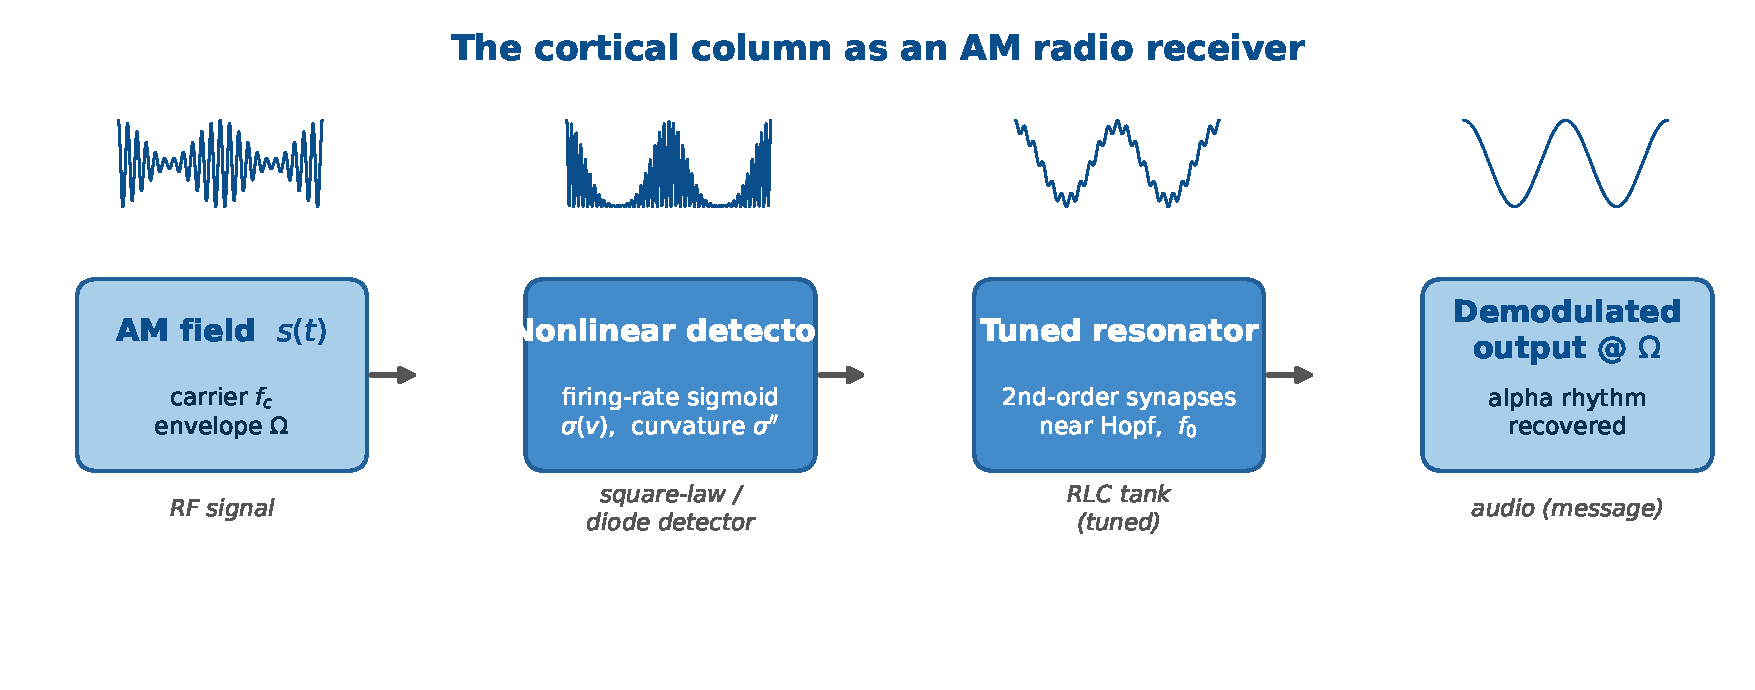
\includegraphics[width=\textwidth]{fig_concept.pdf}
%\vspace{-2cm}

\caption{\DIFdelbeginFL \DIFdelFL{\textbf{The cortical column as an AM radio receiver (schematic).} An AM field
(carrier $f_c$, envelope $\Omega$) reaches a }\DIFdelendFL \DIFaddbeginFL \DIFaddFL{\textbf{The cortical column as a tuned receiver.} A }\DIFaddendFL nonlinear detector
\DIFdelbeginFL \DIFdelFL{(}\DIFdelendFL \DIFaddbeginFL \DIFaddFL{generates }\DIFaddendFL the \DIFdelbeginFL \DIFdelFL{firing-rate
sigmoid, curvature $\Sig''$), whose output passes through }\DIFdelendFL \DIFaddbeginFL \DIFaddFL{beat at angular frequency $\Omega$ from }\DIFaddendFL a \DIFdelbeginFL \DIFdelFL{tuned resonator (the
second-order-synapse network }\DIFdelendFL \DIFaddbeginFL \DIFaddFL{carrier }\DIFaddendFL near \DIFaddbeginFL \DIFaddFL{$f_c$; }\DIFaddendFL a
\DIFdelbeginFL \DIFdelFL{Hopf, }\DIFdelendFL \DIFaddbeginFL \DIFaddFL{recurrent network amplifies it near its }\DIFaddendFL natural frequency $f_0$\DIFdelbeginFL \DIFdelFL{), recovering
a beat-frequency component as an oscillation at $\Omega$}\DIFdelendFL . The \DIFdelbeginFL \DIFdelFL{analogy is functional rather
than circuit-identical}\DIFdelendFL \DIFaddbeginFL \DIFaddFL{diagram shows
the static-sigmoid realization}\DIFaddendFL . In a \DIFdelbeginFL \DIFdelFL{classic }\DIFdelendFL \DIFaddbeginFL \DIFaddFL{conventional }\DIFaddendFL AM receiver\DIFaddbeginFL \DIFaddFL{, }\DIFaddendFL the tuned \DIFdelbeginFL \DIFdelFL{resistor--inductor--capacitor tank sits \emph{before} the detector and }\DIFdelendFL \DIFaddbeginFL \DIFaddFL{circuit
}\DIFaddendFL selects the carrier \DIFaddbeginFL \DIFaddFL{before detection }\DIFaddendFL \cite{nahin2001}; here the \DIFdelbeginFL \DIFdelFL{sigmoid generates the baseband beat component, and a
\emph{baseband} }\DIFdelendFL resonator \DIFdelbeginFL \DIFdelFL{downstream of it }\DIFdelendFL selects
\DIFdelbeginFL \DIFdelFL{and amplifies modulation frequencies
near }\DIFdelendFL the \DIFdelbeginFL \DIFdelFL{column's own rhythm, so TI ``broadcasts'' to whichever columns are tuned to its
beat frequency}\DIFdelendFL \DIFaddbeginFL \DIFaddFL{low-frequency output}\DIFaddendFL . \DIFdelbeginFL \DIFdelFL{A }\DIFdelendFL \DIFaddbeginFL \DIFaddFL{The laminar extension also has a }\DIFaddendFL carrier-selective
stage \DIFdelbeginFL \DIFdelFL{upstream of the detector does appear in the
laminar model }\DIFdelendFL (\S\ref{sec:lanmm-results}).}
\label{fig:concept}
\end{figure}

\section{Theory}

\subsection{\DIFdelbegin \DIFdel{Neural mass models }\DIFdelend \DIFaddbegin \DIFadd{Population transfer }\DIFaddend and the \DIFdelbegin \DIFdel{Jansen--Rit circuit}\DIFdelend \DIFaddbegin \DIFadd{slow-synapse limit}\DIFaddend }\label{sec:nmm}
A neural mass model \DIFdelbegin \DIFdel{(NMM) collapses the activity of a large population ($\sim 10^4$) of similar neurons into a handful of population-averaged }\DIFdelend \DIFaddbegin \DIFadd{describes a population through averaged }\DIFaddend variables
\cite{ruffini2025rosetta,jansen1995}. \DIFdelbegin \DIFdel{Two elements recur in the Jansen--Rit-type models
considered first.
First, each synapse acts as a \emph{linear filter} $\hat K$ that converts an
incoming }\DIFdelend \DIFaddbegin \DIFadd{In the Jansen--Rit (JR) family, a linear synaptic
filter converts }\DIFaddend presynaptic firing rate $r(t)$ into \DIFdelbegin \DIFdel{a postsynaptic potential (PSP)
$x(t)=\hat K[r]$; equivalently $r=\hat L[x]$ with $\hat L=\hat K^{-1}$ a
differential operator whose few coefficients set the synapse's gain, decay time }\DIFdelend \DIFaddbegin \DIFadd{postsynaptic potential $x(t)$:
}\[
\DIFadd{\ddot x+2a\dot x+a^2x=Aa\,r(t),
}\]
\DIFadd{with inverse synaptic time $a$ and gain parameter $A$; inhibitory synapses use
parameters $b$ }\DIFaddend and \DIFdelbegin \DIFdel{delay \cite{ruffini2025rosetta}. In the Jansen--Rit (JR) family the kernel is
the ``alpha function'' $h(t)=Aa\,t\,e^{-at}$ (excitatory; $B,b$ for the inhibitory synapse), i.e.\ the second-order operator
$\hat L=(Aa)^{-1}(\mathrm{d}/\mathrm{d}t+a)^2$, so each PSP obeys
$\ddot x+2a\dot x+a^2x = Aa\,r(t)$. Second, the PSPs converging on a population sum
to a mean membrane potential $v=\sum_s x_s$}\DIFdelend \DIFaddbegin \DIFadd{$B$. Summed postsynaptic potentials give the mean input $v$}\DIFaddend , which
a static \DIFdelbegin \DIFdel{, saturating
\emph{transfer function}---the sigmoid---turns back into a population }\DIFdelend \DIFaddbegin \DIFadd{transfer curve converts to }\DIFaddend firing rate \cite{wilsoncowan1972},
\DIFdelbegin \begin{displaymath}
\DIFdel{\Sig(v)=\frac{2e_0}{1+e^{\,\rho(v_0-v)}} ,
%DIFDELCMD < \label{eq:sigmoid}%%%
}\end{displaymath}%DIFAUXCMD
\DIFdelend \DIFaddbegin \begin{equation}
\DIFadd{\Sig(v)=\frac{2e_0}{1+e^{\,\rho(v_0-v)}} .
\label{eq:sigmoid}
}\end{equation}\DIFaddend
\DIFdelbegin \DIFdel{with maximal firing rate }\DIFdelend \DIFaddbegin \DIFadd{Here }\DIFaddend $2e_0$ \DIFdelbegin \DIFdel{, half-maximal at the inflection $v_0$, and slope set by
}\DIFdelend \DIFaddbegin \DIFadd{is the maximum rate, $v_0$ the inflection voltage, and }\DIFaddend $\rho$ \DIFdelbegin \DIFdel{; it saturates because firing rates are bounded \cite{ruffini2025rosetta}. The sigmoid is
the only nonlinearity in the model, and in this model it is what makes (de)modulation
possible: it is memoryless, so whatever enters its argument, a kHz carrier included, is
mapped to a rate instantaneously. That is an idealization. The curve is the ensemble
average of single-neuron input--output relations for slowly varying input, so its curvature
$\Sig''$ summarizes cellular nonlinearities (thresholds, spike generation, noise) smoothed
by the spread of states across the population. Whether a fast carrier reaches that curve
unchanged is a question the memoryless model cannot answer; the exact mean field below
(Eq.~\eqref{eq:mpr}) can, and \S\ref{sec:dynamic} shows that it does not. The network
supplies the resonant \emph{amplification} (\S\ref{sec:carrier}). Frequency-selective
resonance can also be intrinsic to single cells, through currents such as $I_h$ and $I_M$
\cite{hutcheonyarom2000}. A companion modeling manuscript by de Palma Aristides et al.\
\cite{depalma2026ti} reports cell-type- and state-dependent TI frequency selectivity in
morphologically detailed hippocampal neurons, with sensitivity to these conductances.
Such cellular tuning can coexist with recurrent amplification.
The models here isolate
the latter: second-order synapses on a loop near criticality generate resonance even
when the cells do not \cite{brunelhakim1999,brunelwang2003}.
}\DIFdelend \DIFaddbegin \DIFadd{the inverse
voltage scale. Nonzero curvature makes this curve a mixer, while its slope sets
the local gain of the recurrent circuit.
}\DIFaddend

\DIFdelbegin \DIFdel{Assembled into a network, these two elements give the }\DIFdelend \DIFaddbegin \DIFadd{For a synapse from population $n$ to $m$, the resulting }\DIFaddend NMM1 \DIFdelbegin \DIFdel{transfer-function form of
\cite{ruffini2025rosetta}
(their Eq.~6.5): for each synapse $m\!\leftarrow\!n$,
}\begin{displaymath}
\DIFdel{\hat L_{m\leftarrow n}\big[u_{m\leftarrow n}\big]=C_{m\leftarrow n}\,r_n,\qquad
v_m=\Lambda[\hat E]+\!\!\sum_{n:\,C_{m\leftarrow n}\neq0}\!\! u_{m\leftarrow n},\qquad
r_m=\Sig(v_m),
%DIFDELCMD < \label{eq:nmm1}%%%
}\end{displaymath}%DIFAUXCMD
\DIFdelend \DIFaddbegin \DIFadd{equations are
\cite{ruffini2025rosetta}
}\begin{equation}
\DIFadd{\hat L_{m\leftarrow n}\big[u_{m\leftarrow n}\big]=C_{m\leftarrow n}\,r_n,\qquad
v_m=\Lambda[\hat E]+\!\!\sum_{n:\,C_{m\leftarrow n}\neq0}\!\!u_{m\leftarrow n},\qquad
r_m=\Sig(v_m).
\label{eq:nmm1}
}\end{equation}\DIFaddend
\DIFdelbegin \DIFdel{with $u_{m\leftarrow n}$ the PSP produced at synapse $m\!\leftarrow\!n$, }\DIFdelend \DIFaddbegin \DIFadd{The operator $\hat L$ is the inverse synaptic filter, $u_{m\leftarrow n}$ its
postsynaptic potential, }\DIFaddend $C_{m\leftarrow n}$ the connectivity, and $\Lambda[\hat E]$
\DIFdelbegin \DIFdel{any \emph{direct}, non-synaptic perturbation of the membrane. An applied fieldenters precisely here, as the additive term $\Lambda[\hat E]$ in
the sigmoid's argument, }\DIFdelend \DIFaddbegin \DIFadd{the direct polarization caused by the applied field. This field contribution enters
}\DIFaddend alongside the synaptic \DIFdelbegin \DIFdel{PSPs---the starting point for
\S\ref{sec:coupling}. The concrete equations and parameters of the models simulated are
collected in App.~\ref{app:models}, in this formalism}\DIFdelend \DIFaddbegin \DIFadd{potentials, without first passing through a synapse}\DIFaddend .

\DIFdelbegin \DIFdel{This becomes exact one rung up the modeling ladder \cite{ruffini2025rosetta}. For a
network of }\DIFdelend \DIFaddbegin \DIFadd{The corresponding population nonlinearity can be derived for }\DIFaddend all-to-all coupled
\DIFdelbegin \DIFdel{quadratic integrate-and-fire (QIF ) }\DIFdelend \DIFaddbegin \DIFadd{QIF }\DIFaddend neurons with Lorentzian-distributed excitabilities\DIFdelbegin \DIFdel{, the Ott--Antonsen ansatz yields a
\emph{closed, exact} mean field for the population }\DIFdelend \DIFaddbegin \DIFadd{. Their exact
Montbri\'o--Paz\'o--Roxin (MPR) mean field evolves the }\DIFaddend firing rate $r$ and mean \DIFdelbegin \DIFdel{potential }\DIFdelend \DIFaddbegin \DIFadd{voltage
}\DIFaddend $v$ \DIFdelbegin \DIFdel{---the next-generation (Montbri\'o--Paz\'o--Roxin, MPR) mass
\cite{montbrio2015}, completed with the second-order synapses of neural-mass models
in the exact ``}\DIFdelend \DIFaddbegin \DIFadd{\cite{montbrio2015}; adding dynamic synapses gives }\DIFaddend NMM2
\DIFdelbegin \DIFdel{'' theory \cite{ruffini2021nmm2,clusella2023}:
}\begin{displaymath}
\DIFdel{\dot r=\frac{\Delta}{\pi}+2rv,\qquad
\dot v=v^2+\bar\eta-\pi^2 r^2+I(t),
%DIFDELCMD < \label{eq:mpr}%%%
}\end{displaymath}%DIFAUXCMD
\DIFdelend \DIFaddbegin \DIFadd{\cite{ruffini2021nmm2,clusella2023}. In membrane-time units,
}\begin{equation}
\DIFadd{\dot r=\frac{\Delta}{\pi}+2rv,\qquad
\dot v=v^2+\bar\eta-\pi^2r^2+I(t),
\label{eq:mpr}
}\end{equation}\DIFaddend
\DIFdelbegin \DIFdel{with the applied current $I(t)$ entering linearly,
the common background excitability
}\DIFdelend \DIFaddbegin \DIFadd{where }\DIFaddend $\bar\eta$ \DIFdelbegin \DIFdel{(the bifurcation parameter), and the heterogeneity }\DIFdelend \DIFaddbegin \DIFadd{is the mean excitability, $\Delta>0$ its }\DIFaddend half-width\DIFdelbegin \DIFdel{$\Delta$ setting the smoothing. Here the nonlinearity is \emph{derived, not postulated}: the quadratic $v^2$ term, inherited from the
single-neuron QIF dynamics, mixes whatever the membrane potential
carries, and the applied current enters the voltage equation rather than a rate map}\DIFdelend \DIFaddbegin \DIFadd{, and $I(t)$ the
normalized input, including recurrent drive when present. Rate and voltage are
expressed in the corresponding rescaled units}\DIFaddend . For a constant \DIFdelbegin \DIFdel{input $Q$ the population settles on the rate $r=F(Q)$, }\begin{displaymath}
\DIFdel{F(Q)=\frac{1}{\pi}\sqrt{\frac{Q+\sqrt{Q^2+\Delta^2}}{2}},
%DIFDELCMD < \label{eq:Fmpr}%%%
}\end{displaymath}%DIFAUXCMD
\DIFdelend \DIFaddbegin \DIFadd{total drive
$Q=\bar\eta+I$, setting both derivatives to zero gives $v=-\Delta/(2\pi r)$ and
}\begin{equation}
\DIFadd{r=F(Q)=\frac{1}{\pi}\sqrt{\frac{Q+\sqrt{Q^2+\Delta^2}}{2}} .
\label{eq:Fmpr}
}\end{equation}\DIFaddend
\DIFdelbegin \DIFdel{a sigmoid-like curve with a convex foot, }\DIFdelend \DIFaddbegin \DIFadd{This nonlinear curve exists without recurrent coupling. It has }\DIFaddend an inflection at
$Q=\Delta/\sqrt3$ and an unbounded concave rise\DIFdelbegin \DIFdel{\cite{clusella2023}; it is the slow-input limit of the dynamics,
not a logistic. The Jansen--Rit sigmoid is the heuristic (NMM1) stand-in for such a curve. Both
models mix two carriers quadratically, but their detector coefficients are not the same
object: the memoryless sigmoid's is its curvature, the MPR population's depends on the carrier frequency through the voltage dynamics (\S\ref{sec:dynamic}). The same exact
theory exhibits weak-field resonance and Arnold tongues that sharpen with self-coupling
\cite{clusella2023,ruffini2021nmm2}, the near-Hopf amplification we exploit below. }\DIFdelend \DIFaddbegin \DIFadd{, unlike the saturating JR sigmoid.
}\DIFaddend

\DIFdelbegin \DIFdel{\emph{What the transfer functions represent.} In every model the demodulating object is }\DIFdelend \DIFaddbegin \DIFadd{If the population relaxes to this equilibrium faster than synaptic inputs change,
NMM2 reduces to a static rate map with dynamic synapses
\cite{ruffini2021nmm2,clusella2023}. Restoring the membrane time $\tau_m$ and physical
firing rate, }\DIFaddend a \DIFdelbegin \DIFdel{\emph{population} input--output map rather than a passive somatic membrane element. In JR/LaNMM it
is the sigmoid \eqref{eq:sigmoid}, the
effective transfer of an excitable neuronal ensemble
(mean PSP in, population firing rate out); in NMM2 the same role is played by the exact MPR
quadratic \eqref{eq:mpr}. Its curvature is the mesoscopic trace of cellular nonlinearities
(thresholds, spike generation, refractoriness, noise, saturation), so for inputs slow compared with the population's own dynamics, reading the demodulation
off $\Sig''$ is legitimate at this scale; for a fast carrierthe derived $v^2$ term mixes
the voltage excursion and the population curve enters as the read-out gain
(\S\ref{sec:dynamic}).
The membrane low-pass does not contradict this: it bears on \emph{access}---how the carrier
reaches the nonlinearity---not on legitimacy.Because an applied field polarizes the membrane
directly, in parallel, at every compartment (\S\ref{sec:coupling}), access is set by the entry point, and }\DIFdelend \DIFaddbegin \DIFadd{second-order synapse with time constant $\tau_s$ obeys
}\begin{equation}
\DIFadd{r(t)\simeq \frac{F(Q(t))}{\tau_m},\qquad
\tau_s^2\ddot s_{\rm syn}+2\tau_s\dot s_{\rm syn}+s_{\rm syn}=r(t),
\label{eq:slow_synapse}
}\end{equation}
\DIFadd{where $s_{\rm syn}$ is }\DIFaddend the \DIFdelbegin \DIFdel{open biophysical question is which fast compartment (axon initial
segment, node, or channel) still passes a kHz carrier to that nonlinear transfer
(\S\ref{sec:khz}).
Once the carrier is sampled there,
}\DIFdelend \DIFaddbegin \DIFadd{filtered rate entering the recurrent drive in $Q$, with the original
coupling normalization retained. This is }\DIFaddend the \DIFdelbegin \DIFdel{neural mass describes the
population-level demodulation and near-Hopf amplification of the recovered beat component}\DIFdelend \DIFaddbegin \DIFadd{slow-synapse limit: shortening the
effective membrane time makes the transfer appear static while the network retains
its synaptic dynamics. The relevant separation is between the population relaxation
time $\tau_{\rm rel}$ and $\tau_s$. Applying the same static map directly to a
carrier of angular frequency $\omega_c$ requires the stronger condition
$\omega_c\tau_{\rm rel}\ll1$. A population can therefore be quasistatic for its
synaptic inputs yet dynamic for a kHz carrier}\DIFaddend .

\DIFaddbegin \DIFadd{The transfer curve summarizes cellular nonlinearities only within this regime.
The exact QIF reduction includes its spike-generating quadratic and excitability
distribution; it does not by itself reproduce the sodium-channel kinetics implicated
by Luff et al.\ \cite{luff2024mixer}. Those mechanisms can enter an effective
population description through a calibrated dynamic input--output functional.
A steady-state rate curve alone does not specify its frequency dependence.
Section~\ref{sec:dynamic} calculates this dependence for QIF and recovers
Eq.~\eqref{eq:Fmpr} in the adiabatic limit.
}

\DIFadd{Cellular and circuit resonance are also distinct. Conductances such as $I_h$ and
$I_M$ can tune single neurons \cite{hutcheonyarom2000}; the companion manuscript of
de Palma Aristides et al.\ \cite{depalma2026ti} reports cell-type- and state-dependent
TI frequency selectivity in hippocampal neurons, sensitive to these conductances.
Recurrent excitatory--inhibitory circuits can generate resonance without intrinsic
cellular resonance \cite{brunelhakim1999,brunelwang2003}. In the fast-membrane limit,
any retained resonance belongs to the remaining synaptic circuit; modes requiring
finite membrane dynamics need not persist.
}

\DIFaddend The \DIFdelbegin \DIFdel{single }\DIFdelend JR column couples \DIFdelbegin \DIFdel{a pyramidalpopulation to one excitatory and one inhibitory
interneuron population through this synapse$+$sigmoid motif, with the field entering }\DIFdelend \DIFaddbegin \DIFadd{pyramidal, excitatory-interneuron, and inhibitory-interneuron
populations, with field input to }\DIFaddend the pyramidal sigmoid \DIFdelbegin \DIFdel{as $s(t)=\Lambda[\hat E]$ (\S\ref{sec:coupling}) and the }\DIFdelend \DIFaddbegin \DIFadd{and }\DIFaddend local field potential
(LFP) proxy $v=y_1-y_2$ \DIFdelbegin \DIFdel{. Its equations (Eqs.~\eqref{eq:jr0}) and parameters (Table~\ref{tab:params}) are
collected in }\DIFdelend \DIFaddbegin \DIFadd{(}\DIFaddend App.~\ref{app:models}\DIFdelbegin \DIFdel{.
}%DIFDELCMD <

%DIFDELCMD < %%%
\DIFdel{For the biophysical realization (\S\ref{sec:lanmm-results})we use a second model
built from the same ingredients: the laminar neural mass model }\DIFdelend \DIFaddbegin \DIFadd{). The laminar extension }\DIFaddend (LaNMM)
\cite{ruffini2025cfc,sanchezTodo2023} \DIFdelbegin \DIFdel{, which embeds this synapse$+$sigmoid motif in
a two-band cortical column---a deep
Jansen--Rit-like subcircuit (}\DIFdelend \DIFaddbegin \DIFadd{adds coupled alpha and gamma circuits: deep
}\DIFaddend pyramidal $P_1$\DIFdelbegin \DIFdel{with }\DIFdelend \DIFaddbegin \DIFadd{, }\DIFaddend spiny-stellate (SS)\DIFaddbegin \DIFadd{, }\DIFaddend and somatostatin (SST) \DIFdelbegin \DIFdel{interneurons; intrinsic alpha, $\sim$10~Hz) coupled to a
superficial PING-like (pyramidal--interneuron network
gamma) subcircuit (}\DIFdelend \DIFaddbegin \DIFadd{populations, and a
superficial }\DIFaddend pyramidal $P_2$\DIFdelbegin \DIFdel{with PV interneurons; intrinsic gamma,
$\sim$40~Hz). The single JR column lets us isolate and
analyze the
mechanism; the LaNMM then exhibits it in a column with its own fast/slow loops and two native resonances. Everything below applies to both: the field enters the sigmoid argument as a
membrane polarization, and the recovered beat component drives a resonant circuit}\DIFdelend \DIFaddbegin \DIFadd{/PV circuit. These models retain dynamic synapses and
static rate curves; NMM2 and its spiking realization retain membrane dynamics as well}\DIFaddend .

\subsection{From applied field to a squared-envelope beat component}\label{sec:coupling}
We \DIFdelbegin \DIFdel{model the applied TI }\DIFdelend \DIFaddbegin \DIFadd{use the quasistatic electromagnetic approximation for the applied }\DIFaddend field $E(t)$
(V/m)\DIFdelbegin \DIFdel{as a quasi-static perturbation of the
membrane potential that the spike-generating nonlinearity reads. ``Quasi-static''
means we neglect electromagnetic }\DIFdelend \DIFaddbegin \DIFadd{, neglecting }\DIFaddend propagation and induction\DIFdelbegin \DIFdel{(wavelengths $\gg$
head, frequencies far below tissue relaxation), so the field acts as an
instantaneouspolarization added inside the firing-rate map,
}\DIFdelend \DIFaddbegin \DIFadd{. This does not make membrane charging
instantaneous. Let $s(t)$ be the polarization after the cellular access response;
the static population model reads
}\DIFaddend \begin{equation}
r(t)=\Sig\!\big(v(t)+s(t)\big),\qquad
E(t)=E_1\cos\omega_1 t+E_2\cos\omega_2 t .
\label{eq:coupling}
\end{equation}
\DIFdelbegin \DIFdel{Unlike synaptic drive, an applied field does not enter through the synaptic kernel:
it polarizes the membrane directly and simultaneously at every compartment---soma, dendrite}\DIFdelend \DIFaddbegin \DIFadd{The field acts directly on soma, dendrites}\DIFaddend , axon initial segment (AIS), \DIFdelbegin \DIFdel{terminal---each }\DIFdelend \DIFaddbegin \DIFadd{and terminals,
each }\DIFaddend with its own coupling and \DIFdelbegin \DIFdel{its
own access filter. The perturbation $s(t)$ reaching the nonlinearity is therefore a sum over these }\DIFdelend \DIFaddbegin \DIFadd{frequency response. In a reduced description, their
contributions to the effective input are represented by }\DIFaddend parallel entry points,
\DIFdelbegin \DIFdel{or ``doors'',
}\DIFdelend \begin{equation}
s(t)=\sum_c \boldsymbol\lambda^c_f\!\cdot\!\mathbf E(t),\qquad
\lambda^c_f=\lambda^c_0\,\lvert H_c(\omega_c)\rvert,
\label{eq:doors}
\end{equation}
where $\lambda^c_0$ is the \DIFdelbegin \DIFdel{DC (quasi-static) coupling of door }\DIFdelend \DIFaddbegin \DIFadd{static polarization length of compartment }\DIFaddend $c$\DIFdelbegin \DIFdel{---the weak-field
polarization length $\delta V=\boldsymbol\lambda\!\cdot\!\mathbf E$ of transcranial-stimulation modeling \cite{ruffini2025rosetta,galangadea2023}---and $\lambda^c_f$ is its effective coupling at the carrier, the DC value rolled off by that door's own filter
$H_c$. Both are limits of one compartment equation }\DIFdelend ,
\DIFdelbegin \DIFdel{$C\dot{\mathbf V}+A\mathbf V=\mathbf I^0-\mathbf p\,E$
\cite{ruffini2021nmm2} , whose response to an alternating field is
$\delta\mathbf V(\omega)=-(A+i\omega C)^{-1}\mathbf p\,E(\omega)$: the quasi-static $\lambda_0$ is
its value at $\omega\to0$ and $H_c$ }\DIFdelend \DIFaddbegin \DIFadd{$H_c$ its access filter, and $\omega_c=2\pi f_c$
\cite{ruffini2025rosetta,galangadea2023}. Equation~\eqref{eq:doors} uses amplitude
gains; relative phases can be retained in the complex transfer. The passive
compartment equation $C\dot{\mathbf V}+A\mathbf V=\mathbf I^0-\mathbf pE$
\cite{ruffini2021nmm2} gives
$\delta\mathbf V(\omega)=-(A+i\omega C)^{-1}\mathbf pE(\omega)$, with capacitance
matrix $C$, conductance matrix $A$, endogenous current $\mathbf I^0$, and field-to-current
coupling $\mathbf p$. The static gain and }\DIFaddend its frequency dependence \DIFaddbegin \DIFadd{belong to this
one response. A model driven by post-coupling polarization and a model driven by
current through its own membrane equation must therefore count that filtering once}\DIFaddend .
\DIFdelbegin \DIFdel{Prescribing $\lambda_0E$ inside a
static sigmoid and injecting the current $\mathbf p\,E$ into a model that carries its own $C\dot V$, as the exact mean field does (\S\ref{sec:dynamic}), are the two ends of this one
chain; the membrane filter is applied onceeither way, and a comparison of the two detectors
is only meaningful with the field inserted at the same point.
The field is thus not only a somatic membrane perturbation, and which door
dominates is set by the
carrier: at DC the soma/dendrite has the largest coupling (the
whole-cell dipole), but its filter cuts it at kHz while a fast door stays open, so
$\lambda^{\rm soma}_f$ collapses and the dominant term crosses over (\S\ref{sec:khz}).
The amplitudes }\DIFdelend \DIFaddbegin

\DIFadd{For a dominant entry point, $\varepsilon_j=\lambda_f(\omega_j)E_j$ denotes the
polarization }\DIFaddend reaching the nonlinearity\DIFdelbegin \DIFdel{are the post-coupling polarizations
$\varepsilon_j=\lambda_f E_j$ of the open door (door index suppressed when only the open
door matters), which is what Eq. ~\eqref{eq:am} contains rather than the raw applied field. The main text takes
the favorable direct limit in
which a fast door (axonal or nodal) samples the carrier before appreciable
attenuation, $\lambda_f\!\approx\!\lambda_0$, isolating the sigmoid$+$resonance
principle}\DIFdelend \DIFaddbegin \DIFadd{. The direct-coupling calculation takes
$\lambda_f\approx\lambda_0$ to isolate mixing and recurrent amplification}\DIFaddend ;
\S\ref{sec:khz} restores \DIFdelbegin \DIFdel{the roll-off and shows the carrier dependence
entering quadratically, $A_\Omega\propto\lvert H_c(f_c)\rvert^2$}\DIFdelend \DIFaddbegin \DIFadd{frequency-dependent access. A fast compartment could
justify this approximation, but its identity and coupling are not inferred from
the population model}\DIFaddend .

Expanding $\Sig$ about an operating point $v^*$ (a Volterra/Taylor expansion, as
in \cite{ruffini2025ham}) gives
$\Sig(v^*+s)\approx\Sig(v^*)+\Sig'(v^*)\,s+\half\Sig''(v^*)\,s^2+\dots$
The truncation \DIFdelbegin \DIFdel{holds only while $|s|$ is small against the sigmoid's voltage scale
$1/\rho\approx1.8$~mV . Human TI polarizations are $\sim 10^{-2}$~mV, over two orders below
that, so the quadratic term is the leadingnonlinearity throughout the regime this paper
treats. Rodent TI is not in that regime: the fields are $\sim 10^3$ times larger, the
sigmoid saturates, and the expansion fails.
\S\ref{sec:discussion} returns to what that
costs when rodent results are scaled to humans.
Intuitively, the difficulty is that the field carries power only near the carrier
$\omega_c$, far from the slow envelope frequency $\Omega$, so some operation must move
power down to $\Omega$. The \emph{linear} term cannot: it passes the input lines straight
through, reproducing the carrier and its two flanking \emph{sidebands} (the lines at
$\omega_c\pm\Omega$ created by the modulation), but still nothing at $\Omega$. The \emph{quadratic} term
can: squaring the field multiplies the fast carrier by itself, and
because $\cos^2$ has a constant (zero-frequency) part, the squaring folds power down to
\emph{baseband}---the low-frequency band near $0$~Hz, where the slow envelope lives. This
is \emph{rectification}, what a diode does in an AM radio. The }\DIFdelend \DIFaddbegin \DIFadd{requires $|s|\ll1/\rho\approx1.8$~mV and a nonzero second derivative
for quadratic mixing to be leading. Larger excursions require the full transfer curve.
The linear term preserves the two input frequencies. The quadratic cross term
generates their difference through the }\DIFaddend identity
$2\cos\omega_1t\cos\omega_2t=\cos\Omega t+\cos(\omega_1+\omega_2)t$\DIFdelbegin \DIFdel{shows where the beat
comes from: the cross term of $s^2$}\DIFdelend .
Averaging over the carrier (the fast
$\cos^2\omega_jt$ terms average to $\half$, the sum-frequency term to zero),
\begin{equation}
\big\langle\Sig(v^*+s)\big\rangle_c
=\Sig(v^*)+\tfrac14\Sig''(v^*)\,(\varepsilon_1^2+\varepsilon_2^2)
+\tfrac12\Sig''(v^*)\,\varepsilon_1\varepsilon_2\cos\Omega t+O(\varepsilon^4),
\label{eq:taylor}
\end{equation}
so a line appears at exactly the envelope frequency $\Omega$, with amplitude
\begin{equation}
A_\Omega\simeq\half\,\Sig''(v^*)\,\varepsilon_1\varepsilon_2 ,
\label{eq:demod}
\end{equation}
where $\simeq$ means to leading order in the polarizations, here and in what follows. The
same expansion leaves a constant (DC) term, $\tfrac14\Sig''(\varepsilon_1^2+\varepsilon_2^2)$,
which any read-out of the mean rate must include.

What the quadratic term recovers is not the envelope but its square. Writing $A(t)$ for
the instantaneous envelope of the two-tone field,
$A^2(t)=\varepsilon_1^2+\varepsilon_2^2+2\varepsilon_1\varepsilon_2\cos\Omega t$, the
low-pass part of the squared signal is exactly
\begin{equation}
\mathrm{LPF}\big[s^2(t)\big]=\half A^2(t)
=\frac{\varepsilon_1^2+\varepsilon_2^2}{2}+\varepsilon_1\varepsilon_2\cos\Omega t .
\label{eq:sqenv}
\end{equation}
This is square-law detection in the strict sense: the population transduces $A^2$, not
$A$. The distinction matters because $A^2$ is exactly sinusoidal at $\Omega$
whereas $A$ is not---at a matched target ($\varepsilon_1=\varepsilon_2=\varepsilon$),
$A(t)=2\varepsilon|\cos(\Omega t/2)|$, a rectified cosine.

\emph{The amplitude-modulated surrogate.} The dense perturbative sweeps below use the
three-line waveform
\begin{equation}
s(t)=\varepsilon\,[\,1+m\cos\Omega t\,]\cos\omega_c t,\qquad \omega_c=2\pi f_c ,
\label{eq:amsur}
\end{equation}
with modulation depth $m$, because it parameterizes a sweep by one amplitude. It is not
the physical signal: it carries a line at $\omega_c$ that the two-tone sum lacks. The two
agree at $\Omega$ to leading order (the surrogate gives
$A_\Omega=\half\Sig''\varepsilon^2m$) and are \emph{not} equivalent beyond it. For matched genuine tones $\mathrm{LPF}[s^2]=\varepsilon^2(1+\cos\Omega t)$,
whereas for the $m=1$ AM surrogate
$\mathrm{LPF}[s^2]=\varepsilon^2(\tfrac34+\cos\Omega t+\tfrac14\cos2\Omega t)$: the same
$\Omega$ amplitude, but a different DC term and a spurious second harmonic at $25\%$ of
the fundamental. Since that second harmonic is precisely the observable that
distinguishes transduction classes (\S\ref{sec:transduction}), every claim that turns on
the waveform is run with genuine two tones: the demodulation demonstration
(Fig.~\ref{fig:demod}), the curvature and square-law controls (Fig.~\ref{fig:opp}), the
laminar maps (Figs.~\ref{fig:lanmm_p2},~\ref{fig:lanmm_p1}) and the kHz demonstration.
The AM surrogate is retained for the dense perturbative sweeps in $(\Omega,p)$ and
$(\Omega,C)$, which read only the leading $\Omega$ component, and
Fig.~\ref{fig:opp}d verifies that the two agree there.

In the language of \cite{ruffini2025ham}, the quadratic cross-term $s_1 s_2$ between a
slow and a fast input (the second-order Volterra kernel) implements amplitude
modulation/demodulation and the associated intermodulation lines.
Demodulation is thus itself an intermodulation product: the line at $\Omega$ is the
\emph{difference frequency} of the two applied tones ($\omega_1$ and $\omega_2$),
generated by the same quadratic term \DIFdelbegin \DIFdel{that---acting a second time, now }\DIFdelend \DIFaddbegin \DIFadd{that, acting again }\DIFaddend on an intrinsic
rhythm $\omega_0$\DIFdelbegin \DIFdel{---produces }\DIFdelend \DIFaddbegin \DIFadd{, produces }\DIFaddend the $\omega_0\pm\Omega$ sidebands seen at the spiking level
(Fig.~\ref{fig:qif_timing}b).
\DIFdelbegin \DIFdel{One nonlinear mixer, applied in cascade.
}\DIFdelend Equation~\eqref{eq:demod} carries three predictions, all verified below: the
recovered amplitude is quadratic in the drive ($A_\Omega\propto\varepsilon^2$,
square-law detection); it follows the sigmoid curvature
($A_\Omega\propto\Sig''(v^*)$, hence zero at the inflection $v^*=v_0$); and, \emph{at
fixed post-coupling polarization} $\varepsilon$, it is independent of the carrier
$\omega_c$. This last prediction needs care: as a function of the \emph{applied} field the
response inherits the coupling $\varepsilon=\lambda_f E_0$, so the field required for a
given effect rises with $f_c$ (\S\ref{sec:khz})---consistent with the experimental
consensus. Carrier independence is thus a statement about the recovered beat component at fixed
polarization, not about the applied field.

\subsection{\DIFdelbegin \DIFdel{Static transfer versus dynamic mixing: the }\DIFdelend \DIFaddbegin \DIFadd{The }\DIFaddend exact mean field \DIFaddbegin \DIFadd{connects static and dynamic mixing}\DIFaddend }\label{sec:dynamic}
The \DIFdelbegin \DIFdel{sigmoid of Eq.~\eqref{eq:demod} is memoryless, so the carrier traverses the curve and
the curvature is the detector at any carrier frequency. A population of neurons is not
memoryless: its rate relaxes and rings on its own timescales, and an applied current
polarizes the membrane before any spike-generating nonlinearity sees it. The exact mean
field makes the consequence explicit. Take a single }\DIFdelend \DIFaddbegin \DIFadd{adiabatic condition in \S\ref{sec:nmm} determines whether the static curve describes
carrier mixing. Consider an uncoupled }\DIFaddend MPR population (Eq.~\eqref{eq:mpr}, \DIFdelbegin \DIFdel{$\tau=1$, no coupling)with constant input }\DIFdelend \DIFaddbegin \DIFadd{membrane
time set to one), with constant drive }\DIFaddend $Q$ and a weak \DIFdelbegin \DIFdel{current carrier }\DIFdelend \DIFaddbegin \DIFadd{added current }\DIFaddend $a\cos\omega t$\DIFdelbegin \DIFdel{added to the voltage equation.
Expanding to }\DIFdelend \DIFaddbegin \DIFadd{.
To }\DIFaddend second order in $a$\DIFdelbegin \DIFdel{and averaging over the
carrier, the rate acquires a constant shift $a^2\,C(Q,\omega)$ with
}\begin{displaymath}
\DIFdel{C(Q,\omega)=\frac{r^*\,[\omega^2+3d^2-\nu^2]}{(d^2+\nu^2)\{[d^2+\nu^2-\omega^2]^2+4d^2\omega^2\}},
\qquad r^*=F(Q),\quad d=\frac{\Delta}{\pi r^*},\quad \nu=2\pi r^*,
%DIFDELCMD < \label{eq:crossover}%%%
}\end{displaymath}%DIFAUXCMD
\DIFdel{where
}\DIFdelend \DIFaddbegin \DIFadd{, the carrier-averaged rate shift is $a^2C(Q,\omega)$, where
}\begin{equation}
\DIFadd{C(Q,\omega)=\frac{r^*\,[\omega^2+3d^2-\nu^2]}{(d^2+\nu^2)\{[d^2+\nu^2-\omega^2]^2+4d^2\omega^2\}},
\qquad r^*=F(Q),\quad d=\frac{\Delta}{\pi r^*},\quad \nu=2\pi r^*.
\label{eq:crossover}
}\end{equation}
\DIFadd{The fixed-point eigenvalues are $-d\pm i\nu$: }\DIFaddend $d$ is the \DIFdelbegin \DIFdel{population's }\DIFdelend relaxation rate and $\nu$
\DIFdelbegin \DIFdel{its ringing frequency (the
linearization about the fixed point has eigenvalues $-d\pm i\nu$). Its two limits are
the
two detectors,
}\begin{displaymath}
\DIFdel{C(Q,\omega)\xrightarrow[\ \omega\to0\ ]{}\tfrac14F''(Q),\qquad
C(Q,\omega)\xrightarrow[\ \omega\gg\nu\ ]{}\frac{F'(Q)}{2\omega^2}.
\label{eq:crossover_limits}
}\end{displaymath}%DIFAUXCMD
\DIFdelend \DIFaddbegin \DIFadd{the ringing angular frequency, both in membrane-time units. The limiting responses are
}\begin{equation}
\DIFadd{C(Q,\omega)\xrightarrow[\ \omega\to0\ ]{}\tfrac14F''(Q),\qquad
C(Q,\omega)\xrightarrow[\ \omega\gg d,\nu\ ]{}\frac{F'(Q)}{2\omega^2}.
\label{eq:crossover_limits}
}\end{equation}\DIFaddend
\DIFdelbegin \DIFdel{For a slow carrier the }\DIFdelend \DIFaddbegin \DIFadd{In the first limit the }\DIFaddend population tracks its \DIFdelbegin \DIFdel{steady-state curve and the static curvature
rectifies, as in the Jansen--Rit calculation. For a fast carrier the voltage responds as an
integrator, with an excursion $\sim a/\omega$ and a quarter-cycle lag; the $v^2$ term mixes
that excursion into a constant, and the population converts the constant to a rate through its \emph{slope}. The coefficient is then positive whatever the operating point and largest
at the inflection, where $F''$ vanishes. }\DIFdelend \DIFaddbegin \DIFadd{static curve, whose curvature rectifies
the input. In the second, the voltage excursion is approximately $a/\omega$; its
square supplies a slow drive that the population reads through $F'$. }\DIFaddend Above the
inflection \DIFdelbegin \DIFdel{the two }\DIFdelend \DIFaddbegin \DIFadd{of $F$, these }\DIFaddend limits have opposite signs and the coefficient \DIFdelbegin \DIFdel{changes sign }\DIFdelend \DIFaddbegin \DIFadd{vanishes }\DIFaddend at
$\omega_z=\sqrt{\nu^2-3d^2}$ (Fig.~\ref{fig:crossover}a). The \DIFdelbegin \DIFdel{crossover sits at the population's own frequency, tens of
hertz for the gamma-generating PING of \S\ref{sec:nmm2-results}; the }\DIFdelend $300$~Hz \DIFdelbegin \DIFdel{carrier used
there, and TI's kHz carriers
, }\DIFdelend \DIFaddbegin \DIFadd{and kHz carriers
}\DIFaddend are on the fast side \DIFdelbegin \DIFdel{.
}\DIFdelend \DIFaddbegin \DIFadd{for the PING parameters used below. That classification is
parameter-dependent: a shorter effective membrane time can bring the same physical
carrier into the adiabatic regime.
}\DIFaddend

\DIFdelbegin \DIFdel{The two limits are not two carrier penalties.
The linear response of the voltage to the
current }\DIFdelend \DIFaddbegin \DIFadd{Membrane access is already included in this calculation. The linear voltage response
}\DIFaddend is $H_v(\omega)=(i\omega+d)/[(i\omega+d)^2+\nu^2]$\DIFdelbegin \DIFdel{, the population's own membrane:
state-shaped below $\nu$, the bare capacitance $1/(i\omega)$ above it. Dividing $C$ by $|H_v|^2$ gives the detector }\DIFdelend \DIFaddbegin \DIFadd{. Dividing by its squared magnitude
gives the mixing }\DIFaddend coefficient at fixed voltage excursion,
\DIFdelbegin \begin{displaymath}
\DIFdel{K(\omega)=\frac{C(Q,\omega)}{|H_v(\omega)|^2}
=\frac{F'(Q)}{2}\;\frac{\omega^2+3d^2-\nu^2}{\omega^2+d^2},
%DIFDELCMD < \label{eq:kfixed}%%%
}\end{displaymath}%DIFAUXCMD
\DIFdelend \DIFaddbegin \begin{equation}
\DIFadd{K(\omega)=\frac{C(Q,\omega)}{|H_v(\omega)|^2}
=\frac{F'(Q)}{2}\;\frac{\omega^2+3d^2-\nu^2}{\omega^2+d^2}.
\label{eq:kfixed}
}\end{equation}\DIFaddend
\DIFdelbegin \DIFdel{which is bounded: it runs from the static curvature per unit squared excursion at
$\omega\to0$ }\DIFdelend \DIFaddbegin \DIFadd{This coefficient tends }\DIFaddend to $F'/2$ \DIFdelbegin \DIFdel{for $\omega\gg\nu$, vanishes at $\omega_z$, and carries no power of
$\omega$ above the population's rates. All of the }\DIFdelend \DIFaddbegin \DIFadd{at high frequency. The }\DIFaddend $1/\omega^2$ \DIFaddbegin \DIFadd{suppression
}\DIFaddend at fixed current \DIFdelbegin \DIFdel{sits in
}\DIFdelend \DIFaddbegin \DIFadd{comes from }\DIFaddend $|H_v|^2$\DIFdelbegin \DIFdel{: it is the membrane term $\tau\dot v$ integrating the injected current, the same
low-pass that }\DIFdelend \DIFaddbegin \DIFadd{, the membrane filtering already represented
by }\DIFaddend Eq.~\eqref{eq:doors}\DIFdelbegin \DIFdel{places in front of the sigmoid, here computed by the model
rather than assumed. Since $F''=4r^*(3d^2-\nu^2)/(d^2+\nu^2)^3$, the inflection of $F$ is the
point $\nu^2=3d^2$, and above it the fast coefficient $F'/2$ and the static curvature have
opposite signs. Relative to a static curve
read on }\DIFdelend \DIFaddbegin \DIFadd{; it is not an additional detector filter. A static curve
placed after }\DIFaddend the same membrane \DIFdelbegin \DIFdel{, the dynamics therefore
multiply the fast-carrier coefficient by $d^2/(3d^2-\nu^2)$, a constant set by the operating
point ($0.35$, $0.66$ and $-0.03$ at $r^*\approx10$, $17$ and $37$~Hz for $\tau=15$~ms,
$\Delta=1$), not a further roll-off. With matched access the memoryless and the dynamic
detector share the leading carrier scaling; the detector sets the prefactor, its sign and its structure near the population's own frequencies}\DIFdelend \DIFaddbegin \DIFadd{has the same leading carrier roll-off, although
its mixing coefficient and sign can differ. The steady-state curvature is
$F''=4r^*(3d^2-\nu^2)/(d^2+\nu^2)^3$, so the inflection occurs at $\nu^2=3d^2$}\DIFaddend .

\DIFdelbegin \DIFdel{The same reasoning fixes what a two-tone field generates in }\DIFdelend \DIFaddbegin \DIFadd{For }\DIFaddend the full eight-state PING \DIFdelbegin \DIFdel{of
}\DIFdelend \DIFaddbegin \DIFadd{(}\DIFaddend Eq.~\eqref{eq:nmm2-ping}\DIFdelbegin \DIFdel{. In the fast-carrier limit each tone's voltage phasor is
}\DIFdelend \DIFaddbegin \DIFadd{), each high-frequency current
tone of amplitude $a_j$ produces a voltage phasor }\DIFaddend $a_j/(i\omega_j\tau_E)$\DIFdelbegin \DIFdel{, and the }\DIFdelend \DIFaddbegin \DIFadd{.
The }\DIFaddend $v_E^2$ term \DIFdelbegin \DIFdel{produces }\DIFdelend \DIFaddbegin \DIFadd{therefore supplies }\DIFaddend a difference-frequency source of magnitude
$a_1a_2/(\tau_E^2\omega_1\omega_2)$ \DIFdelbegin \DIFdel{in the $\tau_E$-divided voltage equation ,
independent of the operating point; the response is that source passed }\DIFdelend \DIFaddbegin \DIFadd{inside the equation for $\tau_E\dot v_E$.
After division by $\tau_E$, this source is propagated }\DIFaddend through the network
\DIFdelbegin \DIFdel{'s }\DIFdelend susceptibility at $\Omega$. \DIFdelbegin \DIFdel{Against the exact second-order response (full
quadratic source and full resolvent) at }\DIFdelend \DIFaddbegin \DIFadd{At }\DIFaddend four stable operating points, the \DIFdelbegin \DIFdel{fast-carrier
source is }\DIFdelend \DIFaddbegin \DIFadd{resulting
response agrees with the full second-order calculation to }\DIFaddend within $1.1\%$ at
$300$~Hz, $0.1\%$ at $1$~kHz\DIFaddbegin \DIFadd{, }\DIFaddend and $0.03\%$ at $2$~kHz
(Fig.~\ref{fig:crossover}b).
\DIFdelbegin \DIFdel{Two consequences carry through the paper. Agreement in the
$\varepsilon^2$ scaling between the sigmoid and }\DIFdelend \DIFaddbegin

\DIFadd{The carrier and beat have different routes to the firing rate. At high frequency,
}\DIFaddend the \DIFdelbegin \DIFdel{exact mean field does not mean the same
detector: the coefficients and their operating-point dependence differ, and the sign
reversal of Eq. ~\eqref{eq:demod} at the inflection is a property of the memoryless model.
And carrier independence at fixed polarization survives in the dynamic model,
with
polarization now the carrier-frequency voltage excursion $a_j/(\omega_j\tau_E)$: at fixed
current the generated source rolls off as $1/(\omega_1\omega_2)$ from the membrane dynamics
themselves. The rate's own linear response falls faster, as $1/\omega^2$: the membrane
integrates the drive into the voltage }\DIFdelend \DIFaddbegin \DIFadd{voltage equation integrates the input once, }\DIFaddend and the rate equation integrates
the voltage again, \DIFdelbegin \DIFdel{which is
what a dynamic transfer function shows when it is driven at the carrier}\DIFdelend \DIFaddbegin \DIFadd{giving a linear rate response proportional to $1/\omega^2$}\DIFaddend .
The beat \DIFdelbegin \DIFdel{does not
inherit the second power, because the product is formed }\DIFdelend \DIFaddbegin \DIFadd{is generated }\DIFaddend in the voltage equation \DIFdelbegin \DIFdel{, before the
rate integrates: the second-order susceptibility at the difference frequency is
$\propto1/(\omega_1\omega_2)$ while the first-order one is $\propto1/\omega^2$. In a single
population driven by tones at $995$ }\DIFdelend \DIFaddbegin \DIFadd{before this second integration }\DIFaddend and
\DIFdelbegin \DIFdel{$1005$~Hz ($\tau=15$~ms, $r^*\approx10$~Hz) the carrier
line in the rate is $0.02$ of what a static curve on the same membrane would give, while the
beat line is $0.32$ of it, both to four digits as this chain predicts. Table~\ref{tab:exponents}
collects the exponents. Relative to a static curve on the same membrane, the dynamic population
supplies one additional high-frequency integration , from voltage to rate; it acts on the carrier
in the rate and
not on the beat, which is processed through the population }\DIFdelend \DIFaddbegin \DIFadd{is read through the }\DIFaddend susceptibility at $\Omega$\DIFdelbegin \DIFdel{, a factor that carries no carrier-frequency scaling. Of the
three quadratic terms of
}\DIFdelend \DIFaddbegin \DIFadd{. Thus its carrier dependence is
$1/(\omega_1\omega_2)$, not the product of two linear rate responses. Among the
quadratic terms in }\DIFaddend Eq.~\eqref{eq:mpr}, $v^2$ \DIFdelbegin \DIFdel{mixes two voltage excursions at $1/(\omega_1\omega_2)$,
$2rv$ a rate
and a voltage excursion at $1/\omega^3$, and $\pi^2r^2$ two rate excursions at $1/\omega^4$, so
$v^2$ controls the fast-carrier beat}\DIFdelend \DIFaddbegin \DIFadd{contributes at order $\omega^{-2}$,
$rv$ at $\omega^{-3}$, and $r^2$ at $\omega^{-4}$ for nearby fast tones.
Table~\ref{tab:exponents} summarizes the comparison}\DIFaddend .

\begin{table}[h]
\centering\small
\begin{tabular}{lcc}
\toprule
stage & static curve, same membrane & dynamic population \\
\midrule
current $\to$ voltage & $\omega^{-1}$ & $\omega^{-1}$ \\
voltage $\to$ rate, carrier & $1$ & $\omega^{-1}$ \\
current $\to$ rate, carrier & $\omega^{-1}$ & $\omega^{-2}$ \\
two tones $\to$ beat in the rate & $(\omega_1\omega_2)^{-1}$ & $(\omega_1\omega_2)^{-1}\times$ const. \\
\bottomrule
\end{tabular}
\caption{Fast-carrier \DIFdelbeginFL \DIFdelFL{exponents of the two detectors on the same }\DIFdelendFL \DIFaddbeginFL \DIFaddFL{scaling with matched }\DIFaddendFL membrane \DIFaddbeginFL \DIFaddFL{access, at fixed beat frequency
and a nonzero leading mixing coefficient}\DIFaddendFL . The dynamic population \DIFdelbeginFL \DIFdelFL{suppresses }\DIFdelendFL \DIFaddbeginFL \DIFaddFL{integrates }\DIFaddendFL the
carrier \DIFdelbeginFL \DIFdelFL{in the rate }\DIFdelendFL once more \DIFdelbeginFL \DIFdelFL{than }\DIFdelendFL \DIFaddbeginFL \DIFaddFL{between voltage and rate; }\DIFaddendFL the \DIFdelbeginFL \DIFdelFL{static curve does, but the }\DIFdelendFL beat is formed \DIFdelbeginFL \DIFdelFL{in the voltage equation }\DIFdelendFL before that \DIFdelbeginFL \DIFdelFL{integration}\DIFdelendFL \DIFaddbeginFL \DIFaddFL{step}\DIFaddendFL .
\DIFdelbeginFL \DIFdelFL{The constant in the last row is
$d^2/(3d^2-\nu^2)$ times the population susceptibility at $\Omega$: it depends }\DIFdelendFL \DIFaddbeginFL \DIFaddFL{Prefactors depend }\DIFaddendFL on the operating point \DIFdelbeginFL \DIFdelFL{, }\DIFdelendFL and \DIFdelbeginFL \DIFdelFL{can change sign, but not on the carrier}\DIFdelendFL \DIFaddbeginFL \DIFaddFL{beat-frequency susceptibility}\DIFaddendFL .}
\label{tab:exponents}
\end{table}

\subsection{Transduction class and its spatial and spectral signatures}\label{sec:transduction}
A neural response proportional to the squared envelope is not equivalent to one
proportional to the envelope. A detector implements some transduction $F(A)$ of the local
envelope $A(t)$, and the two laws predict different amplitude scaling, harmonic content and
spatial weighting\DIFdelbegin \DIFdel{, all three measurable.
This section says how to tell them apart.
}\DIFdelend \DIFaddbegin \DIFadd{.
}\DIFaddend

\DIFdelbegin \DIFdel{To make ``class'' concrete, compute what a single site emits at baseband. }\DIFdelend For a narrowband field $s(t)=A(t)\cos\omega_c t$ passing through a memoryless nonlinearity
$g$, the low-frequency (baseband) output $Y_{\rm LF}$ is the average of $g$ over one
carrier cycle\DIFdelbegin \DIFdel{,
$Y_{\rm LF}(A)=(2\pi)^{-1}\!\int_0^{2\pi}\!g(v^*+A\cos\theta)\,\mathrm{d}\theta$. }\DIFdelend \DIFaddbegin \DIFadd{:
}\[
\DIFadd{Y_{\rm LF}(A)=(2\pi)^{-1}\!\int_0^{2\pi}\!g(v^*+A\cos\theta)\,\mathrm{d}\theta.
}\]
\DIFaddend Odd powers of $A$ average away, leaving only even ones:
\begin{equation}
Y_{\rm LF}(A)=g(v^*)+\tfrac14 g''(v^*)A^2+\tfrac1{64}g^{(4)}(v^*)A^4+\cdots
\label{eq:cycavg}
\end{equation}
A weak, smooth nonlinearity therefore transduces $A^2$ generically, whatever its detailed
shape---which is what the sigmoid mechanism of \S\ref{sec:coupling} does, and why
Eq.~\eqref{eq:demod} is quadratic. Recovering $A$ itself requires a qualitatively
different detector: strong rectification. A full-wave rectifier gives
$\mathrm{LPF}[\,|A\cos\omega_c t|\,]=(2/\pi)A$ and a half-wave rectifier
$(1/\pi)A$, both linear in the envelope, as does a diode-and-capacitor peak detector.
A hard threshold is not one of them: a step detector with offset $\delta$ transduces
$\pi^{-1}\arccos(\delta/A)$ for $A>\delta$ and nothing below it, which is neither linear
nor quadratic in $A$ (App.~\ref{app:bound}). Asymmetric channel rectification, threshold
crossing and release events are candidate biological realizations of rectifiers of one
kind or another. Under a linear downstream response and fixed coupling, the amplitude
sweep below distinguishes a quadratic effective drive from one proportional to the
envelope; the derivation of \S\ref{sec:coupling} assumes a smooth transfer, and this
section asks what would show that assumption to fail.

The two classes are distinguishable at a single site. At a matched target,
$A(t)=2\varepsilon|\cos(\Omega t/2)|$, whose Fourier series
$|\cos u|=\tfrac2\pi+\tfrac4\pi\sum_{n\ge1}\tfrac{(-1)^{n+1}}{4n^2-1}\cos 2nu$ gives a
harmonic ladder in ratios $A_{2\Omega}/A_\Omega=1/5$, $A_{3\Omega}/A_\Omega=3/35$ and
$A_{4\Omega}/A_\Omega=1/21$. The square-law output $\half A^2=\varepsilon^2(1+\cos\Omega
t)$ contains only DC and $\Omega$. For a mixed detector $F(A)=c_1A+c_2A^2$ the
pre-network ratio is
\begin{equation}
r_{\rm det}\equiv\left|\frac{Y_{2\Omega}}{Y_\Omega}\right|
=\frac{1/5}{1+\tfrac{3\pi}{4}\,c_2\varepsilon/c_1},
\label{eq:rdet}
\end{equation}
so measuring $r_{\rm det}$ estimates $c_2\varepsilon/c_1$ directly.

Two effects make the harmonic ratio usable only with care, and the second decides how to
run the test. First, a smooth detector does generate a second harmonic beyond quadratic
order, $Y_{2\Omega}/Y_\Omega\sim(c_4/c_2)\varepsilon^2$, so the square-law signature is a
\emph{vanishing} ratio in the weak-field limit, not an exact zero. Second, and more
seriously, the recurrent network multiplies each harmonic by its own transfer gain,
$r_{\rm meas}=r_{\rm det}\,|G(2\Omega)/G(\Omega)|$. A resonant column suppresses the second
harmonic hard: driven at $\Omega=\omega_0$ with $\mathcal{Q}=10$, a true $20\%$ ratio reads
as $0.7\%$, enough to make an envelope follower look square-law. The resonance is thus
precisely what would hide the discriminator, so the test must be run \emph{off} resonance:
at $\Delta f\simeq f_0/4$ both lines sit on the flat part of $G$, where
$|G(2\Omega)/G(\Omega)|\approx1.22$--$1.25$ across $\mathcal{Q}=3$--$30$, or with $G$
measured independently by a weak sweep of direct low-frequency stimulation (transcranial
alternating-current stimulation, tACS) and deconvolved.

An amplitude sweep tests the scaling rather than one ratio. An
envelope-following detector gives $Y_\Omega\propto\varepsilon$ with the harmonic ratio
pinned at $1/5$; a weak square-law detector gives $Y_\Omega\propto\varepsilon^2$ with a
ratio growing as $\varepsilon^2$. The log--log slope of the envelope-locked response
against field amplitude therefore separates the classes without requiring absolute
calibration; the $\varepsilon^2$ control of \S\ref{sec:results-curvature} is that
measurement, performed in the model.

Beyond harmonics and amplitude scaling, the transduction class fixes the spatial map.
Define the excursion as
$\mathcal{M}[y]\equiv\max_t y-\min_t y$ of a periodic quantity $y(t)$. The conventional TI envelope map is
$\mathcal{M}[A]=2\min(\varepsilon_1,\varepsilon_2)$, whereas the square-law detector
responds to $\mathcal{M}[\half A^2]=2\varepsilon_1\varepsilon_2$, so the two are related
pointwise by
\begin{equation}
\mathcal{M}\big[\tfrac12A^2\big]=\max(\varepsilon_1,\varepsilon_2)\;\mathcal{M}[A].
\label{eq:reweight}
\end{equation}
The square-law map is the conventional envelope-excursion map multiplied, at each point,
by the dominant local polarization. It therefore does not preserve conventional TI
focality. In typical montages, where the dominant carrier is substantially larger
superficially than at depth, this reweighting degrades deep-to-superficial contrast: at
$(\varepsilon_1,\varepsilon_2)=(10,1)$ superficially against $(0.5,0.5)$ at a matched
deep target, $\mathcal{M}[A]$ favors the superficial point by $2\times$ and
$\mathcal{M}[\half A^2]$ by $40\times$. The magnitude of the degradation is not fixed by
this algebra and must be evaluated from the actual vector field distribution; a
sufficiently weak second carrier can suppress the superficial product instead. The
product law is not an account of TI focality.

The selectivity this mechanism does supply is dynamical rather than spatial. Writing
$R_\Omega(\mathbf{x})$ for the demodulated response at the envelope frequency $\Omega$
produced at location $\mathbf{x}$, and $G_{\mathbf{x}}(\Omega)$ for the local network
susceptibility there,
\begin{equation}
R_\Omega(\mathbf{x})\;\propto\;\Sig''(v^*_{\mathbf{x}})\;G_{\mathbf{x}}(\Omega)\;
\varepsilon_1(\mathbf{x})\,\varepsilon_2(\mathbf{x}),
\label{eq:spatial}
\end{equation}
a product of three factors. Field overlap sets where a difference-frequency drive is
generated at all; the operating point and the network susceptibility set which of the
driven populations amplifies it. Resonance does not override an unfavorable field
product, but it can compensate for one. This is the radio analogy taken literally:
received signal strength times receiver tuning.

Equation~\eqref{eq:spatial} is written for scalar projected fields. In general the
coupling is vectorial and compartment-specific,
$\varepsilon_i(\mathbf{x})=\boldsymbol{\lambda}\!\cdot\!\mathbf{E}_i(\mathbf{x})$, so the
mixing product $(\boldsymbol{\lambda}\!\cdot\!\mathbf{E}_1)
(\boldsymbol{\lambda}\!\cdot\!\mathbf{E}_2)$ is signed: its magnitude follows the product
of the projected amplitudes, while its phase inverts with either the sign of $\Sig''$ or
the relative sign of the two projections. The derivations below take the collinear,
scalar case.

\subsection{Amplification: the synaptic low-pass and the network resonance}\label{sec:carrier}
\DIFdelbegin \DIFdel{The recovered beat component at $\Omega$ survives the loop only if the carrier is filtered
out of it, and is then amplified by the network. For the carrier to leave, it need only be
high enough that the synaptic low-pass suppresses it relative to the envelope, and
``inert''---it must not itself fall in, or beatinto, the network's responsive band, nor
engage carrier-specific mechanisms (the ion-channel/kHz pathway, \S\ref{sec:khz}). Within
those bounds the response is flat in $f_c$ (Fig.~\ref{fig:carrier}, left). The synaptic
suppression is concrete: each JR synapse applies the operator $\hat L_s$ with impulse response $h(t)=Aa\,t\,e^{-at}$,
i.e.\ }\DIFdelend \DIFaddbegin \DIFadd{Synaptic filtering suppresses the carrier after the nonlinearity has generated
the beat. Each JR excitatory synapse has }\DIFaddend transfer function
$H_s(\omega)=Aa/(i\omega+a)^2$, a \DIFdelbegin \DIFdel{critically-damped }\DIFdelend second-order low-pass with \DIFdelbegin \DIFdel{corner $a/2\pi\approx16$}\DIFdelend \DIFaddbegin \DIFadd{characteristic
frequency $a/(2\pi)\approx16$}\DIFaddend ~Hz. It passes \DIFdelbegin \DIFdel{the $\sim$10~Hz envelope
($|H_s(\omega)|/|H_s(0)|\!\sim\!0.7$) while suppressing }\DIFdelend a \DIFaddbegin \DIFadd{$10$~Hz component with relative
amplitude about $0.7$, while reducing a }\DIFaddend $100$~Hz \DIFdelbegin \DIFdel{carrier to $\sim$2.5\%
}\DIFdelend \DIFaddbegin \DIFadd{component to about $2.5\%$
}\DIFaddend (Fig.~\ref{fig:carrier}\DIFdelbegin \DIFdel{, right), so the carrier is filtered out of the loop
\emph{after} the sigmoid has used it to demodulate. Thus two distinct mechanisms shape the closed-loop dynamics: the sigmoid generates a squared-envelope component at the beat frequency, whose amplitude is inherently independent of the carrier, and the synaptic low-pass then removes the carrier itself from the spectrum}\DIFdelend \DIFaddbegin \DIFadd{)}\DIFaddend . \DIFaddbegin \DIFadd{Provided the carrier does not itself excite a responsive
mode, the loop therefore reads predominantly the generated low-frequency drive.
}\DIFaddend


% fig:carrier moved to Results (Theory is equations-only)

What turns this recovered beat component into a large, frequency-selective response is
the network. Linearizing the mass about its fixed point gives a leading eigenvalue pair
$\lambda_\pm=-\gamma\pm i\omega_0$; near the Hopf the response is dominated by this critical
mode, so the whole network behaves as a single weakly damped harmonic oscillator with
damping $\gamma$ and natural frequency $\omega_0$ (the gain below is its one-mode,
center-manifold reduction). \DIFdelbegin \DIFdel{Just below }\DIFdelend \DIFaddbegin \DIFadd{Below }\DIFaddend a supercritical Hopf, $\gamma\to0^+$ and
the mass is a sharply tuned (high quality-factor $\mathcal{Q}=\omega_0/2\gamma$) resonator;
driving it with the demodulated beat component
\eqref{eq:demod} at $\Omega$ gives the textbook resonance gain
\begin{equation}
G(\Omega)\propto\big[(\omega_0^2-\Omega^2)^2+(2\gamma\Omega)^2\big]^{-1/2},
\qquad G(\omega_0)\propto\frac{1}{2\gamma\omega_0},
\label{eq:gain}
\end{equation}
so the steady response $\sim A_\Omega\,G(\Omega)$ peaks at $\Omega=\omega_0$ (a
Lorentzian in power) with a height that diverges as the Hopf is approached, within the
weak-drive regime where the linear response holds. Here $\omega_0$ is the imaginary part of
the eigenvalue; the undamped frequency of the canonical oscillator differs from it by a
term of order $\gamma^2$, immaterial near the Hopf. \DIFdelbegin \DIFdel{Just above }\DIFdelend \DIFaddbegin \DIFadd{Above }\DIFaddend the
Hopf the mass is an autonomous limit cycle at $\omega_0$, and the demodulated drive
\emph{entrains} it (an Arnold tongue), giving a response peak near $\omega_0$ that
grows with cycle amplitude.

Collecting the stages, the response at the beat is
\begin{equation}
R_\Omega\simeq G(\Omega;\gamma)\;D\;\lambda_f(\omega_1)E_1\,\lambda_f(\omega_2)E_2 ,
\label{eq:receiver}
\end{equation}
\DIFdelbegin \DIFdel{with $\lambda_f(\omega_c)=\lambda_0|H_c(\omega_c)|$ the
access of the open door
(Eq. ~\eqref{eq:doors}), $D$ the detector coefficient ($\half\Sig''(v^*)$ for the memoryless
sigmoid; for the exact mean field the slope-read coefficient }\DIFdelend \DIFaddbegin \DIFadd{where $\lambda_f$ maps field to local carrier polarization, $D$ converts the
product of those polarizations into a beat drive, and $G$ maps that drive to the
observed response. Their normalization depends on where the generated drive enters.
For JR, $D=\half\Sig''(v^*)$ and $G$ is the response to a generated rate drive.
For fast-carrier QIF in the normalized units }\DIFaddend of Eq.~\DIFdelbegin \DIFdel{\eqref{eq:kfixed}, constant above the population's own rates) }\DIFdelend \DIFaddbegin \DIFadd{\eqref{eq:mpr}, $D=1$ for
the $v^2$ source }\DIFaddend and $G$ \DIFdelbegin \DIFdel{the network gain of
Eq. ~\eqref{eq:gain}. The carrier frequency enters only through $\lambda_f$, the beat
frequency only through $G$, and the operating point through }\DIFdelend \DIFaddbegin \DIFadd{includes its conversion through the voltage and rate
dynamics. Thus the population readout is included once. In these limits }\DIFaddend $D$ \DIFdelbegin \DIFdel{and $\gamma$}\DIFdelend \DIFaddbegin \DIFadd{is
independent of carrier frequency at fixed polarization; across the dynamic
crossover it acquires frequency dependence}\DIFaddend . A carrier sweep and a beat sweep
therefore \DIFdelbegin \DIFdel{measure different stages , and the two detectors differ in
$D$, not in the carrier dependence}\DIFdelend \DIFaddbegin \DIFadd{constrain different stages rather than a single effective gain}\DIFaddend .

The resonance \DIFdelbegin \DIFdel{amplifies but cannot detect. The universal }\DIFdelend \DIFaddbegin \DIFadd{does not supply the quadratic mixer. The cubic }\DIFaddend Hopf normal form
\DIFdelbegin \DIFdel{, whose
nonlinearity is odd, }\DIFdelend responds to an in-band drive \DIFdelbegin \DIFdel{yet produces no line at $\Omega$ at any
order in the field }\DIFdelend \DIFaddbegin \DIFadd{but has no second-order difference-frequency source
}\DIFaddend (App.~\ref{app:sl})\DIFdelbegin \DIFdel{, so detection and amplification are separate
requirements rather than two aspects of proximity to criticality. }\DIFdelend \DIFaddbegin \DIFadd{. A large resonant susceptibility alone therefore does not
establish beat generation.
}\DIFaddend

\subsection{\DIFdelbegin \DIFdel{Access and carrier independence: fast elements and }\DIFdelend \DIFaddbegin \DIFadd{Carrier access depends on }\DIFaddend the \DIFdelbegin \DIFdel{kHz carrier}\DIFdelend \DIFaddbegin \DIFadd{effective membrane response}\DIFaddend }\label{sec:khz}
Carrier independence \DIFdelbegin \DIFdel{(}\DIFdelend at fixed polarization \DIFdelbegin \DIFdel{) holds for the direct coupling \eqref{eq:coupling}; the
access filter $H_c$ of Eq. ~\eqref{eq:doors} restores the carrier dependence, and \emph{which} entry
point is open sets its corner.
Take first the \emph{somatic door}: the membrane (and dendritic cable)
low-passes the field before the spike nonlinearity.
(The demodulating $\Sig''$ is the \emph{population}
transfer; the door filter is the upstream \emph{access} stage---this section asks only whether the
carrier survives to it. ) Modeling the somatic door as a first-order filter }\DIFdelend \DIFaddbegin \DIFadd{does not imply independence at fixed
applied field. To quantify access, consider a first-order membrane response
}\DIFaddend $H_m(\omega)=1/(1+i\omega\tau_m)$\DIFdelbegin \DIFdel{, the carrier amplitude reaching the detector is
$\varepsilon_{\mathrm{eff}}(f_c)=\varepsilon/\sqrt{1+(\omega_c\tau_m)^2}$ (that is,
$\lambda^{\rm soma}_f E_0$ in the notation of Eq.~\eqref{eq:doors}), and
since $\Omega\ll\omega_c$ the three AM lines are attenuated almost equally, so
}\begin{displaymath}
\DIFdel{A_\Omega(f_c)\;\simeq\;\half\,\Sig''(v^*)\,m\,\varepsilon_{\mathrm{eff}}^2
\;=\;\frac{A_\Omega(0)}{1+(\omega_c\tau_m)^2}\;\xrightarrow[\ \omega_c\tau_m\gg1\ ]{}\;
A_\Omega(0)\,\frac{1}{(\omega_c\tau_m)^2}.
%DIFDELCMD < \label{eq:khz}%%%
}\end{displaymath}%DIFAUXCMD
\DIFdelend \DIFaddbegin \DIFadd{, with effective time constant $\tau_m$.
For nearby carriers, the two polarizations acquire nearly the same attenuation.
The quadratic beat then satisfies
}\begin{equation}
\DIFadd{\frac{A_\Omega(f_c)}{A_\Omega^{\rm direct}}
\simeq |H_m(\omega_c)|^2
=\frac{1}{1+(\omega_c\tau_m)^2}
\sim\frac{1}{(\omega_c\tau_m)^2}
\quad(\omega_c\tau_m\gg1),
\label{eq:khz}
}\end{equation}\DIFaddend
\DIFdelbegin \DIFdel{The demodulated response rolls off as $1/f_c^2$ above the membrane corner
(Fig.
~\ref{fig:khz}). For a pyramidal soma/dendrite the passive time constant is
$\tau_m\!\sim\!10$}\DIFdelend \DIFaddbegin \DIFadd{where $A_\Omega^{\rm direct}$ is the beat generated with the same static coupling
and no access attenuation. This filter belongs either in the field-to-polarization
map or in the membrane equation that computes that polarization.
}

\DIFadd{Somatic passive time constants are commonly $10$}\DIFaddend --$30$~ms\DIFdelbegin \DIFdel{(human L2/3 pyramidal
cells: $\sim$12}\DIFdelend \DIFaddbegin \DIFadd{; reported human pyramidal
values include approximately $12$}\DIFaddend ~ms \cite{deitcher2017} and $16.5\pm3.7$~ms
\cite{eyal2016}\DIFdelbegin \DIFdel{, which bracket the $\sim$16~ms we adopt for the soma, corner $\sim$10~Hz), so the carrier-power }\DIFdelend \DIFaddbegin \DIFadd{. For the illustrative $\tau_m=16$~ms used here, the power }\DIFaddend factor
$|H_m|^2$ is \DIFdelbegin \DIFdel{only $\sim 10^{-4}$ at 1}\DIFdelend \DIFaddbegin \DIFadd{about $10^{-4}$ at $1$}\DIFaddend ~kHz, \DIFdelbegin \DIFdel{$\sim 2.5\times10^{-5}$ at 2~kHzand $\sim 10^{-6}$ at 10}\DIFdelend \DIFaddbegin \DIFadd{$2.5\times10^{-5}$ at $2$~kHz, and
$10^{-6}$ at $10$}\DIFaddend ~kHz. \DIFdelbegin \DIFdel{Passive
somatic demodulation is therefore negligible at TI's kHz carriers---a four- to
six-order-of-magnitude suppression.
Equation~\eqref{eq:khz} is the response computed through the
somatic door: correct, but the door a kHz carrier finds shut.
}\DIFdelend \DIFaddbegin \DIFadd{A static nonlinearity placed after this somatic response
therefore receives strongly attenuated carriers.
}\DIFaddend

%DIF <  fig:khz moved to Results (Theory is equations-only)
\DIFdelbegin %DIFDELCMD <

%DIFDELCMD < %%%
\DIFdel{In this access-filter model, at kHz the somatic door is shut and a faster one is open. A fast element (axon initial segment (AIS),
node of Ranvier; $\tau\!\approx\!0.2$~ms , effective corner $\sim$800~Hz) low-passes the same field only
mildly ($|H|^2\!\approx\!0.39$ at 1~kHz , }\DIFdelend \DIFaddbegin \DIFadd{A shorter effective time changes this conclusion quantitatively. The sensitivity
case $\tau_m=0.2$~ms gives $|H_m|^2\approx0.39$ at $1$~kHz and }\DIFaddend $0.14$ at \DIFdelbegin \DIFdel{2~kHz
, still $\sim 6\times10^{-3}$ at 10~kHz;
}\DIFdelend \DIFaddbegin \DIFadd{$2$~kHz
(}\DIFaddend Fig.~\ref{fig:khz}). \DIFdelbegin \DIFdel{This is not the parameter swap $\tau_m\!\to\!\tau_{\rm fast}$ within one door but a distinct entry point of }\DIFdelend \DIFaddbegin \DIFadd{These are assumed access parameters, not measured TI
parameters of the AIS or a node. They can represent a faster compartment in
}\DIFaddend Eq.~\eqref{eq:doors}, \DIFdelbegin \DIFdel{in parallel with the soma rather than in series with it. A
square-law nonlinearity there produces a real envelope-frequency current; because that component is
generated at $\Omega$ \emph{after} the access filter, no upstream pole can remove it, and it is exactly
what the slow network reads.
The per-neuron modulation is small, but two factors make it count: the envelope sits in the band the membrane passes, and the population near a Hopf amplifies it by
$G\!\sim\!1/\gamma$ (}\DIFdelend \DIFaddbegin \DIFadd{or motivate a shorter membrane time in a QIF reduction.
In the latter description, the approach to a static transfer is governed by
}\DIFaddend Eq.~\DIFdelbegin \DIFdel{\eqref{eq:gain}). Demodulation at fast elements,
resonantly amplified at
the population, is thus a candidate route for TI at realistic carriers, consistent
with ion-channel rectification at the node \cite{mirzakhalili2020} but adding network
resonance; our direct-coupling demonstration is the $\tau\!\to\!0$ idealization of
this limit, and a direct kHz-carrier run (Fig.
~\ref{fig:khz_direct}) confirms it.
}\DIFdelend \DIFaddbegin \DIFadd{\eqref{eq:slow_synapse}; the membrane filter must not be applied again outside
the QIF equations. A short access time improves carrier transmission without,
by itself, specifying the mixing coefficient or the remaining circuit resonance.
}\DIFaddend

\begin{table}[h]
\centering\small
\renewcommand{\arraystretch}{1.15}
\begin{tabular}{@{}p{4.3cm} l c p{3.3cm}@{}}
\toprule
\DIFdelbeginFL \DIFdelFL{Entry point (door) }\DIFdelendFL \DIFaddbeginFL \DIFaddFL{Element }\DIFaddendFL & Input & \DIFdelbeginFL \DIFdelFL{Access }\DIFdelendFL \DIFaddbeginFL \DIFaddFL{Illustrative }\DIFaddendFL corner & \DIFdelbeginFL \DIFdelFL{Dominates when }\DIFdelendFL \DIFaddbeginFL \DIFaddFL{Interpretation }\DIFaddendFL \\
\midrule
\DIFdelbeginFL \DIFdelFL{synapse\,$\to$\,dendrite\,$\to$\,soma }\DIFdelendFL \DIFaddbeginFL \DIFaddFL{JR excitatory synapse }\DIFaddendFL & rate $r$ & $\sim$16\,Hz & \DIFdelbeginFL \DIFdelFL{normal operation }\DIFdelendFL \DIFaddbeginFL \DIFaddFL{downstream synaptic filter }\DIFaddendFL \\
\DIFdelbeginFL \DIFdelFL{field\,$\to$\,soma\,/\,dendrite }\DIFdelendFL \DIFaddbeginFL \DIFaddFL{somatic access }\DIFaddendFL & field \DIFdelbeginFL \DIFdelFL{$\varepsilon$ }\DIFdelendFL \DIFaddbeginFL \DIFaddFL{$E$ }\DIFaddendFL & $\sim$10\,Hz & \DIFdelbeginFL \DIFdelFL{DC, slow tES }\DIFdelendFL \DIFaddbeginFL \DIFaddFL{$\tau_m=16$\,ms example }\DIFaddendFL \\
\DIFdelbeginFL \DIFdelFL{\textbf{field\,$\to$\,AIS} }\DIFdelendFL \DIFaddbeginFL \DIFaddFL{fast effective access }\DIFaddendFL & field \DIFdelbeginFL \DIFdelFL{$\varepsilon$ }\DIFdelendFL \DIFaddbeginFL \DIFaddFL{$E$ }\DIFaddendFL & $\sim$\DIFdelbeginFL \DIFdelFL{\textbf{800\,Hz} }\DIFdelendFL \DIFaddbeginFL \DIFaddFL{800\,Hz }\DIFaddendFL & \DIFdelbeginFL \DIFdelFL{\textbf{kHz carriers (TI)} }\DIFdelendFL \DIFaddbeginFL \DIFaddFL{assumed $\tau_m=0.2$\,ms }\DIFaddendFL \\
\DIFdelbeginFL \DIFdelFL{Na$_{\rm v}$ activation gate (within $\Sig$) }\DIFdelendFL \DIFaddbeginFL \DIFaddFL{channel kinetics }\DIFaddendFL & \DIFdelbeginFL \DIFdelFL{--- }\DIFdelendFL \DIFaddbeginFL \DIFaddFL{local voltage }\DIFaddendFL & \DIFdelbeginFL \DIFdelFL{$\sim$1\,kHz }\DIFdelendFL \DIFaddbeginFL \DIFaddFL{model-dependent }\DIFaddendFL & \DIFdelbeginFL \DIFdelFL{sets the ceiling }\DIFdelendFL \DIFaddbeginFL \DIFaddFL{part of the dynamic detector }\DIFaddendFL \\
\bottomrule
\end{tabular}
\caption{\DIFdelbeginFL \DIFdelFL{Entry points into the sigmoid argument of Eq}\DIFdelendFL \DIFaddbeginFL \DIFaddFL{Distinct response stages}\DIFaddendFL . \DIFdelbeginFL \DIFdelFL{~\eqref{eq:doors}. }\DIFdelendFL The \DIFdelbeginFL \DIFdelFL{same field enters through
several doors; }\DIFdelendFL \DIFaddbeginFL \DIFaddFL{access }\DIFaddendFL corners \DIFdelbeginFL \DIFdelFL{are order-of-magnitude, and which door dominates is set by the carrier. The AIS
door (bold) is the leading candidate for TI}\DIFdelendFL \DIFaddbeginFL \DIFaddFL{illustrate specified time
constants}\DIFaddendFL ; the \DIFdelbeginFL \DIFdelFL{compartment is }\DIFdelendFL \DIFaddbeginFL \DIFaddFL{fast row does }\DIFaddendFL not \DIFdelbeginFL \DIFdelFL{yet settled}\DIFdelendFL \DIFaddbeginFL \DIFaddFL{identify an anatomical compartment}\DIFaddendFL . \DIFdelbeginFL \DIFdelFL{Presynaptic
terminals polarize strongly but}\DIFdelendFL \DIFaddbeginFL \DIFaddFL{Synaptic
filtering follows beat generation}\DIFaddendFL , \DIFdelbeginFL \DIFdelFL{as isopotential compartments, are no faster than }\DIFdelendFL \DIFaddbeginFL \DIFaddFL{whereas access controls }\DIFaddendFL the \DIFdelbeginFL \DIFdelFL{soma
(\S\ref{sec:discussion})}\DIFdelendFL \DIFaddbeginFL \DIFaddFL{carrier reaching
the nonlinearity}\DIFaddendFL .}
\label{tab:doors}
\end{table}

\DIFdelbegin \DIFdel{The somatic and fast doors can be told apart only at kHz. At low frequency the AIS and soma are electrotonically one compartment, so ``somatic'' and ``spike-initiating'' potential are
the
same number and the two doors are indistinguishable: the neural-mass state variable is degenerate at
DC. The degeneracy lifts as the AC space constant $\ell(\omega)$ contracts from its DC value$\ell_0$,
}\begin{displaymath}
\DIFdel{\ell(\omega)=\ell_0\,(1+\omega^2\tau_m^2)^{-1/4},
%DIFDELCMD < \label{eq:lambda}%%%
}\end{displaymath}%DIFAUXCMD
\DIFdelend \DIFaddbegin \DIFadd{Geometry can also alter the relevant response mode. For a passive cable, the
magnitude of the frequency-dependent space constant is
}\begin{equation}
\DIFadd{\ell(\omega)=\ell_0(1+\omega^2\tau_m^2)^{-1/4},
\label{eq:lambda}
}\end{equation}\DIFaddend
\DIFdelbegin \DIFdel{by roughly tenfold at 1~kHz for }\DIFdelend \DIFaddbegin \DIFadd{where $\ell_0$ is its static value. At $1$~kHz and }\DIFaddend $\tau_m=16$~\DIFdelbegin \DIFdel{ms---to tens of $\mu$m, comparable to the AIS length itself. A kHz carrier is thus the regime in which the demodulating compartment becomes determinate; note that
$\varepsilon_{\rm eff}$ as defined above absorbs only the membrane pole, not this contraction}\DIFdelend \DIFaddbegin \DIFadd{ms, this length
is about one tenth of its static value, so compartments that are strongly coupled
at low frequency can respond differently to the carrier. A somatic charging time
alone therefore does not determine every extracellular-field response mode.
The periaxonal and field-charging evidence is considered in \S\ref{sec:discussion}}\DIFaddend .

\DIFdelbegin \DIFdel{One lumped assumption then remains in the Jansen--Rit description: that $\Sig$ is
static; the exact mean field removes it (\S\ref{sec:dynamic}). A static $\Sig$ is the
$\tau_{\rm gate}\!\to\!0$ idealization of a spike-initiation nonlinearity whose Na$_{\rm v}$ activation
gate has $\tau\!\approx\!0.1$--$0.2$~ms, a corner near 1~kHz; above it $\Sig''$ itself rolls off by a factor $|H_{\rm gate}(\omega_c)|^2$. This gate, not
the membrane, sets the frequency ceiling of the
mechanism, and it is measurable: a carrier sweep at fixed envelope frequency and field should roll
off only in the kHz range, where the access corner ($\sim$800~Hz) and the gate corner ($\sim$1~kHz )
combine, not at the $\sim$10~Hz corner of the somatic door.
}%DIFDELCMD <

%DIFDELCMD < %%%
\DIFdel{Because transcranial electrical stimulation (tES)---and TI, a tES with a kHz carrier---is weak and \emph{modulatory}, the
fast-element route is a small, sustained bias of the most excitable compartments, not ``spiking the AIS at the beat frequency.'' Since the applied field adds to endogenous
drive, a
weak bias near threshold shifts spike probability and timing through
stochastic resonance \cite{reato2010,liu2018}. The population sigmoid \eqref{eq:sigmoid}
is itself a mean-field stochastic-resonance device---its smooth slope is the
spread of
thresholds and noise across the population---so the bias shifts the mean rate through
$\Sig'$ while }\DIFdelend \DIFaddbegin \DIFadd{Channel kinetics can introduce further frequency dependence when they are not
already represented in the detector. An explicit gate filter $H_{\rm gate}$
would require its own dynamical model or measurement; a static sigmoid does not
imply a universal $1$~kHz gate cutoff. In particular, }\DIFaddend the \DIFdelbegin \DIFdel{demodulated beat component emerges through the curvature $\Sig''$}\DIFdelend \DIFaddbegin \DIFadd{QIF coefficient in
Eq.~\eqref{eq:crossover} includes the dynamics of that reduced model, not a
separately calibrated sodium-channel response. Carrier sweeps can constrain the
combined access and mixing response, while beat-frequency sweeps probe the
downstream amplifier}\DIFaddend .

\DIFdelbegin \DIFdel{Both halves are state-dependent, detection through the operating point and
amplification through $1/\gamma$, so TI efficacy should track brain state, not the
stimulus alone. The $100$~Hz carrier used throughout
is not merely convenient: the membrane attenuation is mild even for moderately fast
elements ($|H_m|^2\!\approx\!0.98$ at $\tau=0.2$~ms, $\sim$0.1 at $\tau=5$~ms), so a
protocol with $f_c\!\sim\!100$~Hz and $\Delta f$ swept through a region's band is a clean
near-term test. The trade-off is spatial: a $100$~Hz carrier is less inert off-target
than a kHz one (whose subthreshold carrier is the source of TI's focality), so $100$~Hz
probes the mechanism while kHz optimizes selectivity.
}%DIFDELCMD <

%DIFDELCMD < %%%
\DIFdelend \subsection{Operating-point dependence}\label{sec:opp}
Because $A_\Omega\propto\Sig''(v^*)$, demodulation is governed by the curvature at
the operating point, and in particular by how far $v^*$ sits from the sigmoid
inflection (Fig.~\ref{fig:opp}). The Population Excitation--Inhibition Index (PEIX)
of \cite{ruffini2025cfc} is a related but distinct quantity: the sigmoid gain
$\Sig'(v^*)$ normalized to its maximum $\Sig'(v_0)=e_0 \rho/2$ at the inflection,
\begin{equation}
\mathrm{PEIX}(v^*)\equiv\frac{\Sig'(v^*)}{\Sig'(v_0)}
=\operatorname{sech}^2\!\Big[\tfrac{\rho}{2}\,(v^*-v_0)\Big]\in(0,1],
\label{eq:peix}
\end{equation}
a dimensionless read-out of where $v^*$ sits, the side given by
$\operatorname{sign}(v^*-v_0)$. PEIX thus tracks $\Sig'$ (maximal at the inflection
$v_0$), whereas the demodulation gain tracks $\Sig''$ (zero at $v_0$, peaked on the
flanks, and sign-reversing across it): the two are complementary, and PEIX peaks
exactly where the demodulation gain vanishes. This complementarity is a property of the
memoryless detector. In the exact mean field at a fast carrier the rectified DC term
follows the slope $F'$ and is largest at the inflection (\S\ref{sec:dynamic}), so the
relation between PEIX and TI efficacy is model-dependent; PEIX remains a measurable
read-out of the operating point. In the Jansen--Rit detector, anything shifting $v^*$
(neuromodulation, attention, arousal, or pathology such as psychedelics or PV-interneuron
dysfunction in Alzheimer's disease) scales, and can flip the sign of, the TI response; in
the dynamic detector the same shifts act through $F'$ and the susceptibility, without a
sign rule. The state dependence is the falsifiable handle; the sign reversal is specific
to the memoryless model.

% fig:opp moved to Results (Theory is equations-only)

\section{Methods}

\subsection{Single-column Jansen--Rit: integration, lock-in, and controls}
(All symbols and units are collected in App.~\ref{app:notation},
Table~\ref{tab:notation}.) We integrate the single-column JR model of \S\ref{sec:nmm}
(Eqs.~\eqref{eq:jr0}, parameters in Table~\ref{tab:params}) as six first-order
ODEs. The TI field enters only the pyramidal output sigmoid, Eq.~\eqref{eq:jr0},
as $s(t)$; the read-out $v=y_1-y_2$ is \emph{not} fed the field directly, so any
power at $\Omega$ in $v$ is produced by the nonlinearity and the recurrent loop,
not by trivial pass-through. Unless stated otherwise $f_c=100$~Hz and $m=1$.

We integrate with a fixed-step fourth-order Runge--Kutta scheme,
$\Delta t=2\times10^{-4}$~s (50 samples per carrier cycle at $100$~Hz; reduced to
$10^{-4}$~s for carrier sweeps up to $300$~Hz). The kHz-carrier runs of
Fig.~\ref{fig:khz_direct} use $\Delta t=2\times10^{-5}$~s for the carrier sweep to
$4$~kHz (25 samples per carrier cycle at $2$~kHz, 12.5 at $4$~kHz) and
$1.5\times10^{-5}$~s for the $2$~kHz output spectrum. Halving each step changes the
reported lock-in amplitudes by less than $1\%$. The $10$~kHz figures quoted in
\S\ref{sec:khz} are analytic evaluations of Eq.~\eqref{eq:khz}, not simulations. For each measurement the system is
settled for $10$--$16$~s (longer near the Hopf, where damping is weak) before a
$3$--$20$~s measurement window; the resonance sweeps use a $20$~s window so the
lock-in averages the limit-cycle beating on the entrainment side. Parameter
sweeps are vectorized: the state is an
$(N,6)$ array advanced simultaneously for all $N$ parameter combinations, so a full
resonance map runs in seconds. The full bifurcation diagram (Fig.~\ref{fig:bif}) is computed by numerical continuation of
the fixed-point and limit-cycle branches. We independently locate the operating
supercritical Hopf by solving, for each $p$, the self-consistent scalar equation for the
resting fixed point $v=y_1-y_2$, forming the $6\times6$ Jacobian numerically and
diagonalizing it: the Hopf is the $p$ at which the leading eigenvalue pair crosses the
imaginary axis with $\mathrm{Im}\,\lambda_+$ in the alpha band. This gives $p\approx315$~Hz
and $f_0=\mathrm{Im}\,\lambda_+/2\pi\approx11.1$~Hz---consistent with the continuation and
with the JR bifurcation analysis of \cite{grimbert2006}. For $p>315$ the fixed point is a
stable focus (resonator); between the saddle-node on an invariant circle (SNIC,
$p\!\approx\!114$) and the Hopf the column free-runs on the alpha limit cycle.

\begin{figure}[t!]
\centering
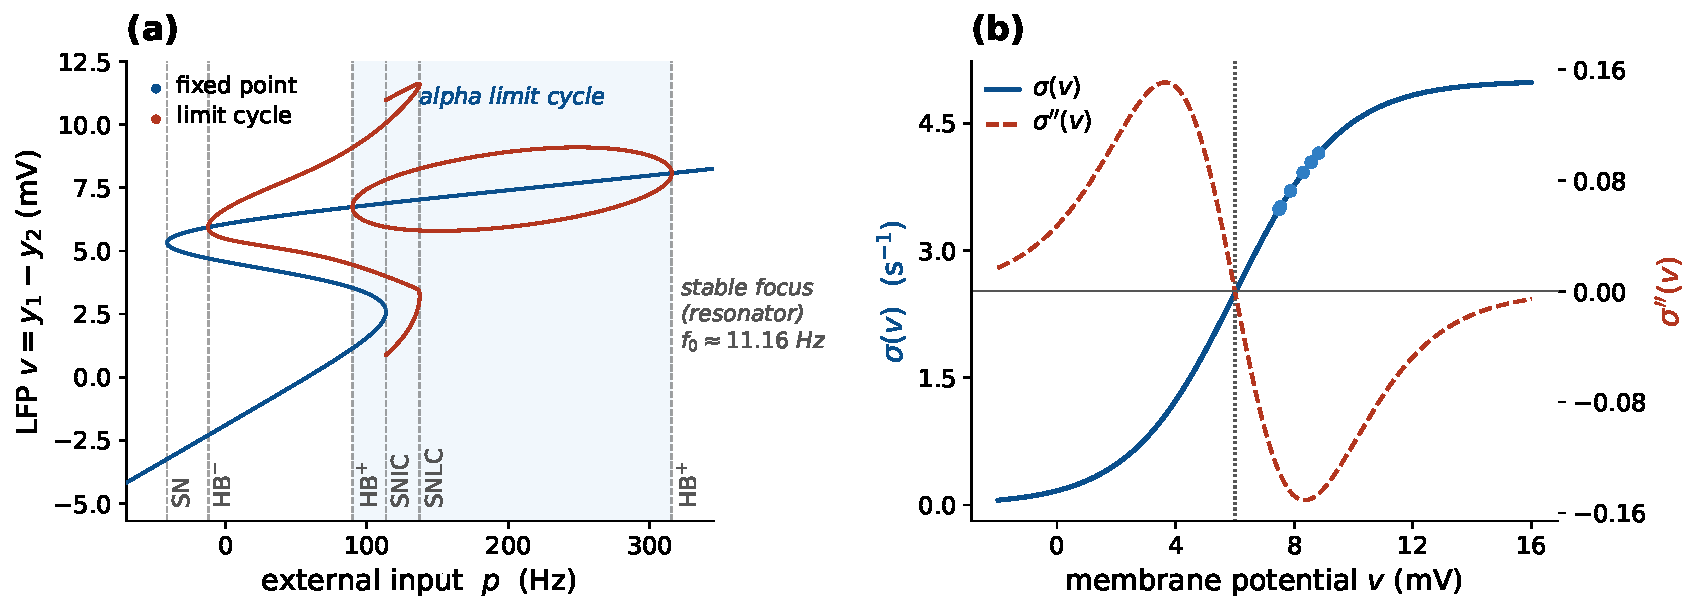
\includegraphics[width=\textwidth]{fig_bifurcation_sigmoid.pdf}
\caption{\textbf{The Jansen--Rit operating regime: bifurcation and sigmoid curvature.}
\emph{(a)} JR bifurcation diagram from numerical continuation---the LFP $v=y_1-y_2$ along
the fixed-point branch (blue) and the min/max of the limit-cycle branches (red) vs.\
external input $p$, with \emph{solid} stable and \emph{faded} unstable. The alpha limit
cycle (shaded) is bounded by a saddle-node-on-invariant-circle (SNIC, $p\!\approx\!114$)
and the supercritical Hopf ($p\!\approx\!315$, $f_0\!\approx\!11.1$~Hz); beyond the Hopf the
fixed point is a stable \DIFdelbeginFL \DIFdelFL{focus---the near-critical resonator regime used throughout. The
column is a weakly-damped }\DIFdelendFL focus\DIFdelbeginFL \DIFdelFL{near \emph{both} bifurcations}\DIFdelendFL , \DIFdelbeginFL \DIFdelFL{so it resonates on either
approach---more slowly near }\DIFdelendFL the \DIFdelbeginFL \DIFdelFL{SNIC}\DIFdelendFL \DIFaddbeginFL \DIFaddFL{near-Hopf resonator used here}\DIFaddendFL . Further
codim-1 points are marked (saddle-node SN, Hopf HB$^{\pm}$, saddle-node of limit cycles
SNLC). \emph{(b)} The sigmoid $\Sig(v)$ and its curvature $\Sig''(v)$, which sets the
demodulation gain and vanishes at the inflection $v_0$. Dots mark the operating points
reached by the closed-loop model for the $p$ values used here.}
\label{fig:bif}
\end{figure}

The response at the envelope frequency is read out with a software lock-in
amplifier referenced to $\Omega$---a standard way to isolate the component of a signal
at one chosen frequency: multiply by sine and cosine at $\Omega$ and average, so
everything \emph{not} at $\Omega$ cancels and only the envelope-locked amplitude
survives. Concretely we multiply $v(t)$ by quadrature references and
integrate over a Hann-windowed measurement window to obtain the in-phase ($I$) and
quadrature ($Q$) components,
\begin{equation}
I=\frac{2}{\sum_k w_k}\sum_k w_k\,(v_k-\bar v)\cos\Omega t_k,\quad
Q=\frac{2}{\sum_k w_k}\sum_k w_k\,(v_k-\bar v)\sin\Omega t_k,\quad
A_\Omega=\sqrt{I^2+Q^2},
\label{eq:lockin}
\end{equation}
with $w$ a Hann window and $\bar v=\sum_k w_k v_k/\sum_k w_k$ the windowed mean.
For a pure tone $v=A\cos(\Omega t+\phi)$ the product-to-sum identity gives
$I\to A\cos\phi$ and $Q\to -A\sin\phi$, so $A_\Omega\to A$\DIFdelbegin \DIFdel{exactly---the }\DIFdelend \DIFaddbegin \DIFadd{; the }\DIFaddend factor
$2/\sum_k w_k$ is the normalization that returns the physical amplitude, and
$A_\Omega$ equals twice the magnitude of the windowed Fourier coefficient at
$\Omega$. \DIFdelbegin \DIFdel{The one subtlety is that out-of-band components must not }\DIFdelend \DIFaddbegin \DIFadd{Out-of-band components can }\DIFaddend leak into the estimate\DIFdelbegin \DIFdel{; the dangerous one is the }\DIFdelend \DIFaddbegin \DIFadd{, particularly the }\DIFaddend DC level of $v$ ($\bar v\!\sim\!8$~mV, far
larger than the demodulated signal). Over an exact integer number of
$\Omega$-periods $\sum_k w_k\cos\Omega t_k=0$ and there is no leakage, but in
general it is nonzero, so we subtract $\bar v$ explicitly; this makes the metric
\DIFdelbegin \DIFdel{exact for a tone and robust }\DIFdelend \DIFaddbegin \DIFadd{accurate }\DIFaddend down to the $10^{-8}$ level needed for the kHz
analysis (\S\ref{sec:khz}). The signed in-phase component $I$ alone recovers
$\half\Sig''(v^*)\varepsilon^2 m$ including its sign, which we use to verify the
curvature law (Fig.~\ref{fig:opp}).

\DIFdelbegin \DIFdel{Three auxiliary constructions support the main results. Throughout we contrast the
\emph{open-loop detector}---the }\DIFdelend \DIFaddbegin \DIFadd{We compare the \emph{open-loop detector}, the }\DIFaddend firing-rate sigmoid \DIFdelbegin \DIFdel{alone }\DIFdelend at a fixed
operating point $v^*$ \DIFdelbegin \DIFdel{, with no recurrence---against }\DIFdelend \DIFaddbegin \DIFadd{without recurrence, with }\DIFaddend the \emph{closed-loop} column, the full recurrent
Jansen--Rit with its feedback. The open-loop detector passes the two-tone field through
$\Sig$ at $v^*$ and applies Eq.~\eqref{eq:lockin}, isolating the pure demodulation law
(Figs.~\ref{fig:carrier},~\ref{fig:opp},~\ref{fig:khz}). The \emph{bifurcation
diagram} records the field-free min/max of $v$ vs.\ $p$, each run initialized at
its fixed point plus a small kick. The \emph{two-dimensional map} evaluates
$A_\Omega$ over an ($\Omega,p$) grid. We verify the mechanism three ways: the
square law ($A_\Omega$ vs.\ $\varepsilon$ on a well-damped focus, expecting a
log--log slope of $2$); a linearization control (replacing $\Sig$ in
Eq.~\eqref{eq:jr0} by its tangent at $v^*$, which must abolish the $\Omega$
response); and a check of $\Sig',\Sig''$ against finite differences. All code is
openly available (see \emph{Code and data availability}).

\subsection{Laminar two-band model (LaNMM)}
We complement the single-column analysis with simulations of the laminar neural
mass model (LaNMM) of \S\ref{sec:nmm}. We integrate the full 28-variable column
\cite{ruffini2025cfc,sanchezTodo2023}, with the field entering exactly as in the single
JR \DIFdelbegin \DIFdel{column---as }\DIFdelend \DIFaddbegin \DIFadd{column, as }\DIFaddend a membrane polarization added inside the sigmoid argument of the target
population,
\begin{equation}
\varphi_X(t)=\Sig\!\big(v_X(t)+s(t)\big),\qquad X\in\{P_1,P_2\},
\label{eq:lanmm_drive}
\end{equation}
with $s(t)$ the AM or two-tone field of \S\ref{sec:coupling} (amplitude $\varepsilon$ in
mV, beat $\Omega=2\pi\Delta f$, carrier $\omega_c=2\pi f_c$) and all three external drives
held flat at their baselines (Fig.~\ref{fig:lanmm_setup}). \DIFdelbegin \DIFdel{Coupling the field this way,
rather than as a }\DIFdelend \DIFaddbegin \DIFadd{A }\DIFaddend perturbation of an external
input \emph{rate} \DIFdelbegin \DIFdel{, matters for more than
tidiness: a rate cannot go negative, so a rate-coupled AM drive must be clipped }\DIFdelend \DIFaddbegin \DIFadd{would require clipping }\DIFaddend at zero
once its excursion exceeds the baseline, and a hard clip is a half-wave rectifier---a
diode detector placed upstream of the sigmoid, which would inject a line at $\Delta f$
into the drive before the population nonlinearity ever saw it. A signed membrane
polarization carries no such constraint and none is applied. Because the LaNMM and JR
sigmoids share the voltage scale $1/\rho\approx1.8$~mV, $\varepsilon$ is directly
comparable between the two models. Integration is a vectorized fixed-step RK4
($\Delta t=10^{-4}$~s) advancing the whole parameter grid simultaneously, as in the JR
sweeps. In place of the lock-in (Eq.~\eqref{eq:lockin}) we read the
alpha-band ($8$--$12$~Hz) power of the $P_1$ and $P_2$ membrane potentials as the mean
squared magnitude of the Hann-windowed FFT over the band, in arbitrary units, over a
post-transient window, a phase-agnostic measure suited to the entrainment regime, where
lock-in phase slips would otherwise complicate the read-out. Two sweeps probe the column: an amplitude--beat sweep over
$(\varepsilon,\Delta f)$ at fixed carrier (the Arnold tongue), and a carrier--beat sweep
over $(f_c,\Delta f)$ at fixed $\varepsilon$, built on the LaNMM module of
\cite{ruffini2025cfc}. The maps
(Figs.~\ref{fig:lanmm_p2},~\ref{fig:lanmm_p1}) show the \emph{signed} stimulation-induced
change, alpha power minus the unstimulated ($\varepsilon=0$) baseline, on a zero-centered
scale; over most of the $P_1$-driven grids the change is negative. For the
alpha resonance we instead drive the deep $P_1$ loop directly and sweep its input against
$\Delta f$, reading the lock-in (Eq.~\eqref{eq:lockin}) of $v_{P_1}$ at $\Delta f$.

\subsection{Exact next-generation mean field (NMM2 PING)}
We test the mechanism in the exact next-generation mean field (NMM2, \S\ref{sec:nmm}),
following the Rosetta Stone formulation of \cite{ruffini2025rosetta} (which places the
Montbri\'o--Paz\'o--Roxin reduction \cite{montbrio2015} on a common footing with the JR
and LaNMM models used here), where the firing-rate nonlinearity is the derived MPR
dynamics of Eq.~\eqref{eq:mpr} rather than a postulated sigmoid. We use a two-population
excitatory--inhibitory (PING) motif \cite{ruffini2021nmm2,clusella2023,ruffini2025rosetta}:
each population $\alpha\in\{E,I\}$ is an MPR mean field (firing rate $r_\alpha$, mean
potential $v_\alpha$) with membrane time $\tau_\alpha$, coupled through second-order
synapses,
\begin{equation}
\begin{aligned}
\tau_E\dot r_E&=\Delta/(\pi\tau_E)+2r_Ev_E, &\quad
\tau_E\dot v_E&=v_E^2+\bar\eta-(\pi\tau_E r_E)^2+\tau_E C\,(s_E-s_I)+I_E(t),\\[2pt]
\tau_I\dot r_I&=\Delta/(\pi\tau_I)+2r_Iv_I, &\quad
\tau_I\dot v_I&=v_I^2+\bar\eta-(\pi\tau_I r_I)^2+\tau_I C\,(s_E-2s_I),
\end{aligned}
\label{eq:nmm2-ping}
\end{equation}
with second-order synaptic activations $s_E=\hat K_a[r_E]$ (excitatory, time constant
$\tau_a$) and $s_I=\hat K_g[r_I]$ (inhibitory, $\tau_g$), each obeying the same
critically-damped operator as the JR synapse, $\tau^2\ddot s+2\tau\dot s+s=r$; here $C$
is the global synaptic gain and the weights $(A_{ee},A_{ei},A_{ie},A_{ii})=(1,1,1,2)$
set the E and I \DIFdelbegin \DIFdel{rows---i.e.\ }\DIFdelend \DIFaddbegin \DIFadd{rows: }\DIFaddend the $E$ membrane sees $C\,(s_E-s_I)$ and the $I$ membrane
$C\,(s_E-2s_I)$, the only asymmetry being the doubled $I\!\to\!I$ weight $A_{ii}=2$. The common background drive $\bar\eta$ \DIFdelbegin \DIFdel{---the same in both
populations, with no separate input current---is }\DIFdelend \DIFaddbegin \DIFadd{is }\DIFaddend the bifurcation parameter: raising it
past a supercritical Hopf at $\bar\eta_H=1.110$ opens a gamma limit cycle (the gamma
counterpart of the JR alpha Hopf). The applied field enters the excitatory voltage equation
as a current-like forcing, $I_E(t)=P\,E(t)$ in the convention of the exact mean field
\cite{ruffini2021nmm2}, with the dipole coupling $P$ instantaneous, as two genuine tones at
$f_c\mp\Delta f/2$ (carrier $f_c=300$~Hz, envelope $\Delta f$ swept through the gamma band)
of amplitude $A_f$ in the dimensionless MPR units of $v_E$. The E membrane $\tau_E\dot v_E$
integrates this forcing into the carrier-frequency excursion $A_f/(\omega\tau_E)$ that the
exact quadratic $v_E^2$ term rectifies, with no postulated sigmoid; the PING as run is
therefore \DIFdelbegin \DIFdel{the somatic door of Eq.~\eqref{eq:doors} }\DIFdelend \DIFaddbegin \DIFadd{computes membrane access }\DIFaddend with $\tau_m=\tau_E$\DIFdelbegin \DIFdel{, computed rather
than assumed}\DIFdelend . We
integrate with fixed-step RK4 ($\Delta t=0.05$~ms) and read out the lock-in
(Eq.~\eqref{eq:lockin}) of $r_E$ at $\Delta f$ over the $(\Delta f, \bar\eta)$ plane.
Parameters (Rosetta Stone PING \cite{ruffini2025rosetta}): $\Delta=1$, global coupling
$C=15$, $\tau_E=15$, $\tau_I=7.5$, $\tau_a=10$, $\tau_g=2.5$~ms, with $\bar\eta$ swept
through the supercritical Hopf at $\bar\eta_H=1.110$ ($f_0=54.0$~Hz), located by bisection
on the leading eigenvalue of the mean-field Jacobian. \DIFaddbegin \DIFadd{The simulations retain these
finite membrane times; Eq.~\eqref{eq:slow_synapse} characterizes the fast-membrane limit.
}\DIFaddend

Two parameters reach this gamma Hopf, and we use both as criticality knobs---just as the
external drive $p$ and the coupling $C$ both reach the JR alpha Hopf. The background drive
$\bar\eta$ (above) is swept for the resonance map (Fig.~\ref{fig:nmm2_map}); the global
coupling $C\,(\equiv J)$ is swept for the J-curve (Fig.~\ref{fig:nmm2_jcurve}): we vary
$J$ at fixed $\bar\eta$ toward the gamma Hopf $J^*$ (located by bisection on the leading
Jacobian eigenvalue) and read the lock-in peak of $r_E$ over $\Delta f$. Unlike the JR
J-curve, \emph{no operating-point pinning is needed}: at this carrier the generated
difference-frequency source is operating-point independent to about $1\%$
(\S\ref{sec:dynamic}), so sweeping $J$ changes the damping $\gamma$ and the modal
projections but not the source, and the gain is read as the response per unit source.

\subsection{QIF spiking network (microscale of NMM2)}\label{sec:qif-methods}
NMM2 is the exact mean field of an all-to-all network of QIF neurons
\cite{montbrio2015,ruffini2025rosetta,clusella2023}, so we integrate that network directly
to test the prediction at the spike level (\S\ref{sec:qif}): $N=8000$ QIF neurons per
population, parameters identical to the PING mean field (Eq.~\eqref{eq:nmm2-ping}),
excitabilities $\eta_j\sim$ Lorentzian$(\bar\eta,\Delta)$ sampled by deterministic
quantiles, second-order synapses driven by the empirical population rates, and a genuine
two-tone field entering the excitatory membranes. Spiking and threshold dynamics are
where the AM surrogate and the physical waveform cannot be assumed equivalent beyond
perturbation theory, so this run uses two tones throughout. The bifurcation parameter is the common
background drive $\bar\eta$, with the gamma Hopf at $\bar\eta_H=1.110$ ($f_0=54.0$~Hz)
from the mean-field Jacobian; the spiking network shows the same threshold and an
autonomous $f_0\!\approx\!53$~Hz, with no finite-size offset to explain. The carrier is
$f_c=300$~Hz and the field amplitude $A_f=35$. Because
this is a \emph{gamma} circuit, the TI beat $\Delta f$ is set in the gamma band:
$\Delta f=55$~Hz \emph{near} the forced gamma resonance ($\bar\eta=0.85$, below the Hopf) and
$\Delta f=42$~Hz in the oscillatory regime ($\bar\eta=1.5$, above the Hopf)---a detuning of
$\approx$11~Hz below the autonomous $f_0\!\approx\!53$~Hz that places the beat outside the
$1{:}1$ Arnold tongue, so the above-Hopf response is gating, not entrainment
(\S\ref{sec:vocab}). The network is integrated with Euler steps of $0.0025$~ms, settled for $800$~ms (over
four relaxation times at $\bar\eta=0.85$, where the mean-field relaxation time is
$176$~ms) and measured over an integer number of beat cycles, $44$ at $55$~Hz and $34$ at
$42$~Hz ($800$ and $810$~ms), so that the finite-window bias of phase statistics
vanishes. Envelope-locked timing is quantified by the quadrature lock-in $A_\Omega$ of
$r_E(t)$ at $\Delta f$, reported as the modulation depth $A_\Omega/\langle r_E\rangle$ (a
stable measure; the off$\to$on lock-in ratio would divide by the field-free floor), and
per neuron by the pairwise phase consistency of each neuron's spike phases at $\Delta f$
\cite{vinck2010}, which is unbiased in the spike count, over neurons with at least ten
spikes in the window. Halving the time step changes the lock-in and the pooled vector
strength by under $1\%$; doubling the spike-detection threshold changes the lock-in by
about $1\%$ and the mean rate by $2\%$, but the pooled vector strength in the forced
regime by about $45\%$, so phase concentration, unlike rate modulation, is sensitive to
how spike times are defined.

\subsection{Coupling sweeps, timing, and the tACS control (Jansen--Rit)}
The coupling sweeps of Figs.~\ref{fig:jcurve} and~\ref{fig:timing}, and the transcranial
alternating-current stimulation (tACS) control of Fig.~\ref{fig:tacs}, use the single JR
column with the operating point $v^*$ pinned: for
each global connectivity $C$ we solve the field-free fixed-point relation analytically
for the external drive $p(C)$ that holds $v^*$ (hence $\Sig''(v^*)$) fixed, vary $C\,(=J)$
toward the alpha Hopf, and read $\gamma,\omega_0$ from the $6\times6$ Jacobian. The field
is the AM surrogate of Eq.~\eqref{eq:amsur} for TI (Fig.~\ref{fig:jcurve}; AC lock-in vs DC mean
rate for Fig.~\ref{fig:timing}) or a direct in-band sinusoid $s(t)=\varepsilon\cos\Omega t$
($\varepsilon=0.1$~mV) for the tACS control (Fig.~\ref{fig:tacs}), each read out by the
lock-in of $v$ at $\Delta f$.

\subsection{Vocabulary: forced response, entrainment, and gating}
``Entrainment'' is used in several senses, so we fix three terms. \emph{Forced response}
is the driven, non-autonomous case below the Hopf, quantified by the lock-in amplitude at
the beat $\Delta f$ (Eq.~\eqref{eq:lockin}). \emph{Entrainment} is reserved for its
dynamical-systems meaning, frequency capture of a \emph{self-sustained} oscillator
\cite{pikovsky2001}; in the maps we screen for it with the dominance criterion
$|f_{\rm out}-\Delta f|<0.3$~Hz on the dominant output frequency, a necessary but not
sufficient condition for capture. \emph{Gating} is amplitude modulation of a persisting rhythm without
frequency capture \cite{canolty2010,tort2010}. Capture and gating are dynamically different, and the same word would otherwise cover
both; Appendix~\ref{sec:vocab} gives the metrics and the Arnold-tongue protocol.

\section{Results}
Two rungs of the modeling ladder carry the evidence: the single Jansen--Rit column
(closed form, memoryless detector) and the exact next-generation mean field (NMM2, the
nonlinearity derived rather than postulated) with its spiking network. Each shows the same
pair, quadratic difference-frequency generation followed by near-Hopf amplification, with
different detector coefficients. Two mesoscale signatures follow: the network's own
coupling sets the gain at fixed generated drive (the $J$-curve, \S\ref{sec:jcurve}), and
the resonance amplifies the envelope-locked modulation far more than the mean rate
(\S\ref{sec:timing}), which the QIF network tests at the spike level. The laminar two-band
column, at carriers of $25$--$80$~Hz and drives up to $3$~mV, is an extension
(App.~\ref{app:lanmm}).

\subsection{The Jansen--Rit sigmoid demodulates: an alpha line from a carrier-only input}
The system is oriented by Fig.~\ref{fig:bif}: a clean supercritical Hopf at
$p\!\approx\!315$ with $f_0\!\approx\!11.1$~Hz, and a sigmoid whose curvature peaks
well off the inflection, so the closed-loop operating points sit where $\Sig''$ is
large. The core result is Fig.~\ref{fig:demod}: an input with no spectral power in
the alpha band (lines only at $f_c$ and $f_c\pm\Delta f$) produces a clean
$\sim$11~Hz output oscillation locked to the envelope, with a strong alpha peak in
the output spectrum absent from the input.

\begin{figure}[t!]
\centering
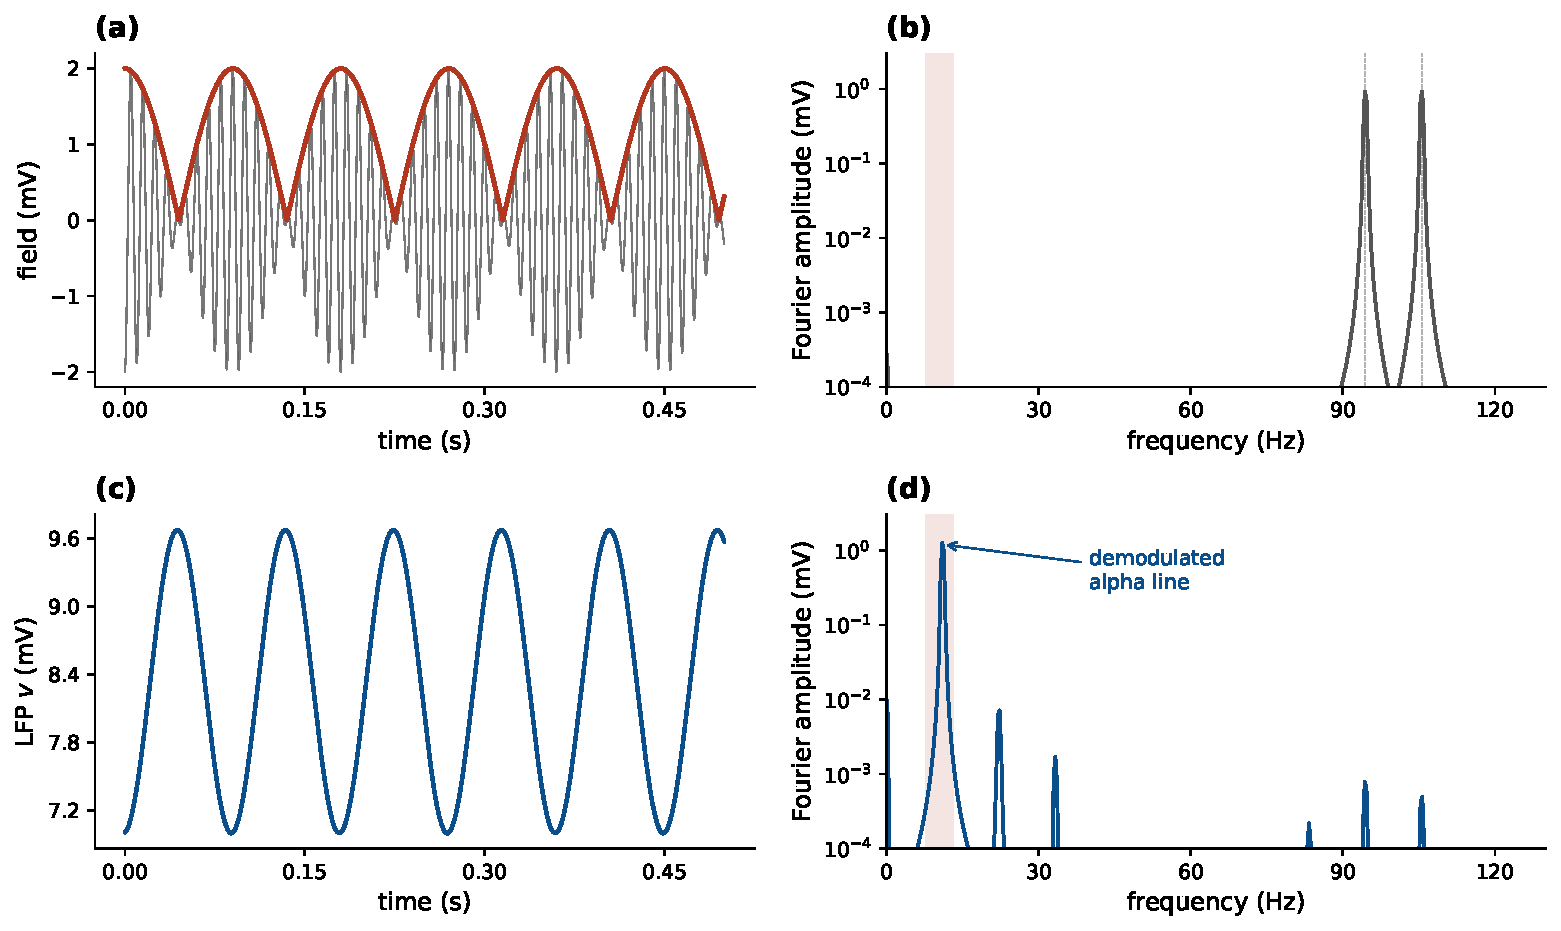
\includegraphics[width=\textwidth]{fig_demodulation_twotone.pdf}
\caption{\textbf{An alpha rhythm is synthesized from a two-tone TI input (Jansen--Rit
below Hopf).} The field is the physical TI waveform, two equal tones at
$f_{1,2}=f_c\mp\Delta f/2$, not the amplitude-modulated surrogate. \emph{(a)} The field
$s(t)$ and its envelope $A(t)=2\varepsilon|\cos(\Omega t/2)|$---a rectified cosine, not a
sinusoid; it is $A^2$ that is sinusoidal at $\Omega$ (\S\ref{sec:coupling}).
\emph{(b)} The input amplitude spectrum has lines only at $f_1$ and $f_2$ ($94.45$ and
$105.55$~Hz, $\Delta f=11.1$~Hz) and no third line at the carrier; in the alpha band
(shaded) it is $1.6\times10^{-8}$ of the tone amplitude, finite-window leakage rather than
physical power.
\emph{(c)} The output $v=y_1-y_2$ oscillates at the envelope frequency.
\emph{(d)} The output spectrum has a strong peak at the beat, $11.1$~Hz,
synthesized by the sigmoid and absent from the input.}
\label{fig:demod}
\end{figure}

\subsection{Near the Hopf, the demodulated beat drives a sharp resonance}
The resonance is quantified in Fig.~\ref{fig:res}. In the
fixed-point regime ($p>315$, a stable focus) the response is a Lorentzian centered at
$f_0$ whose height grows monotonically as the Hopf is approached
($0.23\!\to\!0.43\!\to\!0.70$~mV; Fig.~\ref{fig:res}), i.e.\ gain $\propto1/\gamma$. This
is genuine forced gain: with no drive the focus is silent at $\Omega$, so all power at
$\Omega$ is synthesized by the demodulating nonlinearity and amplified by the recurrent
loop. Above the Hopf ($p<315$) the
column free-runs at $f_0$ and the demodulated drive instead phase-locks that autonomous
alpha within a $1{:}1$ Arnold tongue; because lock-in amplitude at $\Omega$ then conflates
the driven response with the free-running cycle, we characterize that regime with the
output frequency $f_{\rm out}$ rather than the lock-in amplitude (Fig.~\ref{fig:entrain}).

\begin{figure}[t!]
\centering
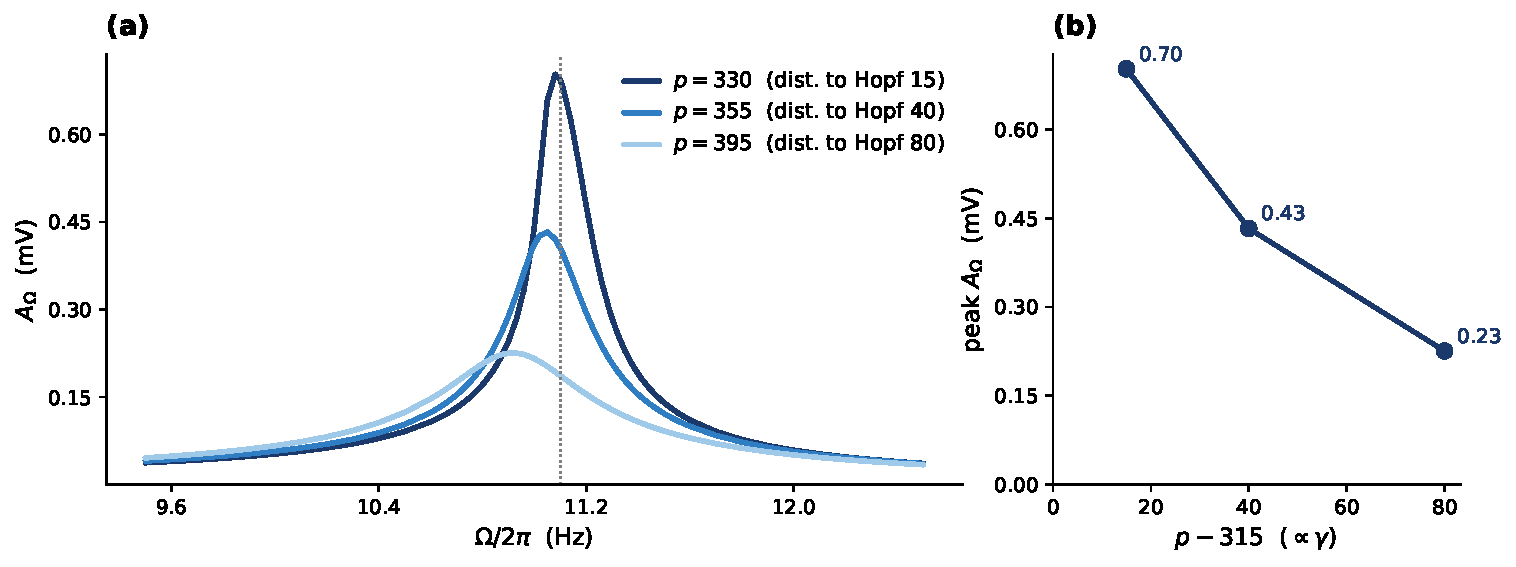
\includegraphics[width=\textwidth]{fig_resonance.pdf}
\caption{\textbf{The demodulated beat drives a resonance that sharpens toward the Hopf (Jansen--Rit).}
Fixed-point regime ($p>315$, stable focus): lock-in response at $\Omega$ vs.\ envelope
frequency ($\varepsilon=0.3$~mV). \emph{(a)} The demodulated drive forces a Lorentzian
resonance at $f_0\!\approx\!11.1$~Hz whose peak redshifts slightly as the damping grows
($\omega_{\rm peak}=\sqrt{\omega_0^2-2\gamma^2}$; $11.08\!\to\!10.93$~Hz across the three
curves); the response carries no power at $\Omega$ in the absence of drive, so this is
genuine forced gain. \emph{(b)} The peak height grows as the Hopf is
approached ($p\!\to\!315$, distance to Hopf $\to0$). Three points cannot establish a power
law; the $1/\gamma$ scaling is quantified over a decade, together with its saturation, in
Fig.~\ref{fig:jcurve}(c). The complementary above-Hopf regime, where the demodulated drive
\emph{entrains} the autonomous alpha within a $1{:}1$ Arnold tongue, is characterized with
the appropriate observable (output frequency $f_{\rm out}$, not lock-in amplitude) in
Fig.~\ref{fig:entrain}.}
\label{fig:res}
\end{figure}

\subsection{Carrier independence and the kHz roll-off}
At fixed post-coupling polarization the demodulated response is flat across the
carrier band, for both the open-loop detector and the closed-loop column near the Hopf
(Fig.~\ref{fig:carrier}). As a function of
the \emph{applied} field, by contrast, the membrane low-pass makes the response roll
off as $1/f_c^2$ above the corner (Fig.~\ref{fig:khz}): passive somatic demodulation
is suppressed four to six orders of magnitude at kHz \DIFdelbegin \DIFdel{, whereas a fast element
($\tau\!\approx\!0.2$~ms ) retains an appreciable response into the kHz band}\DIFdelend \DIFaddbegin \DIFadd{in the $16$~ms access model,
whereas the assumed $0.2$~ms response retains appreciable carrier access}\DIFaddend .

\begin{figure}[t!]
\centering
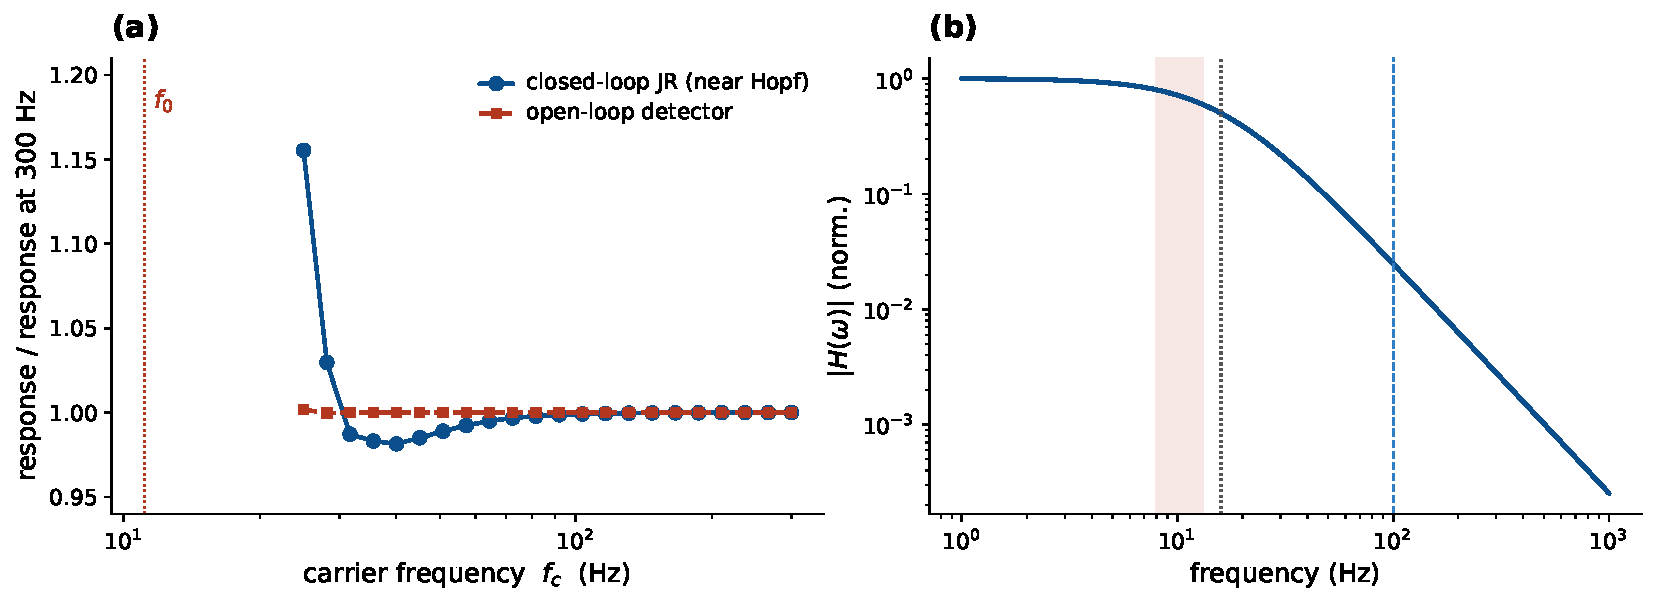
\includegraphics[width=\textwidth]{fig_carrier_independence.pdf}
\caption{\textbf{The demodulated response is carrier-independent at fixed polarization (Jansen--Rit).} \emph{(a)} The demodulated response is
flat across carrier frequency $f_c=25$--$300$~Hz, both for the open-loop detector
(exactly, by Eq.~\eqref{eq:demod}) and for the closed-loop JR near the Hopf (which
adds $\sim$60$\times$ resonant gain); deviations appear only as $f_c$ approaches
the natural band. \emph{(b)} The second-order-synapse low-pass $|H_s(\omega)|/|H_s(0)|$
passes the envelope ($\sim$0.7) and suppresses the $100$~Hz carrier ($\sim$2.5\%). Dotted line: synaptic corner $a/2\pi\!\approx\!16$~Hz; shaded band: envelope ($8$--$13$~Hz); dashed line: $100$~Hz carrier.}
\label{fig:carrier}
\end{figure}

\DIFdelbegin \DIFdel{To pre-empt the objection that the demonstration runs only at $100$~Hz, we }\DIFdelend \DIFaddbegin \DIFadd{We also }\DIFaddend drive the full recurrent column with a \DIFdelbegin \DIFdel{genuine }\DIFdelend kHz field, passing it through
an explicit membrane low-pass (an extra first-order state, time constant $\tau$) for
each coupling route before it reaches the sigmoid. The
column demodulates and resonates at the recovered alpha \DIFdelbegin \DIFdel{well into the kHz band when
the nonlinearity sits at a fast element ($\tau\!\approx\!0.2$}\DIFdelend \DIFaddbegin \DIFadd{in the fast-access case
($\tau=0.2$}\DIFaddend ~ms), \DIFdelbegin \DIFdel{exactly }\DIFdelend as
Eq.~\eqref{eq:khz} predicts (Fig.~\ref{fig:khz_direct}a). Driving the fast-element route
with two \emph{genuine} tones at $f_{1,2}=1994.54$ and $2005.46$~Hz, centered near
$2$~kHz and beating at $10.91$~Hz, the input carries $2.2\times10^{-13}$ of its spectral
amplitude in the $8$--$14$~Hz band, i.e.\ none, while the output carries a line at the
beat
(Fig.~\ref{fig:khz_twotone}), with the attenuation set by the analytic
$|H_m|^2\!=\!0.137$ at $2$~kHz for $\tau=0.2$~ms. The kHz claim therefore rests on the
\DIFdelbegin \DIFdel{physical waveform , not on an extrapolation from the AM surrogate. That the bare unmodulated kHz carrier is
itself
weakly effective---the premise of TI's focality---is consistent with the limited
sensitivity of hippocampal network oscillations }\DIFdelend \DIFaddbegin \DIFadd{two-tone waveform under the specified access assumption. The anatomical route is
not determined by this calculation. Limited sensitivity }\DIFaddend to unmodulated kHz fields
\DIFaddbegin \DIFadd{has been reported in hippocampal network oscillations }\DIFaddend \cite{esmaeilpour2020}.

\subsection{The nonlinearity is the detector: the
\texorpdfstring{$\Sig''$}{sigma''} curvature law and its controls}\label{sec:results-curvature}
The signed open-loop response tracks $\half\Sig''(v^*)\varepsilon^2 m$ across the
operating range, vanishing and reversing sign at the inflection $v_0$
(Fig.~\ref{fig:opp})---demodulation is the sigmoid-curvature term of
Eq.~\eqref{eq:demod}, and the closed-loop operating points sit where $\Sig''$ is large
and negative.

\begin{figure}[t!]
\centering
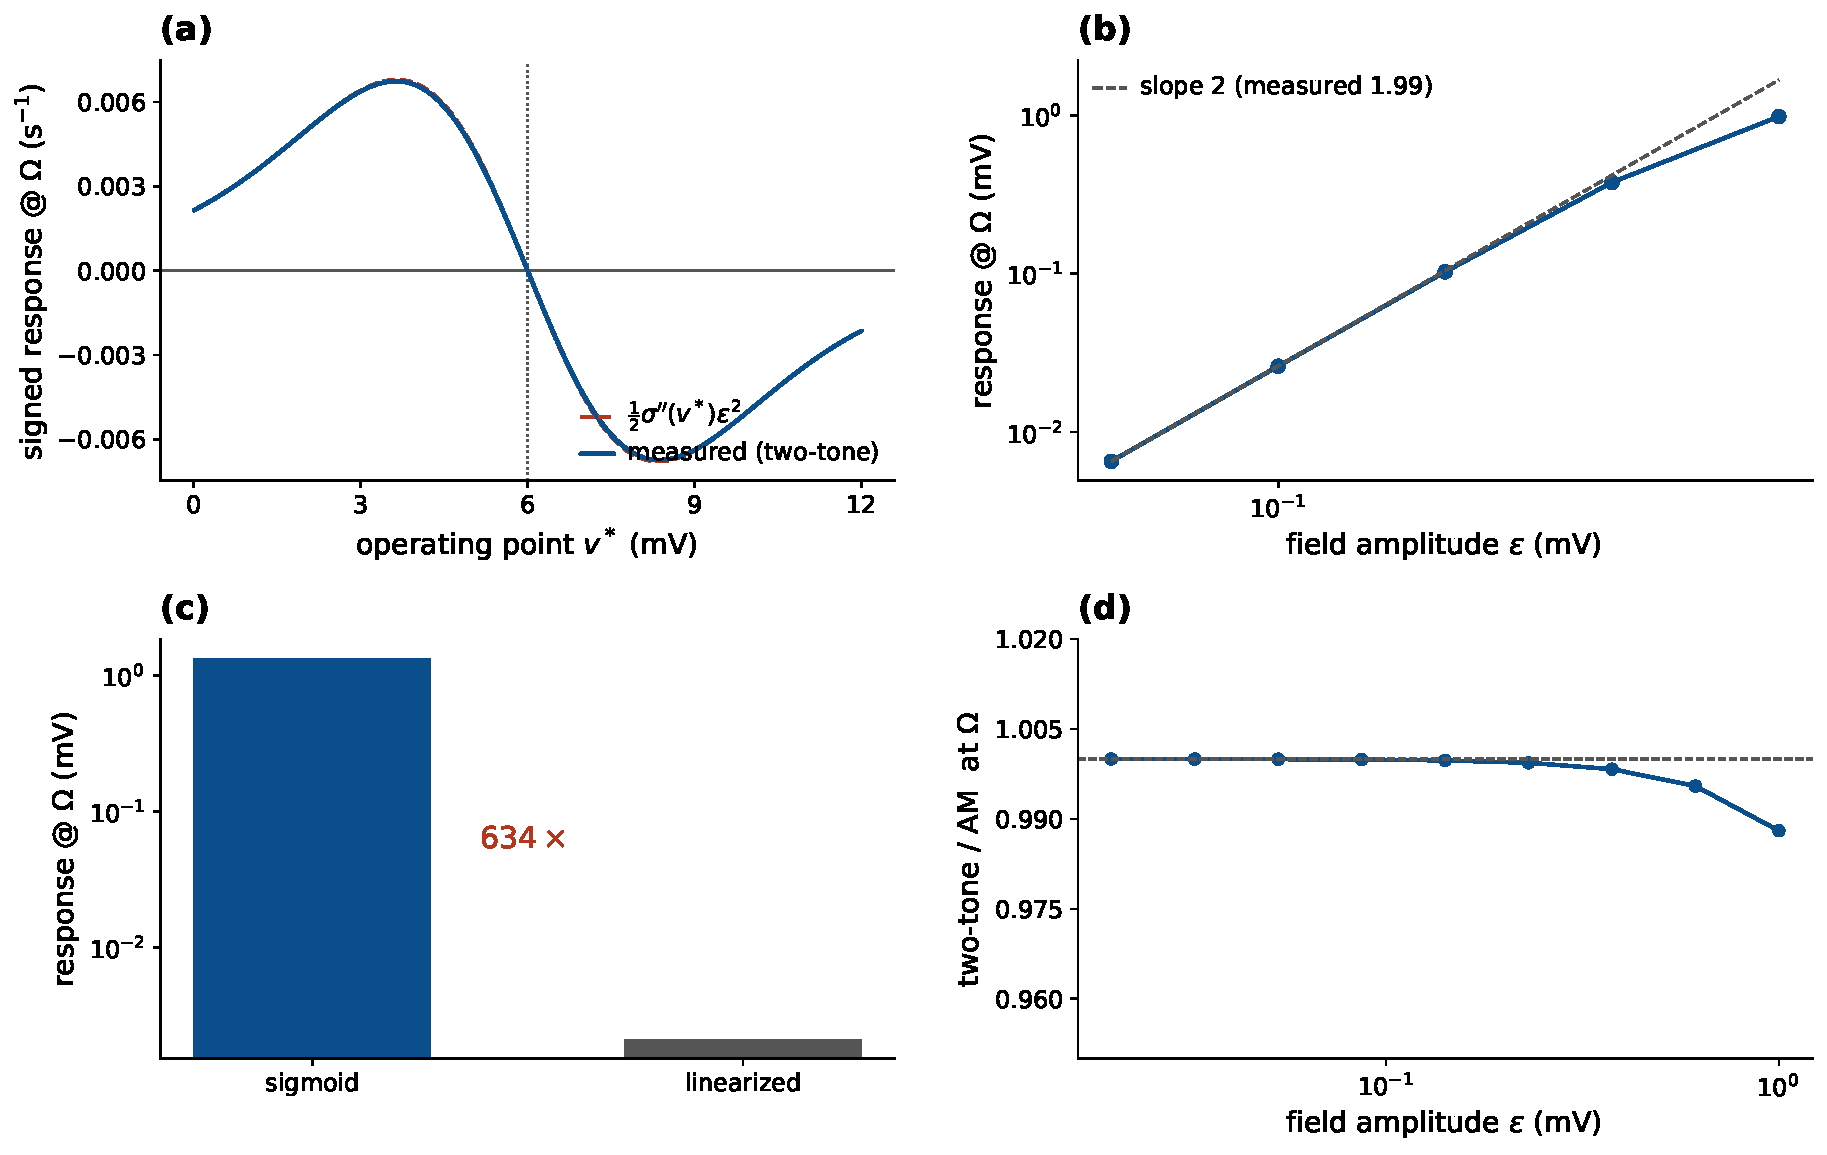
\includegraphics[width=\textwidth]{fig_curvature_twotone.pdf}
\caption{\textbf{The curvature law, the square law, and the surrogate control
(Jansen--Rit, genuine two tones).} \emph{(a)} The signed open-loop response tracks
$\half\Sig''(v^*)\varepsilon^2$ across the operating range (maximum deviation $0.9\%$),
vanishing at the inflection $v_0$ and reversing sign across it. The mechanism is
sign-agnostic: $\Sig''$ sets sign and phase while $|\Sig''|$ sets gain, so the resonance
picture is unchanged up to an overall sign in the $\Sig''>0$ lobe, which this sweep spans.
The sign flip is itself a prediction (\S\ref{sec:predictions}). \emph{(b)} The closed-loop
response scales as $\varepsilon^2$, measured slope $1.99$. \emph{(c)} Replacing the
field-receiving sigmoid by its tangent collapses the response $634\times$. \emph{(d)}
Surrogate control: the two-tone/AM ratio at $\Omega$ approaches $1$ as
$\varepsilon\!\to\!0$ ($1.0000$ at $0.02$~mV, $0.988$ at $1$~mV), licensing the AM
surrogate for the dense sweeps of Fig.~\ref{fig:jcurve}, which read only that component,
and for nothing else.}
\label{fig:opp}
\end{figure}

Two controls test the proposed source of the beat component (Fig.~\ref{fig:opp}b,c): the response scales as
$\varepsilon^2$ at small drive (measured log--log slope $1.99$ against the
predicted $2$), and replacing the field-receiving sigmoid by its linearization
collapses the response by $634\times$ ($1.34\!\to\!0.0021$~mV)---the nonlinearity is
the detector, and its curvature is the gain. A third panel checks the surrogate at one operating point: for the open-loop detector
at $v^*=8$~mV the two-tone and AM responses at $\Omega$ agree to within $10^{-4}$ at
$\varepsilon=0.02$~mV and to $1.2\%$ at $1$~mV (Fig.~\ref{fig:opp}d). On that basis the
dense perturbative sweeps below, which read only the $\Omega$ component, use the surrogate;
the comparison does not test the recurrent response near the Hopf, where the two
waveforms' different DC terms could shift the operating state.

\subsection{Exact mean-field confirmation: the NMM2 PING gamma generator}\label{sec:nmm2-results}
The JR column and the LaNMM both use the heuristic firing-rate sigmoid (NMM1). As a
third, independent test we move to the exact next-generation mean field (NMM2,
Eq.~\eqref{eq:mpr}), where the demodulating nonlinearity is the \emph{derived}
quadratic $v^2$ term rather than a postulated curve. We drive the two-population E--I PING motif of
Eq.~\eqref{eq:nmm2-ping} (Methods)\DIFdelbegin \DIFdel{---a gamma generator that }\DIFdelend \DIFaddbegin \DIFadd{, which }\DIFaddend loses stability through a supercritical
Hopf \DIFdelbegin \DIFdel{(}\DIFdelend at $\bar\eta_H=1.110$, $f_0=54.0$~Hz\DIFdelbegin \DIFdel{), the gamma
counterpart of the JR alpha Hopf---with the }\DIFdelend \DIFaddbegin \DIFadd{, with the }\DIFaddend two-tone field entering the
excitatory current,
so the carrier is rectified by the exact $v_E^2$ term.

Driving with a two-tone TI field (carrier $f_c=300$~Hz, envelope $\Delta f$ swept through
the gamma band) and locking in the excitatory rate $r_E$ at $\Delta f$ reproduces the
\DIFdelbegin \DIFdel{whole picture }\DIFdelend \DIFaddbegin \DIFadd{generation and amplification of the beat }\DIFaddend (Figs.~\ref{fig:nmm2_res},~\ref{fig:nmm2_map}). Below the Hopf the
response is a forced resonance at the gamma frequency whose height grows as the
bifurcation is \DIFdelbegin \DIFdel{approached---the }\DIFdelend \DIFaddbegin \DIFadd{approached, following the }\DIFaddend $1/\gamma$ gain of Eq.~\eqref{eq:gain}; above it the
demodulated drive entrains the autonomous gamma. The two-dimensional map traces a
ridge at $\Delta f\!\approx\!f_0$ that intensifies through the Hopf. \DIFdelbegin \DIFdel{Unlike the
static-sigmoid models, the resonant frequency itself \emph{shifts with the operating
point}---the ridge is diagonal, not vertical---a direct signature of the
dynamic, state-dependent transfer of the exact theory }\DIFdelend \DIFaddbegin \DIFadd{Compared with the
JR sweep shown here, the NMM2 resonant frequency shifts appreciably with the
operating point, producing a diagonal ridge }\DIFaddend \cite{clusella2023}. That the beat is generated and resonantly amplified with the nonlinearity
\emph{derived} from QIF spiking dynamics, rather than assumed, shows the receiver behavior
is not an artifact of the heuristic sigmoid. The detector coefficient, however, is not the
sigmoid's: at this $300$~Hz carrier the population is on the fast side of its crossover,
and the generated source is the $v_E^2$ mixing of the carrier-frequency voltage excursion,
operating-point independent to about $1\%$ (\S\ref{sec:dynamic}, Fig.~\ref{fig:crossover}).

\begin{figure}[t!]
\centering
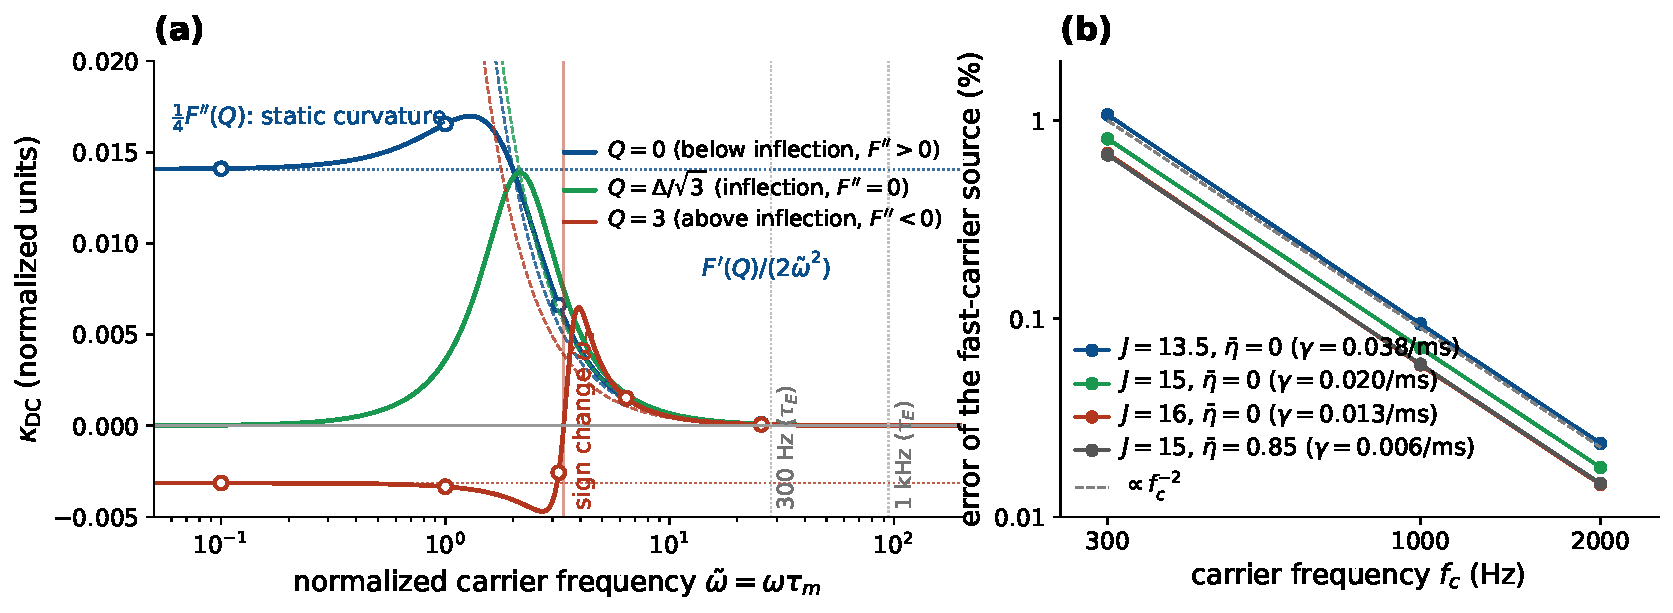
\includegraphics[width=\textwidth]{fig_mpr_crossover.pdf}
\caption{\textbf{Static curvature at slow carriers, slope at fast ones.} \emph{(a)}
Second-order DC rate shift of an uncoupled MPR population ($\Delta=1$, $\tau=1$) under a
current carrier, Eq.~\eqref{eq:crossover}, for operating points below, at and above the
inflection of $F(Q)$. Dotted: the static limit $\tfrac14F''$; dashed: the fast-carrier
limit $F'/(2\omega^2)$; circles: RK4 integrations at $a=0.05$ averaged over whole carrier
periods (relative error below $10^{-3}$). Above the inflection the sign changes at
$\omega_z$. The top axis converts $\omega\tau$ to a carrier frequency for
$\tau=\tau_E=15$~ms. \emph{(b)} PING of Eq.~\eqref{eq:nmm2-ping}: relative error of the
fast-carrier difference-frequency source against the exact second-order response at four
stable operating points ($\gamma$ the damping of the gamma mode), two tones centered at
$300$, $1000$ and $2000$~Hz.}
\label{fig:crossover}
\end{figure}

\begin{figure}[t!]
\centering
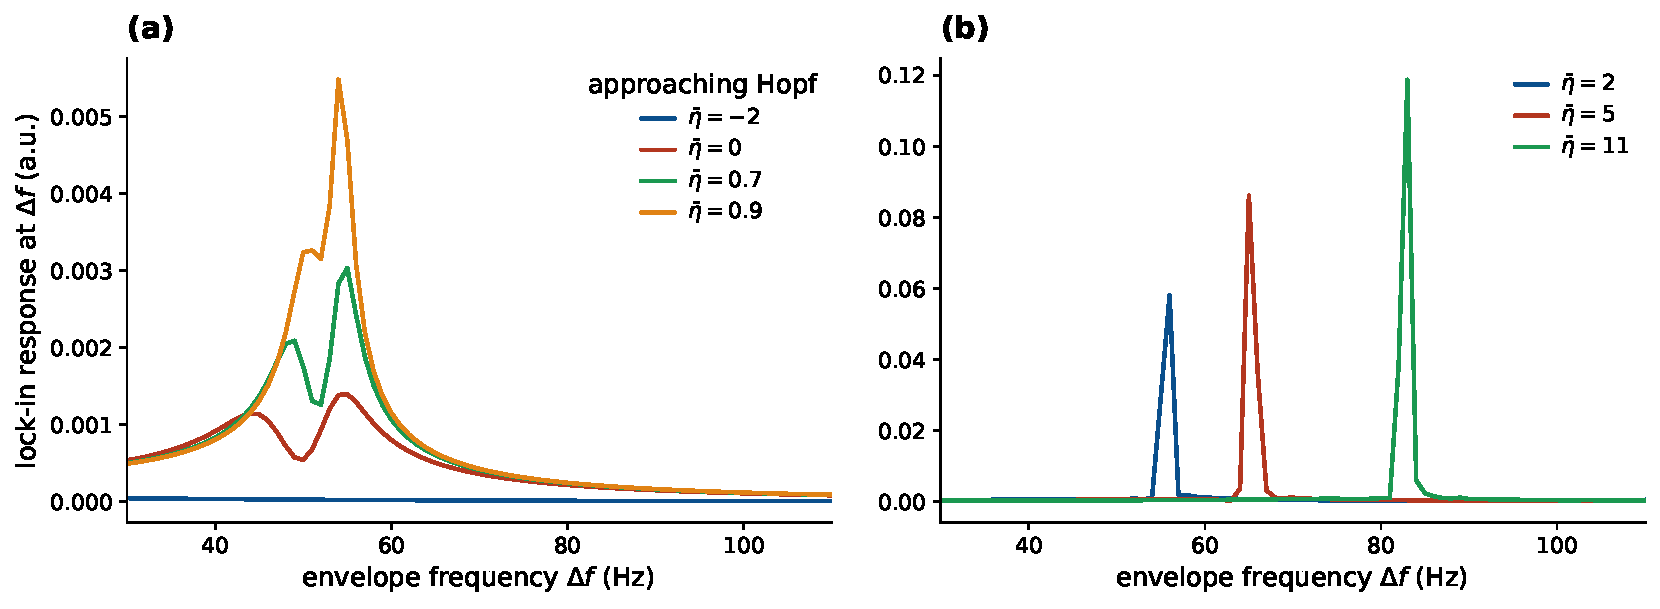
\includegraphics[width=\textwidth]{fig_nmm2_resonance_twotone.pdf}
\caption{\textbf{NMM2 PING gamma resonance (exact mean field, genuine two tones).}
Lock-in response of the excitatory rate $r_E$ at the envelope frequency $\Delta f$ under a
two-tone TI field (carrier $300$~Hz). \emph{(a)} (stable focus,
$\bar\eta<\bar\eta_H=1.110$) forced resonance at the gamma frequency
($f_0\!\approx\!54$~Hz), the peak growing $0.0014\!\to\!0.0030\!\to\!0.0055$ as the Hopf
is approached ($1/\gamma$ gain). \emph{(b)} (limit cycle,
$\bar\eta>\bar\eta_H$) entrainment of the autonomous gamma, the peak shifting
upward with $\bar\eta$ ($56\!\to\!65\!\to\!83$~Hz). The input carries no power at
$\Delta f$; the response is synthesized by the exact quadratic $v^2$ nonlinearity, with no
sigmoid anywhere in the model. Matched AM and two-tone drives agree at $\Omega$ to
$0.07\%$ well below the Hopf and to $4\%$ at $\bar\eta=0.9$, consistent with the JR
surrogate control (Fig.~\ref{fig:opp}d).}
\label{fig:nmm2_res}
\end{figure}

\subsection{What the mesoscale adds: coupling sets the gain at fixed detection}\label{sec:jcurve}
The resonance sweeps above drove the column toward the Hopf with the external input
$p$, but $p$ also shifts the operating point, entangling detection ($\Sig''$) with
amplification. \DIFdelbegin \DIFdel{The sharper, mechanistic statement is that the \emph{network coupling}
sets the gain on its own. In the JR column }\DIFdelend \DIFaddbegin \DIFadd{To isolate amplification, }\DIFaddend we vary the \DIFaddbegin \DIFadd{JR }\DIFaddend global connectivity $C$ \DIFdelbegin \DIFdel{---the
}\DIFdelend \DIFaddbegin \DIFadd{(}\DIFaddend coupling
strength $J$\DIFdelbegin \DIFdel{---and, for each $C$, }\DIFdelend \DIFaddbegin \DIFadd{) and }\DIFaddend solve analytically for the drive $p(C)$ that
\emph{pins} the operating point $v^*$, so the detection gain $\Sig''(v^*)$ and the
open-loop detector amplitude $A_{\rm open}=\half\Sig''(v^*)\varepsilon^2 m$ are held
exactly constant. As $C\!\to\!C^*$ (the Hopf, $C^*\!\approx\!137$) the damping
$\gamma\!\to\!0$, the demodulated response grows $\sim 30\times$ and the envelope
resonance sharpens (Fig.~\ref{fig:jcurve}a,b)\DIFdelbegin \DIFdel{---entirely }\DIFdelend \DIFaddbegin \DIFadd{, }\DIFaddend a network effect \DIFdelbegin \DIFdel{, }\DIFdelend since
detection is frozen and only $\gamma$ changes. The recovered gain
$A_\Omega/A_{\rm open}$ tracks $1/\gamma$ before saturating near criticality
(Fig.~\ref{fig:jcurve}c); driving the same column to the Hopf through the input $p$
rather than the coupling $C$ yields the same gain--$\gamma$ relation, so the
amplification depends only on the distance to criticality, not on which parameter
delivers it. All these sweeps stay on the stable-focus side ($\gamma>0$), approaching
the supercritical Hopf from below: the $1/\gamma$ growth is the forced-resonance
susceptibility of a damped network, not entrainment of an autonomous cycle. On the
other side of the bifurcation the column oscillates on its own, and the demodulated
drive instead phase-locks that limit cycle within an Arnold tongue
(Fig.~\ref{fig:entrain}; also the entrainment side of Fig.~\ref{fig:res} and the LaNMM
and NMM2 maps)\DIFdelbegin \DIFdel{---}\DIFdelend \DIFaddbegin \DIFadd{: }\DIFaddend $1{:}1$ frequency capture over a band that widens with drive,
quantified by the locking range rather than a diverging $1/\gamma$ gain, the two
coinciding only at onset. Because the drive is weak, on the autonomous side it biases
phase (timing) more than amplitude, consistent with the timing-not-rate signature
(\S\ref{sec:timing}).

\begin{figure}[t!]
\centering
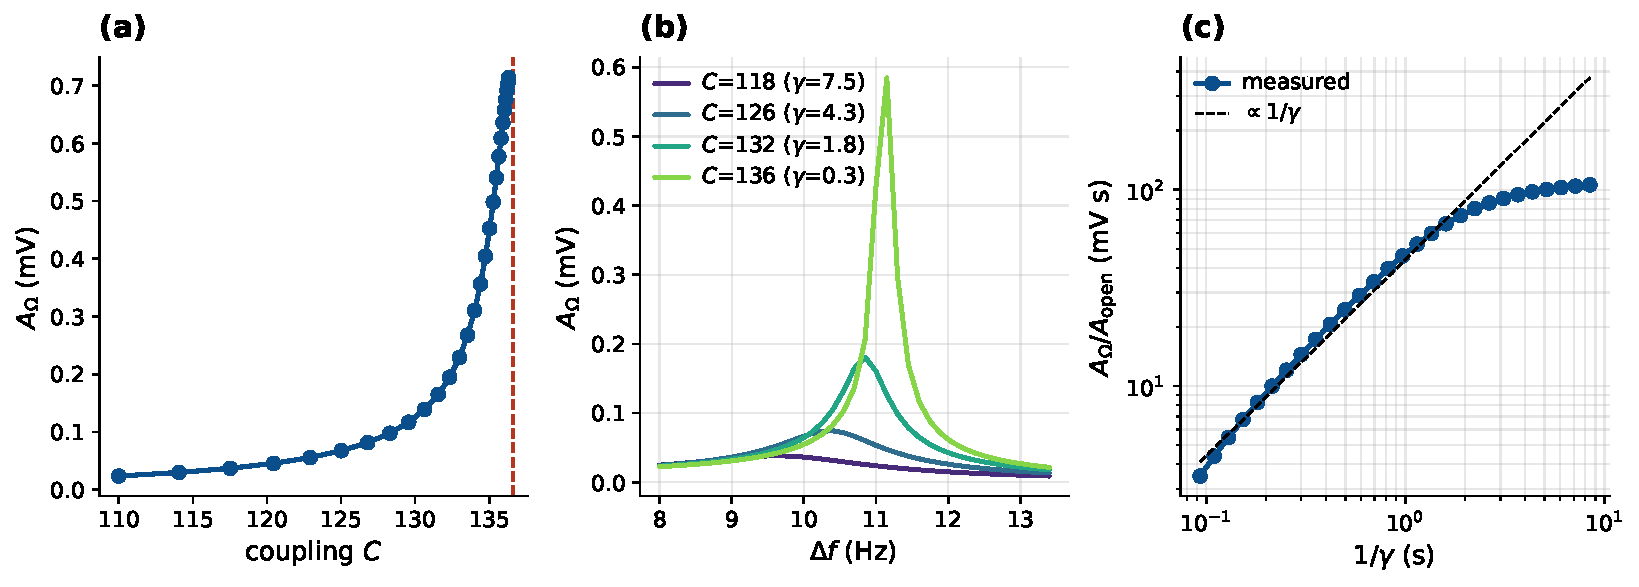
\includegraphics[width=\textwidth]{fig_jcurve.pdf}
\caption{\textbf{Coupling controls the amplification at fixed detection (Jansen--Rit).}
The operating point $v^*$ is pinned by co-solving $p(C)$, so $\Sig''(v^*)=-0.151$ and
$A_{\rm open}$ are held constant throughout. \emph{(a)} The demodulated $A_\Omega$ grows as the
coupling $C\,(=J)$ approaches the Hopf $C^*$ from the stable-focus side ($\gamma>0$). \emph{(b)} The envelope resonance
sharpens and grows as $C\!\to\!C^*$. \emph{(c)} The network gain
$A_\Omega/A_{\rm open}$ follows $1/\gamma$ (dashed) and saturates near the
bifurcation.}
\label{fig:jcurve}
\end{figure}

The next-generation theory gives the same result without pinning. In the NMM2 PING the
coupling $C$ is the \emph{literal} mean inter-neuron (QIF) synaptic weight $J$, and at this
carrier the generated source is operating-point independent to about $1\%$
(\S\ref{sec:dynamic}), so detection needs no pinning. Sweeping $J$ at fixed background drive
$\bar\eta$ toward the gamma Hopf $J^*$, the demodulated peak of $r_E$ grows as
$1/\gamma$ and saturates at criticality (Fig.~\ref{fig:nmm2_jcurve}): the heuristic JR
result, reproduced with the coupling \emph{and} the rectifier both derived rather than
assumed, and a direct counterpart of the coupling-controlled weak-field sensitivity of
QIF networks \cite{clusella2023}. The two columns \DIFdelbegin \DIFdel{realize one band-agnostic law }\DIFdelend \DIFaddbegin \DIFadd{exhibit the same gain scaling }\DIFaddend in
their two native \DIFdelbegin \DIFdel{bands---alpha }\DIFdelend \DIFaddbegin \DIFadd{bands, alpha }\DIFaddend (JR) and gamma (NMM2): the single-cell nonlinearity
detects the envelope (coarse-grained into $\Sig''$, or the exact $v^2$), while the
\DIFdelbegin \DIFdel{sharp, tunable gain is the network's---a resonant }\DIFdelend \DIFaddbegin \DIFadd{gain is a recurrent }\DIFaddend amplification set by proximity to the
Hopf and adjustable through the coupling.

\subsection{The resonance amplifies the envelope-locked modulation more than the mean rate}\label{sec:timing}
The demodulator feeds the network a constant term and a line at the beat $\Omega$
(Eq.~\eqref{eq:taylor}), and the transfer $G(\Omega)$ of Eq.~\eqref{eq:gain} treats them
differently: $G(\omega_0)\propto1/(2\gamma\omega_0)$ diverges as the Hopf is approached,
while $G(0)\propto1/\omega_0^2$ stays finite. Pinning $v^*$ to hold the local detector
curvature fixed, as in Fig.~\ref{fig:jcurve}, and driving the column toward the Hopf
through the coupling, we read both quantities from the same observable, the pyramidal
rate $r_P=\Sig(v+s)$ with the field in its argument. The beat-locked modulation of $r_P$ at
$\Delta f=f_0$ grows $13.5\times$ ($26$ to $346$~mHz), tracking $1/\gamma$ before
saturating near criticality; the shift of its mean grows too, $5.8\times$ ($-1.3$ to
$-7.7$~mHz), through rectification of the growing oscillation, but stays below $0.2\%$ of
the $3.9$~Hz baseline (Fig.~\ref{fig:timing}). Modulation exceeds mean shift by $19\times$
far from the Hopf and by $45$--$66\times$ near it. The network amplifies the
envelope-locked modulation far more than the mean rate, so a small mean-rate change is
the expected signature even where TI is acting, the mesoscopic counterpart of the
observation that TI alters spike timing more than firing rate in the primate brain
\cite{vieira2024}. Finite is not zero: the mean does move, and the comparison must use
commensurate measures, as here.

\subsection{Microscale confirmation: TI realigns spike timing in the QIF network}\label{sec:qif}
The mesoscale prediction has a direct microscale test, since NMM2 is the \emph{exact} mean
field of an all-to-all network of quadratic integrate-and-fire (QIF) neurons with
Lorentzian-distributed excitabilities
\cite{montbrio2015,ruffini2025rosetta,clusella2023}. Integrating that spiking network
($N=8000$ neurons per population, parameters identical to the PING mean field; Methods)
shows TI bunching spike \emph{times} into the beat cycle with a smaller change in the mean
rate, on both sides of the gamma Hopf (Fig.~\ref{fig:qif_raster}). Below the Hopf (forced)
the field-free network fires asynchronously at a flat rate; with TI on, spikes condense
into envelope-locked bands (Fig.~\ref{fig:qif_raster}a,b). Above the Hopf (oscillatory) the
free-running gamma is \emph{gated} by the TI \DIFdelbegin \DIFdel{beat---forced }\DIFdelend \DIFaddbegin \DIFadd{beat, a forced }\DIFaddend cross-frequency modulation
(phase--amplitude coupling, PAC), not frequency entrainment, since the $\approx$11~Hz detuning lies outside the
$1{:}1$ tongue: its bursts group into the $\Delta f=42$~Hz envelope while the intrinsic
$\sim$53~Hz gamma persists (Fig.~\ref{fig:qif_raster}c,d). Because the two rhythms coexist
in a nonlinear medium, the QIF nonlinearity mixes them into intermodulation sidebands in
the population rate---most prominently the direct $\Delta f$ line and the sum component near
$95$~Hz ($53\!+\!42$), with the difference tone near $11$~Hz (the detuning itself); this is
the spiking-network fingerprint of the same nonlinear frequency mixing that operates at the
macroscale, and it is the sideband signature of \emph{gating} rather than the frequency
pulling of entrainment. The spiking network reproduces
the exact NMM2 mean field's gamma spectrum (Fig.~\ref{fig:qif_timing}a). Across both
regimes the mean rate rises by $8$--$10\%$, while the $\Delta f$ modulation depth of the
population rate, $A_\Omega/\langle r_E\rangle$, rises from below $0.003$ to $0.29$ (forced)
and $0.23$ (gated) (Fig.~\ref{fig:qif_timing}c), measured over $44$ and $34$ whole beat
cycles after $800$~ms of settling (Methods). Timing modulation therefore exceeds the
relative mean-rate change by a factor of about three at the population level. Per neuron
the locking is weak: the pairwise phase consistency of single-neuron spike phases at
$\Delta f$ rises from its field-free control (median $-0.02$) to a median of
$0.003$--$0.005$, and the pooled vector strength from below $0.02$ to $0.12$--$0.13$. The
population's beat-locked component is built from many weakly biased cells, not from
strongly locked ones. This is the spiking-level counterpart of \S\ref{sec:timing} and a
qualitative analog of the in-vivo finding that TI alters spike timing more than firing
rate \cite{vieira2024}.

\begin{figure}[t!]
\centering
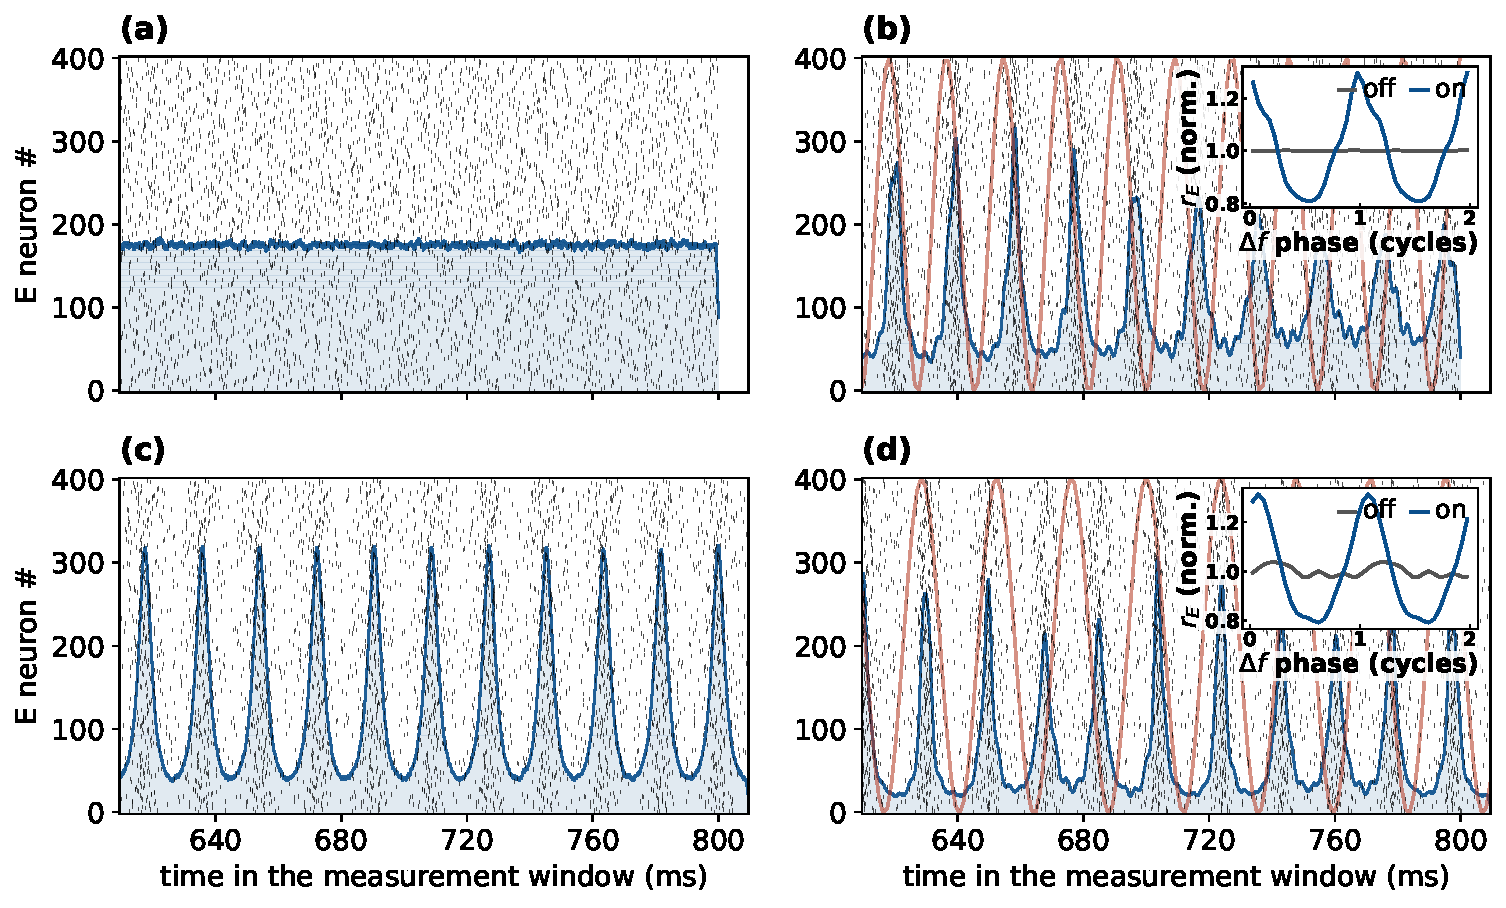
\includegraphics[width=\textwidth]{fig_qif_raster_twotone.pdf}
\caption{\textbf{QIF spiking network: TI bunches spikes into the beat cycle with a
smaller change in mean rate.} $N=8000$
excitatory and inhibitory quadratic integrate-and-fire neurons whose exact mean field is the
NMM2 PING circuit (Eq.~\eqref{eq:nmm2-ping}). The circuit's intrinsic rhythm is gamma
($\sim$53~Hz), so the beat is set in the gamma range (carrier $f_c=300$~Hz, genuine two
tones). Black ticks are $E$ spikes (400 of 8000), blue the population rate, red the TI
envelope; the bifurcation parameter is the common drive $\bar\eta$ (gamma Hopf at
$\approx 1.1$). \emph{(a,b)} Forced ($\bar\eta=0.85$), TI off then on at
$\Delta f=55$~Hz: asynchronous firing becomes envelope-locked bunching.
\emph{(c,d)} Oscillatory ($\bar\eta=1.5$), TI off then on with the beat detuned to
$42$~Hz: the free-running gamma persists but gains a $\Delta f$-locked component. Because
the $\approx$11~Hz detuning places the beat outside the $1{:}1$ tongue, this is forced
cross-frequency \emph{gating}, not frequency capture (contrast
Fig.~\ref{fig:entrain}); the detuning is what certifies the locked component as a driven
effect. The last $200$~ms of the $800$~ms measurement window are shown. \emph{Insets} in
\emph{(b,d)}: the population rate folded on the beat phase over the whole window ($44$ and
$34$ cycles), each normalized to its own mean (off gray, on blue); with that many cycles
the near-commensurate $53$~Hz gamma averages out of the $42$~Hz fold in \emph{(d)}. Both
are flat with TI off.}
\label{fig:qif_raster}
\end{figure}

\subsection{Falsifiable predictions and tests}\label{sec:predictions}
The mechanism makes four predictions, each with an experimental handle.
\begin{enumerate}[leftmargin=*]
\item \textbf{Carrier \DIFdelbegin \DIFdel{independence at fixed polarization}\DIFdelend \DIFaddbegin \DIFadd{dependence separates access from mixing}\DIFaddend .} \DIFdelbegin \DIFdel{Once the post-coupling
polarization $\varepsilon=\lambda_f E_0$ is matched}\DIFdelend \DIFaddbegin \DIFadd{In the static limit
and in the fast-carrier QIF asymptote}\DIFaddend , the leading \DIFdelbegin \DIFdel{quadratic beat component
no longer depends on }\DIFdelend \DIFaddbegin \DIFadd{beat is independent of }\DIFaddend $f_c$ \DIFaddbegin \DIFadd{at
fixed local polarization}\DIFaddend , provided the carrier \DIFdelbegin \DIFdel{lies outside the responsive bands of both
detector and network ; frequency dependence
reappears through the effective coupling
$\lambda_f=\lambda_0|H_c(f_c)|$, or when a fast cellular or network stage is itself resonant
(\S\ref{sec:lanmm-results}). The \emph{applied}-field threshold still rises with $f_c$
through the membrane roll-off }\DIFdelend \DIFaddbegin \DIFadd{does not excite another network mode.
At fixed applied field, access restores frequency dependence
}\DIFaddend (Eq.~\eqref{eq:khz})\DIFdelbegin \DIFdel{---as single-neuron accounts also
predict \cite{opancar2025,mirzakhalili2020}.
\emph{Test:} hold the in-zone
polarization fixed (raising $E_0$ to compensate the measured $\lambda_f$) while
sweeping $f_c$; the network signature is a flat envelope response. At fixed applied
field the same sweep reads the entry point: the roll-off should sit in the kHz range (AIS
access, Na$_{\rm v}$ gating), not at the $\sim$10~Hz somatic corner (\S\ref{sec:khz}). Existing
AM-versus-tACS comparisons match the extracellular modulation rather than $\varepsilon$
\cite{vieira2024}, so this is the correction they lack}\DIFdelend \DIFaddbegin \DIFadd{; detector dynamics can add it near the crossover.
\emph{Test:} measure or estimate local polarization during a carrier sweep and
compare the response before and after correcting for access}\DIFaddend . \DIFaddbegin \DIFadd{The remaining
frequency dependence constrains the mixing mechanism. Its cutoff is to be
measured, not assigned to a particular compartment in advance.
}\DIFaddend \item \textbf{State- and carrier-dependent response.} The generated beat depends on
the operating point through the detector coefficient, and the two modeled detectors
disagree on how: the memoryless sigmoid follows $\Sig''(v^*)$ and reverses sign across the
inflection, where PEIX (Eq.~\eqref{eq:peix}) peaks; the dynamic mean field at a fast
carrier follows $F'$ and the network susceptibility, without a sign rule
(\S\ref{sec:dynamic}). \emph{Test:} \DIFdelbegin \DIFdel{shift $v^*$ with tonic drive , neuromodulation, or task
state at a fixed beat, and sweep the carrier at a fixed beat }\DIFdelend \DIFaddbegin \DIFadd{vary tonic drive and carrier frequency while
measuring both amplitude and phase of the beat response. Compare these with the
predicted mixing coefficient after accounting for changes in network susceptibility;
a response-amplitude change alone does not isolate the detector}\DIFaddend .
\DIFdelbegin \DIFdel{A sign reversal across the
operating point would select the memoryless description, a monotonic change the dynamic
one.
}\DIFdelend \item \textbf{Transduction class.} A weak smooth nonlinearity transduces $A^2$ and an
envelope follower transduces $A$ (\S\ref{sec:transduction}), and the two are separable at a
single matched target. The former gives $Y_\Omega\propto\varepsilon^2$ with a second-harmonic
ratio vanishing as $\varepsilon\!\to\!0$; the latter gives $Y_\Omega\propto\varepsilon$ with
the ratio pinned at $1/5$. \emph{Test:} sweep field amplitude off resonance (so that both
lines sit on the flat part of $G$) and read the log--log slope together with
$Y_{2\Omega}/Y_\Omega$; on resonance the network suppresses the second harmonic by
$\sim 3\mathcal{Q}$ and the test must be corrected by an independently measured
$G(2\Omega)/G(\Omega)$.

\item \textbf{Frequency selectivity and state-dependence.} The response is largest
when $\Delta f$ matches a region's resonant rhythm and is amplified as $1/\gamma$ near
a bifurcation\DIFdelbegin \DIFdel{, so manipulations that move the operating point or the distance to the
Hopf---psychedelics, PV-interneuron dysfunction, attention, arousal---should scale,
and can abolish or sign-reverse, TI efficacy }\DIFdelend \DIFaddbegin \DIFadd{. Changes in operating state can therefore alter both the generated
drive and the recurrent gain }\DIFaddend \cite{ruffini2025cfc}. \emph{Test:}
sweep $\Delta f$ through a region's intrinsic band across brain states and track the
resonant peak and its width.
\end{enumerate}

Table~\ref{tab:predictions} \DIFdelbegin \DIFdel{confronts these predictions---together with two corollaries
the mechanism already shares with published observations---against }\DIFdelend \DIFaddbegin \DIFadd{compares the predictions and related model consequences
with }\DIFaddend existing evidence.
Two are qualitatively consistent with published observations: TI alters spike timing
more than firing rate in vivo \cite{vieira2024} (our $G(\omega_0)\!\gg\!G(0)$ asymmetry,
\S\ref{sec:timing}--\ref{sec:qif}), and most pyramidal TI responses vanish when synaptic
transmission is blocked \cite{caldas2024} (a network read-out, which tests network
involvement rather than excluding a surviving cellular detector). A
quantitative reanalysis of these datasets against the model is a natural next step, and
\S\ref{sec:discussion} specifies the amplitude-exponent fit it would require.

\begin{table}[h]
\centering\small
\renewcommand{\arraystretch}{1.25}
\DIFdelbeginFL %DIFDELCMD < \begin{tabular}{@{}p{0.27\textwidth} p{0.35\textwidth} p{0.30\textwidth}@{}}
%DIFDELCMD < %%%
\DIFdelendFL \DIFaddbeginFL \begin{tabular}{@{}>{\raggedright\arraybackslash}p{0.27\textwidth} >{\raggedright\arraybackslash}p{0.35\textwidth} >{\raggedright\arraybackslash}p{0.30\textwidth}@{}}
\DIFaddendFL \toprule
\textbf{Prediction (model basis)} & \textbf{Existing evidence} & \textbf{Sharp test} \\
\midrule
Transduction class: $Y_\Omega\propto\varepsilon^2$ and vanishing $Y_{2\Omega}/Y_\Omega$
(square law) vs.\ $\propto\varepsilon$ and $1/5$ (envelope following) & --- (untested;
existing comparisons match extracellular field, not $\varepsilon$) & Amplitude sweep off
resonance; transfer-corrected harmonic ratio \\
Timing-dominated response: the envelope-locked modulation of the rate grows toward
the Hopf faster than its mean ($G(\omega_0)\!\gg\!G(0)$) & \emph{Qualitatively
consistent}: TI alters spike timing more than firing rate, primate \cite{vieira2024} &
Lock-in of spike timing at $\Delta f$ vs.\ the mean-rate change, in the same effect
measure \\
Network read-out (population nonlinearity + synaptic recurrence) &
\emph{Qualitatively consistent}: most pyramidal TI responses vanish under synaptic block
\cite{caldas2024} & Synaptic block should \DIFdelbeginFL \DIFdelFL{abolish the demodulated response }\DIFdelendFL \DIFaddbeginFL \DIFaddFL{reduce recurrent amplification; cellular
mixing may persist }\DIFaddendFL \\
Carrier independence at fixed polarization (no $\omega_c$ in $A_\Omega$) & TI thresholds
inherit the carrier's $f_c$-dependence \cite{opancar2025,peripheral2023}; bare kHz weakly
effective \cite{esmaeilpour2020} & Fix in-zone polarization, sweep $f_c\!\to$ flat envelope
response \DIFdelbeginFL \DIFdelFL{; at fixed field, a kHz-range (not 10~Hz) roll-off }\DIFdelendFL \DIFaddbeginFL \DIFaddFL{in the stated limits; fit access and residual detector dependence }\DIFaddendFL \\
State- and carrier-dependent response (the detector coefficient is model-dependent) &
Cell-type-specific TI responses (PV vs.\ pyramidal) \cite{caldas2024} & Shift $v^*$ by
state at fixed beat; sweep $f_c$ at fixed beat \\
Frequency selectivity, sharpened $\sim1/\gamma$ near criticality & \DIFdelbeginFL \DIFdelFL{--- (a sharp new
prediction; largely untested) }\DIFdelendFL \DIFaddbeginFL \DIFaddFL{Quantitative
gain--bandwidth relation not tested here in biological data }\DIFaddendFL & Sweep $\Delta f$ through a region's band across brain
states \\
\bottomrule
\end{tabular}
\caption{The mechanism's predictions confronted with existing in-vivo / in-vitro evidence.
Entries cite documented qualitative findings; quantitative reanalysis is left to future
work.}\label{tab:predictions}
\end{table}

\section{Discussion}\label{sec:discussion}
\DIFdelbegin \DIFdel{\textbf{The models show how neural populations can act as tuned receivers of TI
inputs.} Nonlinear mixing generates a component at the
difference frequency , and recurrent
dynamics selectively amplify it near a network resonance. Generation and amplification are
distinct contributions: a large network response does not, by itself, imply efficient
detection. This complements rather than competes with the single-neuron }\DIFdelend \DIFaddbegin \DIFadd{The population models separate the generation of a difference-frequency drive from
its recurrent amplification. Cellular mixing can supply that drive, while the
network determines its frequency selectivity and gain. This interpretation connects
the }\DIFaddend ion-channel \DIFdelbegin \DIFdel{account \cite{mirzakhalili2020}: both are rectify-then-filter demodulation, ours is
agnostic about which fast cellular nonlinearity supplies the mixing, and it inherits the
brain's own resonances, so a region's tuning is set by its intrinsic dynamics as a radio
is tuned by its tank}\DIFdelend \DIFaddbegin \DIFadd{mechanism \cite{mirzakhalili2020,luff2024mixer} to the network
dependence seen in slices and simulations \cite{caldas2024,karimi2024,soroushi2025}.
It does not require cellular mixing and circuit amplification to be competing
explanations}\DIFaddend .

\DIFdelbegin \DIFdel{\textbf{The detector's dynamics matter.} The }\DIFdelend \DIFaddbegin \DIFadd{The distinction between a }\DIFaddend static sigmoid and \DIFdelbegin \DIFdel{the dynamic }\DIFdelend \DIFaddbegin \DIFadd{a dynamic population functional is a
time-scale distinction. In the slow-synapse limit, the exact }\DIFaddend QIF mean field \DIFdelbegin \DIFdel{both support quadratic mixing in the weak-response regime, but their mixing coefficients
and operating-point dependence differ (\S\ref{sec:dynamic}).
A steady-state firing-rate
curve therefore does not, on its own, determine the response to a fast carrier. The common
mechanism is nonlinear mixing followed by network tuning, not a universal
sigmoid-curvature law. The
single cell need only supply a fast nonlinearity that samples
the carrier; in the exact mean field that is the spike-generating quadratic acting on a voltage excursion of order $a/\omega$.
A population transferfunctional calibrated to the relevant cellular dynamics could
incorporate ion-channel mixing. A static firing-rate sigmoid specifies only the
steady-state relation; its curvature }\DIFdelend \DIFaddbegin \DIFadd{reduces
to the nonlinear curve in Eq.~\eqref{eq:Fmpr} while synapses retain their dynamics.
If relaxation is also fast relative to the carrier, the curve's curvature gives
the leading beat. Otherwise, the dynamic mixing calculation is required. The
curve's slope has a separate role: it converts a slow input into a rate change and
sets the local gain entering recurrent feedback. This reduction explains what
can be included in a population transfer, but }\DIFaddend does not establish that \DIFdelbegin \DIFdel{dynamic functional or its
carrier-frequency dependence.}\DIFdelend \DIFaddbegin \DIFadd{a particular
QIF parameterization reproduces the channel mechanisms measured by Luff et al.\
\cite{luff2024mixer}. That identification requires matching the relevant dynamical
response, not only a steady-state firing-rate curve.
}\DIFaddend

\DIFdelbegin \DIFdel{\textbf{Where the carrier-sampling nonlinearity may live.} The literature points to three
non-exclusive loci. (i)~\emph{Axonal Na$^+$ channels} at nodes }\DIFdelend \DIFaddbegin \DIFadd{Fast access has several possible anatomical and electrical origins. Nodes }\DIFaddend and the
AIS \DIFdelbegin \DIFdel{, where fast
}\DIFdelend \DIFaddbegin \DIFadd{contain }\DIFaddend voltage-gated \DIFdelbegin \DIFdel{Na$^+$ rectifies because activation outpaces inactivation
\cite{mirzakhalili2020,wang2023}and inactivation-mediated block passes the slow envelope
while removing the carrier \cite{opancar2025}. (ii)~\emph{Presynaptic terminals}, which
polarize $\sim$2--10$\times$ more }\DIFdelend \DIFaddbegin \DIFadd{channels capable of nonlinear rectification
\cite{mirzakhalili2020,wang2023}. Presynaptic terminals can polarize more strongly
}\DIFaddend than somata \cite{rahman2013,aberra2023,chakraborty2018}\DIFdelbegin \DIFdel{and convert depolarization into release through a steeply nonlinear Ca$^{2+}$ relation.
Sensitivity is not speed, however}\DIFdelend \DIFaddbegin \DIFadd{, but small size alone does
not imply fast charging}\DIFaddend : for an isopotential \DIFdelbegin \DIFdel{compartment $\tau_m=R_mC_m$ with
both quantities per unit area, so the time constant does not shrink with size---a small
bouton has small capacitance and correspondingly large input resistance . A terminal
therefore tracks a kHz carrier no better than a soma, and the short axonal time constants
come from high-conductance nodal membrane rather than from small size. Terminals are the
\emph{sensitive} locus, not the fast one}\DIFdelend \DIFaddbegin \DIFadd{membrane, the product of specific
resistance and capacitance is independent of area. Conductance, geometry}\DIFaddend , and the
\DIFdelbegin \DIFdel{carrier sampling is supplied
by~(i). (iii)~\emph{Threshold spiking}, where a weak bias near threshold is rectified
through stochastic resonance \cite{liu2018,reato2010}. Each is a candidate; the simulations impose an access filter and a nonlinearity, they do not identify the
compartment}\DIFdelend \DIFaddbegin \DIFadd{mode of stimulation determine the response}\DIFaddend .

\DIFdelbegin \DIFdel{The periaxonal space provides another candidate access route. }\DIFdelend Cohen et al.\ \cite{cohen2020periaxonal} \DIFdelbegin \DIFdel{combined recordings, electron microscopy, and cable modeling
to establish a conducting space between the axon membrane and myelin, }\DIFdelend \DIFaddbegin \DIFadd{established a conducting periaxonal space
}\DIFaddend approximately $12$~nm wide\DIFdelbegin \DIFdel{and incompletely }\DIFdelend \DIFaddbegin \DIFadd{, partly }\DIFaddend sealed at the paranodes\DIFdelbegin \DIFdel{. Their double-cable model separates
the potentials across the myelin sheath and the underlying axon membrane. This
architecture motivates computing the transfer from an applied extracellular kHz field
to the local voltage at a candidate mixer. The saltatory-conduction measurements do not
determine that transfer. }\DIFdelend \DIFaddbegin \DIFadd{, and modeled the distinct
potentials across myelin and the axonal membrane. Their methods report a minimum
fitted axonal decay time near $1$~ms; this is not a measured TI access time.
Luff et al.'s PWM-TI model likewise includes a $1$~ms passive response within a
$1$--$100$~ms parameter sweep \cite{luff2024}. Separately, Semenov et al.\
\cite{semenov2025} measured field-induced membrane charging near $0.7~\mu$s in
isolated neurons under strong, microsecond field pulses. This is a different
response mode from intracellular current charging or periaxonal conduction.
Together these studies motivate examining a shorter effective access time, while
leaving its value and field coupling preparation-dependent. }\DIFaddend A $10$--$100$-fold
\DIFdelbegin \DIFdel{shorter effective carrier-access time scale
}\DIFdelend \DIFaddbegin \DIFadd{reduction }\DIFaddend in a QIF \DIFdelbegin \DIFdel{reduction remains a modeling hypothesisto test against this geometry. Changing
the QIF membrane time scale also requires recomputing its operating point and resonance}\DIFdelend \DIFaddbegin \DIFadd{membrane time is therefore a sensitivity hypothesis. Its
population-level consequence can be studied through the existing slow-synapse
limit}\DIFaddend , with each physical \DIFdelbegin \DIFdel{filtering process represented once.
}\DIFdelend \DIFaddbegin \DIFadd{filter included once; a new periaxonal circuit is not
needed for that limiting argument.
}\DIFaddend

\DIFdelbegin \DIFdel{\textbf{The conventional TI dose map is an assumption about physiology, not a consequence
of field physics.} The envelope is a mathematical property of a high-frequency waveform. It
is not
itself a low-frequency field, and nothing in Maxwell's equations delivers it to a
neuron; biology must construct it.
Targeting work since \cite{grossman2017} takes the
}\DIFdelend \DIFaddbegin \DIFadd{A spatial TI dose map depends on this physiology. The usual }\DIFaddend envelope-modulation
\DIFdelbegin \DIFdel{amplitude $\mathcal{M}[A]=2\min(\varepsilon_1,\varepsilon_2)$ as the
spatial dose, which assumes $R(\mathbf{x})=\Phi(\mathcal{M}[A])$ for monotonic $\Phi$---that
the response depends on }\DIFdelend \DIFaddbegin \DIFadd{measure $\mathcal M[A]=2\min(\varepsilon_1,\varepsilon_2)$ assumes that neural
response is determined by }\DIFaddend the envelope excursion\DIFdelbegin \DIFdel{\emph{alone}, and not separately on the carrier baseline,
the operating point or the orientation. That assumption is substantive, and a weak smooth nonlinearity cannot satisfy it: }\DIFdelend \DIFaddbegin \DIFadd{. In the local square-law regime,
the beat instead depends on $\varepsilon_1\varepsilon_2$, and }\DIFaddend the carrier average
\DIFdelbegin \DIFdel{Eq.~\eqref{eq:cycavg} is invariant under $A\to-A$, so its expansion contains only even
powers and no }\DIFdelend \DIFaddbegin \DIFadd{also contains a DC }\DIFaddend term proportional to \DIFdelbegin \DIFdel{$A$ exists.
Square-law transduction is therefore the
generic perturbative answer and envelope following is the special case needing
justification, since recovering $A$ requires rectification (\S\ref{sec:transduction}) and
any \emph{smoothed} threshold reverts to $A^2$ as the field weakens.
}\DIFdelend \DIFaddbegin \DIFadd{$\varepsilon_1^2+\varepsilon_2^2$.
Orientation, access, operating point, and network susceptibility further shape
the response. For a smooth memoryless transfer, carrier averaging is even in the
envelope amplitude, giving quadratic transduction when the second-order coefficient
is nonzero. Dynamic nonlinearities can also mix at second order, with
frequency-dependent coefficients. A sharp rectifier can instead approximate
envelope following over a finite amplitude range; smoothing or heterogeneity
can restore quadratic behavior at smaller inputs. The amplitude and harmonic
tests in \S\ref{sec:transduction} distinguish these regimes.
}\DIFaddend

\DIFdelbegin \DIFdel{Different field strengths and operating states may recruit different nonlinear
mechanisms; the present analysis addresses the weak-response regime. Near threshold a
sharp channel or spike nonlinearity may act as a rectifier; well below it, the leading
responseof any smooth nonlinearity, memoryless or dynamic, is quadratic mixing, filtered
and amplified by the network as described here. Which of the two operates at human field
strengths is an empirical question that present evidence does not settle. Primate
recordings at human-comparable fields find an AM waveform less effective than matched-depth
tACS, but do not estimate the difference closely enough to select a transduction law
\cite{vieira2024}, and peripheral-nerve work argues that some TI responses reflect carrier
integration rather than envelope extraction \cite{peripheral2023}. Two 2025 studies sharpen
that point at suprathreshold intensities: in peripheral nerves the strength--frequency
curves of TI, amplitude-modulated }\DIFdelend \DIFaddbegin \DIFadd{Stimulation intensity can also change the mechanism. At high intensities, TI }\DIFaddend and
unmodulated kHz \DIFdelbegin \DIFdel{waveforms overlap
\cite{opancar2025}, and in isolated hippocampal neurons pure $2$ and $20$~kHz fields excite
at high intensity while modulation
patterns the firing without }\DIFdelend \DIFaddbegin \DIFadd{fields can have similar excitation thresholds, with modulation
patterning firing rather than }\DIFaddend lowering the threshold
\DIFdelbegin \DIFdel{\cite{semenov2025}. At those intensities the carrier itself stimulates. The weak-field
mixing route analyzed here is a candidate for the subthreshold, modulatory regime of the
primate recordings and of the recent patient studies of hippocampal TI \cite{vieira2024,missey2026}. What settles it is not whether TI works but which quantity
it transduces, and \S\ref{sec:transduction} gives the measurement. }\DIFdelend \DIFaddbegin \DIFadd{\cite{opancar2025,semenov2025}; some peripheral responses do not require envelope
extraction \cite{peripheral2023}. The weak-input calculation here concerns
subthreshold mixing and its amplification. It provides a candidate mechanism for
modulatory responses, not a common explanation for every TI preparation
\cite{vieira2024,missey2026}.
}\DIFaddend

\DIFdelbegin \DIFdel{\textbf{The amplifier is not specific to TI.} A tACS field oscillates in the envelope band
directly and needs no demodulation, but it drives the same near-Hopf resonator. Sweeping
the coupling toward the alpha Hopf at \emph{pinned} operating point , a direct $\Delta f$
drive reproduces }\DIFdelend \DIFaddbegin \DIFadd{The recurrent amplifier is shared with direct low-frequency stimulation. In our
coupling sweep, holding the JR operating point fixed holds the local curvature
fixed while the network gain changes. A direct in-band drive shows }\DIFaddend the same
$1/\gamma$ growth and resonance sharpening \DIFdelbegin \DIFdel{as the demodulated TI
drive, linear in the field rather than square-law }\DIFdelend (Fig.~\ref{fig:tacs})\DIFdelbegin \DIFdel{. Coupling-controlled gain is known: the dynamical transfer function of an E--I network is
known to become resonant near a Hopf bifurcation, with a peak that \emph{diverges} on the bifurcation line as connectivity is varied \cite{ledoux2011}, and increased
self-connectivity is known to enhance weak-field resonant sensitivity in the exact mean
field \cite{clusella2023}. What the pinned sweep adds is the separation of amplification
from \emph{detection}. Holding the local detector curvature $\Sig''(v^*)$ constant while
the network transfer changes isolates the network gain, and shows that the same amplifier
acts on a drive the population has itself generated. TI then differs from tACS by a
generating front end that converts a kHz carrier pair into an effective in-band drive;
downstream, both share the criticality- and coupling-controlled amplifier, so, matched for
effective in-band drive, read through the same observable and near the same state, they
should entrain alike. The cancellation is conditional on those matches.
}%DIFDELCMD <

%DIFDELCMD < %%%
\DIFdel{\textbf{Amplification is critical slowing, of a mean-field kind.} Gain $\propto1/\gamma$
as the damping vanishes at the Hopf is the diverging susceptibility of a system
approaching a bifurcation. In the exact next-generation mean field the reduction from the
spiking population is exact in the thermodynamic limit and $(r,v)$ are order parameters
\cite{ott2008,montbrio2015}, so the Hopfis a macroscopic transition; because the
reduction assumes all-to-all coupling the critical point is mean-field, with }\DIFdelend \DIFaddbegin \DIFadd{, consistent with
the known resonant susceptibility of recurrent excitatory--inhibitory networks
\cite{ledoux2011,clusella2023}. Near the Hopf, this is }\DIFaddend temporal critical slowing
\DIFdelbegin \DIFdel{but no }\DIFdelend \DIFaddbegin \DIFadd{in a mean-field model, not evidence of a }\DIFaddend diverging spatial correlation length.
\DIFdelbegin \DIFdel{The coupling sweep moves
the model toward the bifurcation; the stimulus probes its response.
}%DIFDELCMD <

%DIFDELCMD < %%%
\DIFdel{\textbf{Prior work already places the operative nonlinearity in the network.} Recurrent
excitation, with short-term synaptic depression, accounts for tACS entrainment in a
large-scale spiking model and yields an Arnold tongue over stimulation amplitude and
frequency \cite{ali2013}; the dynamical transfer function of an E--I network, in both rate
and spiking form, is resonant near a Hopf bifurcation with a peak that diverges on the
bifurcation line as the connectivity is swept \cite{ledoux2011}; an amplitude-modulated
high-frequency drive phase-locks a cortical model to its envelope through the same target
engagement as low-frequency tACS \cite{negahbani2018}; and comparing neuron models directly,
integrate-and-fire membranes fail to reproduce observed TI behavior while
Hodgkin--Huxley ones succeed \cite{plovie2025}. The general case for stimulation as
interaction with ongoing dynamics has been made explicitly \cite{krause2023}. What we add
is the separation of the generated source from the network response , the comparison of a
memoryless and a dynamic detector, }\DIFdelend \DIFaddbegin \DIFadd{Related models already reproduce tACS entrainment }\DIFaddend and \DIFdelbegin \DIFdel{, downstream of both, that the
transduced quantity
in the weak-response regime is $A^2$ rather than $A$, a distinction the cited network
studies do not draw. }\DIFdelend \DIFaddbegin \DIFadd{AM-driven phase locking
\cite{ali2013,negahbani2018,krause2023}. The separation here is between the drive
generated by mixing and the response to that drive. When TI and tACS are matched
for effective in-band input, observable, and operating state, they share the
amplifier. Resonance alone therefore gives TI no efficiency advantage.
}\DIFaddend

\DIFdelbegin \DIFdel{\textbf{Estimated response magnitude and comparison with tACS.} Two obstacles separate a
transcranial field from a response at $\Delta f$, and they need different answers.
The first is that weak fields barely move a membrane: measured coupling is
}\DIFdelend \DIFaddbegin \DIFadd{Absolute response estimates remain sensitive to access and transduction.
Measured static field-to-voltage couplings are }\DIFaddend $0.12$--$0.21$~mV per V/m in
hippocampus \cite{bikson2004,deans2007} and \DIFdelbegin \DIFdel{up to
$\sim 0.5$}\DIFdelend \DIFaddbegin \DIFadd{reach about $0.5$}\DIFaddend ~mV per V/m \DIFdelbegin \DIFdel{for }\DIFdelend \DIFaddbegin \DIFadd{in }\DIFaddend cortical
L5/6 pyramidal cells \cite{radman2009}\DIFdelbegin \DIFdel{, human cortex
sees about }\DIFdelend \DIFaddbegin \DIFadd{; human cortical fields near }\DIFaddend $0.8$~V/m \DIFdelbegin \DIFdel{at 2}\DIFdelend \DIFaddbegin \DIFadd{have
been reported at $2$}\DIFaddend ~mA \cite{huang2017,huang2017corr}\DIFdelbegin \DIFdel{, and most applied current is shunted through scalp and skull \cite{voroslakos2018}. The field shifts a soma by a few
tenths of a millivolt against the $\sim 23$~mV separating rest from threshold
\cite{koga2010}. This is
as true of tACS as of TI. The second belongs to TI alone: its field carries no
power at $\Delta f$, so the response there must be generated by a nonlinearity. Resonance
addresses the first, a population near its own bifurcation responding to a weak push far
more strongly than an isolated cell, but not the second, because it amplifies TI and tACS
alike and cancels when the two are compared under the matching conditions above}\DIFdelend \DIFaddbegin \DIFadd{. These static couplings do
not fix the coupling at kHz. For equal TI carrier polarizations $\varepsilon$,
the JR beat drive is $\Sig''\varepsilon^2/2$, whereas a direct drive of the same
peak polarization gives $2\Sig'\varepsilon$. Their leading amplitude ratio is
$\eta_{\rm det}\simeq|\Sig''|\varepsilon/(4\Sig')$: the relative efficiency decreases
with input amplitude in this perturbative regime. A larger recurrent gain
amplifies both drives}\DIFaddend .

\DIFdelbegin \DIFdel{The resonance contributes a factor of order ten. With $\tau=1/\gamma$ the reverberation time , the
gain at resonance relative to the same circuit's response to a steady input is
$\mathcal{Q}=\pi f_0\tau$. Cortical population activity relaxes }\DIFdelend \DIFaddbegin \DIFadd{For scale, a reverberation time $\tau_{\rm rev}=1/\gamma$ gives a near-Hopf
quality factor $\mathcal Q\simeq\pi f_0\tau_{\rm rev}$ and power bandwidth
approximately $1/(\pi\tau_{\rm rev})$. Population relaxation }\DIFaddend over a few hundred
milliseconds \cite{wilting2018} \DIFdelbegin \DIFdel{, giving $\mathcal{Q}$ of order $10$ at
$f_0=10$~Hz---an
order of magnitude, not a value, since that timescale is wideband rather than
alpha-specific. Gain also costs bandwidth : the resonance is $1/(\pi\tau)$ wide in power (full width at
half maximum), about }\DIFdelend \DIFaddbegin \DIFadd{would give a quality factor of order ten at
$10$~Hz and a bandwidth of order }\DIFaddend $1$~Hz\DIFdelbegin \DIFdel{, so a $\Delta f$ fixed at a group-mean alpha may sit outside
it; whether an individual's alpha drifts that far within a session is not settled by this
estimate. At equal field strength TI is far weaker than tACS for the memoryless detector at
matched peak polarization. With per-carrier polarizations $\varepsilon_{1,2}$ the
demodulated drive is
$\half\Sig''\varepsilon_1\varepsilon_2$ against $2\Sig'\varepsilon$ for tACS at the same
peak polarization, a ratio $\eta_{\rm det}=\Sig''\varepsilon/4\Sig'$ proportional to
$\varepsilon$:
a square-law detector gets \emph{less} efficient as the signal weakens.
Formally $\eta_{\rm det}$ reaches unity near $\varepsilon\approx7$~mV, but that is the order of the
distance to threshold and lies outside the expansion's validity, so parity is not reachable
by this route rather than merely expensive. At $1$~V/m with a $1$~kHz carrier---now
comparing at matched \emph{applied} field, so the carrier's membrane attenuation enters
twice while the in-band tACS drive is unfiltered---TI comes out $\sim 300\times$ weaker
than tACS if the carrier reaches a fast nodal compartment, and $\sim 10^6\times$ weaker if
it reaches only the soma. }\DIFdelend \DIFaddbegin \DIFadd{. This is an order-of-magnitude comparison:
the measured relaxation is not specific to the alpha mode. Narrow amplification
also makes detuning consequential.
}\DIFaddend

\DIFdelbegin \DIFdel{The one in-regime measurement sits well above this estimate. }\DIFdelend \DIFaddbegin \DIFadd{Primate measurements illustrate both the relevance and the limits of an efficiency
comparison. }\DIFaddend Vieira et al.\ \DIFdelbegin \DIFdel{worked at
}\DIFdelend \DIFaddbegin \DIFadd{\cite{vieira2024} used }\DIFaddend modulation depths of
$0.5$--$0.62$~V/m \DIFdelbegin \DIFdel{, chosen deliberately to match human studies rather
than the $60$--$383$~V/m of the rodent literature, and report TI }\DIFdelend \DIFaddbegin \DIFadd{and reported TI effects }\DIFaddend at $0.34$ times \DIFdelbegin \DIFdel{the
strength }\DIFdelend \DIFaddbegin \DIFadd{those }\DIFaddend of conventional
tACS (\DIFdelbegin \DIFdel{$95\%$ CI }\DIFdelend \DIFaddbegin \DIFadd{95\% confidence interval }\DIFaddend $0.04$--$0.65$)\DIFdelbegin \DIFdel{, or $\sim 12\%$ per unit current
under their stated assumption that effects are roughly proportional to applied current
\cite{vieira2024}. That normalization is not neutral here, since a square-law drive scales
as $I^2$ while tACS scales as $I$; the per-current figure is therefore
transduction-class-dependent and we do not use it. Their AM-versus-tACS comparison
is the
most direct available. Having measured that transcranial current is shunted increasingly
with frequency, they compensate for it and deliver conventional tACS and an AM waveform
through the same electrodes, with the }\DIFdelend \DIFaddbegin \DIFadd{. Their within-electrode AM comparison
compensated for frequency-dependent current shunting and matched extracellular
}\DIFaddend modulation depth near the recorded cells\DIFdelbegin \DIFdel{calibrated
to $1.14$--$1.17$ times the tACS amplitude. Against a baseline PLV of $0.043$, tACS raises
the median to $0.20$ ($95\%$ CI $0.043$--$0.64$) and AM-tACS to $0.10$
($0.023$--$0.38$), a paired difference significant at $p=0.01$}\DIFdelend . \DIFdelbegin %DIFDELCMD <

%DIFDELCMD < %%%
\DIFdel{Taking their fields with a favorable cortical coupling ($\sim 0.5$~mV per V/m) through a
fast element at $2$~kHz gives $\varepsilon\!\approx\!0.1$~mV and hence
$\eta\!\approx\!0.8\%$, far below the
ordering they report; a somatic route is worse by two
further orders. Three limits keep this from being a quantitative test. The comparison rests
on }\DIFdelend \DIFaddbegin \DIFadd{A favorable fast-access estimate with
$\varepsilon\approx0.1$~mV gives only about $0.8\%$ for the JR detector, below the
reported ratio. This discrepancy is not a calibrated rejection of that detector:
the comparison involved }\DIFaddend twenty neurons, \DIFdelbegin \DIFdel{of which ten responded }\DIFdelend \DIFaddbegin \DIFadd{with ten responding }\DIFaddend to at least one
modality and seven to both\DIFdelbegin \DIFdel{, so
the sample is selected for responsiveness and the reported intervals are correspondingly
broad. PLVis a downstream statistic that }\DIFdelend \DIFaddbegin \DIFadd{; phase-locking value (PLV) }\DIFaddend depends on baseline locking
\DIFdelbegin \DIFdel{, network
susceptibility and state as well as on the generated drive, and in their full dataset
baseline PLV predicts the sign as well as the size of the change. And the quantity matched was the extracellular modulation, not }\DIFdelend \DIFaddbegin \DIFadd{and network state; and }\DIFaddend the \DIFdelbegin \DIFdel{post-coupling polarization $\varepsilon=\lambda_f E$ of \S\ref{sec:coupling} at whichever compartment supplies the nonlinearity, so the ratio reports the whole end-to-end path from applied field through
frequency-dependent access, transduction, network dynamics and spike-phase statistics. It
does not isolate the transducer. What the experiment establishes is that a high-frequency
AM waveform drives phase locking less effectively than a }\DIFdelend \DIFaddbegin \DIFadd{matched extracellular fields do not ensure matched
polarization at the cellular mixer. An unspecified nonlinear relation between
generated drive and PLV also prevents identification of the input-amplitude
exponent. The data establish a weaker AM effect than the }\DIFaddend matched-depth
low-frequency \DIFdelbegin \DIFdel{one, and that the prominent population effect was often \emph{reduced} locking to ongoing
activity rather than increased beat locking, a phenotype richer than the increased
envelope-locked modulation our models show;
the magnitude of that difference is not estimated precisely enough to discriminate among
candidate transduction laws}\DIFdelend \DIFaddbegin \DIFadd{drive, but do not isolate the transduction law}\DIFaddend .

For \DIFdelbegin \DIFdel{a memoryless transfer the ratio is bounded whatever the operating point: by
$\rho\varepsilon/4$ at fixed slope, and by $0.348$ over the whole logistic family , a
ceiling approached only where the transfer has narrowed to a microvolt width
}\DIFdelend \DIFaddbegin \DIFadd{comparison, the matched-peak efficiency over the logistic family has a supremum
of approximately $0.348$ }\DIFaddend (App.~\ref{app:bound}). \DIFdelbegin \DIFdel{Brain state moves the efficiency but cannot lift it off that
ceiling.
}%DIFDELCMD <

%DIFDELCMD < %%%
\DIFdel{A sigmoid steep enough to approach the ceiling is a step detector , which is
neither the
square law nor the linear envelope follower of \S\ref{sec:transduction}: its harmonic ratio at the optimum is }\DIFdelend \DIFaddbegin \DIFadd{Approaching it at weak fields
requires a transfer curve narrowed to microvolt scales; the limiting detector is
step-like and has a second-harmonic ratio near }\DIFaddend $0.15$, \DIFdelbegin \DIFdel{not $1/5$ (App. ~\ref{app:bound}). Which transduction operates in
vivo is not settled by the evidence available. The ceiling is a supremum over a family of
memoryless transfers at matched peak polarization, not a prediction for any one
preparation, and it does not govern the dynamic detector of \S\ref{sec:dynamic}; its
numerical proximity to
a reported ratio is neither support nor exclusion. Vieira et al.\ read their own data as
favoring rectification, invoking the radio analogy explicitly and proposing asymmetry
between inward Na$^+$ and outward K$^+$ channels as the operative nonlinearity. They also
note that circuit-level frequency dependence could contribute to demodulation, which is the
mechanism developed here.
}%DIFDELCMD <

%DIFDELCMD < %%%
\DIFdel{A retrospective test on existing primate data would need the link between generated
drive and the phase-locking value (PLV) fixed or calibrated: with an unspecified monotone
link the amplitude exponent is not identifiable, since the link absorbs it.
Prospectively,
matching post-coupling polarization rather than extracellular field alone, and reading the
amplitude slope together with the transfer-corrected harmonic ratio of
\S\ref{sec:transduction}, separates the effective response laws without an absolute
calibration.
}%DIFDELCMD <

%DIFDELCMD < %%%
\DIFdel{The amplification half is separate, for a definite reason. The
$J$-curve reports $A_\Omega/A_{\rm open}$, the closed-loop response normalized by the
open-loop detector output at the same operating point. The detector divides out by
construction: whatever manufactures the beat component---a smooth population curvature, a
nodal rectifier, a spike threshold---the recurrent network's response to that in-band drive
is the same, and it is that response which follows $1/\gamma$ and sharpens toward the
bifurcation. The same holds in the exact mean field, where the rectifier is the derived
$v_E^2$ term and no operating-point pinning is needed at all. Detection and amplification
are therefore separable in experiment as well as in principle, and today's evidence bears
only on the first. The population contribution established here is the tuning
and amplification ; detection may occur microscopically or through the effective population
transfer.
}%DIFDELCMD <

%DIFDELCMD < %%%
\DIFdel{Whether }\DIFdelend \DIFaddbegin \DIFadd{distinct from both weak
}\DIFaddend square-law \DIFdelbegin \DIFdel{transduction operates in the human brain at safe field strengths is
open. What the parity argument establishes is narrower: any smooth weak nonlinearity with a
nonzero second-order response transduces $A^2$, so a square-law route exists and is the
generic leading perturbative form, not a quantitative estimate of the in-vivo response.
The evidence available is consistent with a more rectifying transduction in vivo, in which
case the detector is cellular; it does not establish that . The amplification half is
unaffected either way: whatever generates the beat component,
a network near its
bifurcation amplifies it as $1/\gamma$. The amplitude sweep of \S\ref{sec:transduction}
distinguishes these effective response laws under the stated controls: a slope of $1$ with
a harmonic ladder near $1/5$ indicates envelope following, a slope of $2$ with a vanishing
ladder the square law, and a step-like threshold gives intermediate ratios
(App.~\ref{app:bound}).
}\DIFdelend \DIFaddbegin \DIFadd{detection and linear envelope following. This bound applies to that
memoryless family and matching convention, not to the dynamic QIF detector or to
all cellular mechanisms. Its proximity to an experimental ratio is not a fit.
}\DIFaddend

\DIFdelbegin \DIFdel{\textbf{Limitations.} The field enters the population transfer directly; we treat the
field-to-nonlinearity coupling $\lambda_f$ phenomenologically rather than modeling
channel kinetics, and $\varepsilon$ should be read as post-coupling polarization. The
population sigmoid is a coarse-grained stand-in for distributed }\DIFdelend \DIFaddbegin \DIFadd{The models leave identifiable limitations. Access is phenomenological, and the
QIF quadratic does not replace channel kinetics; }\DIFaddend single-cell \DIFdelbegin \DIFdel{nonlinearities.
JR alpha near this Hopf is high quality-factor, so the stable-side peaks are narrow and
would be broadened by noise and population heterogeneity ; the columns here are single, deterministic and noiseless, and coupled noisy columns with an explicit access filter
$\lambda_f(f_c)$ remain the natural next step}\DIFdelend \DIFaddbegin \DIFadd{comparisons find
TI responses that Hodgkin--Huxley models reproduce and integrate-and-fire models
do not \cite{plovie2025}. Our spiking-network result establishes population mixing
and amplification in QIF, without resolving that biophysical difference. Noise,
heterogeneity beyond the assumed excitability distribution, and interactions
between columns can broaden or shift the deterministic resonances}\DIFaddend . Cascading
ordinary \DIFdelbegin \DIFdel{neural-mass transfers does not }\DIFdelend \DIFaddbegin \DIFadd{synaptic filters cannot }\DIFaddend solve carrier access, \DIFdelbegin \DIFdel{since the intervening synaptic filter removes the kHz component before a second sigmoid can rectify it. A population of microscopic rectifiers could supply the
effective detector, but heterogeneity in their thresholds would broaden the aggregate
transfer, and whether it stays sharp enough at human fields is a separate biophysical
question. The exact mean field resolves the static-versus-dynamic question for a QIF
population with an instantaneous quadratic; real spike initiation has gate kinetics of
$0.1$--$0.2$~ms, so at $1$~kHz the gate is not a small parameter, and the fast-carrier
coefficient of \S\ref{sec:dynamic} is a model statement, not a measured cellular one;
single-compartment modeling finds that channel gating kinetics, not the current--voltage
nonlinearity , carry the TI response, and that integrate-and-fire cells fail to reproduce
it\cite{plovie2025}. That negative result concerns an isolated cell, whose slow stage
must be intracellular. In a population the synaptic and recurrent dynamics supply the slow
stage, and the cell need only rectify the carrier: a network of quadratic
integrate-and-fire cells responds to TI (\S\ref{sec:qif}) with the spike-initiation
quadratic as the rectifier, and a population of hard-threshold cells with spread
thresholds would respond through the fraction crossing threshold at the carrier peaks,
linearly in the envelope above the spread and quadratically below it. The human evidence is also
not uniformly positive: a
controlled study found peripheral but no }\DIFdelend \DIFaddbegin \DIFadd{because they attenuate
the carrier before a subsequent nonlinearity receives it. Human results are also
mixed, including reported peripheral effects without }\DIFaddend central effects
\cite{iszak2023} \DIFdelbegin \DIFdel{, and a systematic
review reports that }\DIFdelend \DIFaddbegin \DIFadd{and null }\DIFaddend occipito-parietal \DIFdelbegin \DIFdel{TI did not modulate alpha power
\cite{mansourinezhad2025}. The narrowband prediction turns the second into a design
question---whether $\Delta f$ tracked individual alpha closely enough to stay inside a
$\sim 1$~Hz response band---which is a prediction to be tested, not an explanation to be
assumed}\DIFdelend \DIFaddbegin \DIFadd{alpha-power modulation
\cite{mansourinezhad2025}. Testing the proposed mechanism requires measuring
access, generated beat, and network tuning in the same preparation}\DIFaddend .

\section{Conclusion}
The models show how neural populations can act as tuned receivers of temporal-interference
inputs. Nonlinear mixing generates a component at the difference frequency, and recurrent
dynamics selectively amplify it near a network resonance. Generation and amplification are
distinct contributions: a large network response does not, by itself, imply efficient
detection.

The \DIFdelbegin \DIFdel{detector's dynamics matter. A memoryless firing-rate sigmoid and a dynamic quadratic-integrate-and-fire mean field both support quadratic mixing in the
weak-response regime, but their mixing coefficients and operating-point dependence differ.
A steady-state firing-rate curve therefore does not, on its own, determine the response to
a fast carrier; the crossover from curvature to slope sits at the population's own
frequency, below the carriers TI uses. The common mechanism is nonlinear mixing followed by
network tuning, not a universal sigmoid-curvature law}\DIFdelend \DIFaddbegin \DIFadd{static and dynamic population descriptions are connected by their time scales.
Fast membrane relaxation gives the NMM2 slow-synapse limit: a nonlinear static rate
map coupled through dynamic synapses. Its curvature describes carrier mixing when
relaxation is also fast relative to the carrier. Outside that limit, the dynamic
response must be used. Fast cellular access and slow recurrent resonance can
therefore coexist, with each physical filtering process represented once}\DIFaddend .

\DIFdelbegin \DIFdel{This distinction changes how the stimulation should be interpreted. In the local
}\DIFdelend \DIFaddbegin \DIFadd{In the weak }\DIFaddend square-law \DIFdelbegin \DIFdel{description}\DIFdelend \DIFaddbegin \DIFadd{regime}\DIFaddend , beat generation depends on the product of the
\DIFdelbegin \DIFdel{two }\DIFdelend effective carrier inputs\DIFdelbegin \DIFdel{rather than }\DIFdelend \DIFaddbegin \DIFadd{, not }\DIFaddend only on the envelope excursion\DIFdelbegin \DIFdel{, and network susceptibility then
determines how strongly that generated component appears in the response. When }\DIFdelend \DIFaddbegin \DIFadd{. }\DIFaddend TI and a direct
low-frequency drive \DIFdelbegin \DIFdel{excite the same effective input and observable around the same
state, they }\DIFdelend share the downstream amplifier \DIFdelbegin \DIFdel{, }\DIFdelend \DIFaddbegin \DIFadd{when input, observable, and
state are matched, }\DIFaddend so resonance alone \DIFdelbegin \DIFdel{does not give TI an
}\DIFdelend \DIFaddbegin \DIFadd{gives TI no }\DIFaddend efficiency advantage. \DIFdelbegin \DIFdel{Which compartment passes a kHz carrier to the mixing nonlinearity is
a hypothesis in an access-filter model, and the absolute response magnitude }\DIFdelend \DIFaddbegin \DIFadd{The
anatomical access pathway and absolute response }\DIFaddend at human field strengths \DIFdelbegin \DIFdel{remains to be established. The analysis identifies what should be measured
separately: carrier access, nonlinear beat generation}\DIFdelend \DIFaddbegin \DIFadd{remain
open. Measuring access, mixing}\DIFaddend , and circuit tuning \DIFaddbegin \DIFadd{separately tests the proposed
mechanism without attributing all three to a single transfer curve}\DIFaddend .

\section*{Code and data availability}
All simulation and figure-generation code, the committed datasets, and a one-command
reproduce script (\texttt{run\_all.py}) are openly available at
\DIFdelbegin %DIFDELCMD < \url{https://github.com/giulioruffini/TI-demodulation-paper}%%%
\DIFdelend \DIFaddbegin \href{https://github.com/giulioruffini/TI-demodulation-paper}{\DIFadd{the paper's GitHub repository}}\DIFaddend , archived at
\href{https://doi.org/10.5281/zenodo.21009618}{Zenodo (doi:10.5281/zenodo.21009618)}.
The repository \texttt{README} documents the per-figure script mapping (a
figure$\rightarrow$script table) and the dependency order, so every figure in this note can
be regenerated from the committed inputs. The code is released under CC-BY-4.0.

\section*{Acknowledgments}
GR, BM, AJ and FC have received funding from the European Research Council (ERC) under the
European Union's Horizon 2020 research and innovation programme (grant agreement No 855109,
GALVANI).
%DIF <  TODO before submission: funding for SC (IN, UMH-CSIC) and CM (IFISC, UIB-CSIC).
%DIF >  TODO before submission: funding for NG (Imperial), SC (IN, UMH-CSIC), and CM (IFISC, UIB-CSIC).
% IOP requires the funding agency AND grant number disclosed for all support.

\ifjne
\section*{Competing interests}
% ---------------------------------------------------------------------------
%DIF <  DRAFT -- must be confirmed by all seven authors before submission. IOP treats
%DIF >  DRAFT -- must be confirmed by all eight authors before submission. IOP treats
% this as mandatory and asks for financial and non-financial interests alike.
% The text below is inferred from affiliations and has been checked by nobody.
% ---------------------------------------------------------------------------
GR is Chief Scientific and Technology Officer of Neuroelectrics, which develops and
commercializes transcranial stimulation devices. BM, AJ and FC are affiliated with
Neuroelectrics.
\DIFdelbegin \DIFdel{The remaining authors declare no competing interests.
}\DIFdelend %DIF >  Remaining authors' declarations, including NG's, must be supplied before submission.

\section*{Author contributions}
% CRediT roles. DRAFT -- every co-author must confirm their own line before
% submission, and IOP requires all authors to approve the submitted version.
% Roles below reflect actual contributions; do not inflate them.
Using the CRediT taxonomy: \textbf{G.~Ruffini}\DIFdelbegin \DIFdel{--- }\DIFdelend \DIFaddbegin \DIFadd{: }\DIFaddend conceptualization, methodology, formal
analysis, software, investigation, visualization, writing (original draft), supervision,
funding acquisition. \textbf{B.~Mercadal}\DIFdelbegin \DIFdel{--- }\DIFdelend \DIFaddbegin \DIFadd{: }\DIFaddend validation, visualization, writing (review
and editing). \textbf{A.~Just}\DIFdelbegin \DIFdel{--- }\DIFdelend \DIFaddbegin \DIFadd{: }\DIFaddend software, visualization, writing (review and editing).
\textbf{R.~de Palma Aristides}\DIFdelbegin \DIFdel{--- }\DIFdelend \DIFaddbegin \DIFadd{: }\DIFaddend software, visualization, writing (review and editing).
\textbf{F.~Castaldo}\DIFdelbegin \DIFdel{--- }\DIFdelend \DIFaddbegin \DIFadd{: }\DIFaddend conceptualization, writing (review and editing).
\DIFdelbegin \DIFdel{\textbf{S.~Canals} --- }\DIFdelend \DIFaddbegin \DIFadd{\textbf{N.~Grossman}: conceptualization.
\textbf{S.~Canals}: }\DIFaddend supervision, writing (review and editing).
\textbf{C.~Mirasso}\DIFdelbegin \DIFdel{--- }\DIFdelend \DIFaddbegin \DIFadd{: }\DIFaddend supervision, writing (review and editing).
% TODO restore on sign-off: "All authors read and approved the final manuscript." (approval pending, 2026-09-22)
\fi

\section*{Declaration of generative AI and AI-assisted technologies in the manuscript
preparation process}
% IOP asks for the tool name and version, and expects prior drafts and prompts
% to be retained. TODO: pin the versions actually used before submission.
During the preparation of this work the authors used Anthropic Claude and OpenAI ChatGPT to
streamline the narrative and to assist with code and figure generation from data the authors
produced. The authors reviewed and edited all resulting content and take full responsibility
for the content of the published article.

\bibliographystyle{unsrt}
\bibliography{references}

\fi
\ifappendices
\clearpage
\appendix
\renewcommand{\thefigure}{S\arabic{figure}}
\setcounter{figure}{0}
% Appendices are last; each starts on a fresh page (explicit \clearpage before
% every appendix \section) so no appendix heading is orphaned at a page foot.
\makeatletter
\let\ne@stdsection\section
\renewcommand{\section}{\clearpage\ne@stdsection}
\makeatother

\section{Notation and units}\label{app:notation}
These neural-mass models are phenomenological: potentials are in mV, firing rates in
s$^{-1}$ ($\equiv$Hz), time constants in ms, and frequencies in Hz, unless noted; a
``--'' marks a dimensionless quantity. A few glyphs are reused across the four models
(JR, LaNMM, NMM2/MPR, QIF) by long-standing convention; these are disambiguated by
context and flagged below. In particular, $A$ without an argument is the excitatory PSP \emph{gain} in the
JR/LaNMM synapses; $A(t)$ is the instantaneous envelope of the two-tone field and
$A_\Omega$ a lock-in amplitude. The applied-field modulation amplitude is
$\varepsilon$ in JR and LaNMM alike, and $A_f$ in NMM2/QIF. These are not
interchangeable units. In JR and LaNMM the field is a membrane polarization in mV
entering the sigmoid argument, so $\varepsilon$ is measured against the sigmoid voltage
scale $1/\rho\approx1.8$~mV, which is the same in both models. In NMM2/QIF the field
enters the excitatory membrane current in the dimensionless MPR units of $v_E$, and
$A_f$ carries no volt scale at all. Likewise $C$ is the JR connectivity constant and the
NMM2 global synaptic gain $C\,(\equiv J)$.

\renewcommand{\arraystretch}{1.18}
{\footnotesize
\DIFdelbegin %DIFDELCMD < \begin{longtable}{@{}p{0.16\textwidth} p{0.62\textwidth} p{0.16\textwidth}@{}}
%DIFDELCMD < %%%
\DIFdelend \DIFaddbegin \begin{longtable}{@{}>{\raggedright\arraybackslash}p{0.16\textwidth} >{\raggedright\arraybackslash}p{0.62\textwidth} >{\raggedright\arraybackslash}p{0.16\textwidth}@{}}
\DIFaddend \toprule
\textbf{Symbol} & \textbf{Meaning} & \textbf{Units} \\
\midrule
\endfirsthead
\toprule
\textbf{Symbol} & \textbf{Meaning} & \textbf{Units} \\
\midrule
\endhead
\midrule \multicolumn{3}{@{}l}{\textit{Firing-rate nonlinearity (sigmoid)}} \\*
$\Sig(v)$ & population firing-rate transfer function & s$^{-1}$ \\
$\Sig'(v)$ & sigmoid slope (read-out gain) & s$^{-1}$\,mV$^{-1}$ \\
$\Sig''(v)$ & sigmoid curvature; the memoryless detector coefficient & s$^{-1}$\,mV$^{-2}$ \\
$F(Q),\,F',\,F''$ & MPR steady-state rate curve, Eq.~\eqref{eq:Fmpr}, and its derivatives & -- \\
$C(Q,\omega)$, $K(\omega)$ & MPR second-order DC coefficient at fixed current, Eq.~\eqref{eq:crossover}, and at fixed voltage excursion, Eq.~\eqref{eq:kfixed}; $d$, $\nu$ the population's relaxation rate and ringing frequency & -- \\
$e_0$ & half the maximal firing rate ($\Sig\!\to\!2e_0$ as $v\!\to\!\infty$) & s$^{-1}$ \\
$v_0$ & sigmoid inflection (half-maximal) potential & mV \\
$\rho$ & sigmoid slope parameter & mV$^{-1}$ \\
$v^{*}$ & operating point (field-free fixed point of $v$) & mV \\
$v=y_1-y_2$ & net pyramidal membrane potential (LFP proxy) & mV \\
PEIX & Population Excitation--Inhibition Index (a $\Sig'$-based brain-state index) & -- \\
\midrule \multicolumn{3}{@{}l}{\textit{Single-column Jansen--Rit}} \\*
$A,\,B$ & excitatory, inhibitory PSP gains & mV \\
$a,\,b$ & excitatory, inhibitory synaptic rates (inverse time constants) & s$^{-1}$ \\
$y_1,\,y_2$ & excitatory, inhibitory post-synaptic potentials & mV \\
$C,\,C_1\!-\!C_4$ & intracolumn connectivity constants & -- \\
$p$ & external input rate; JR bifurcation parameter & s$^{-1}$ \\
\midrule \multicolumn{3}{@{}l}{\textit{Applied TI field and coupling}} \\*
$\varepsilon$ & field modulation amplitude, JR and LaNMM (a membrane polarization entering the sigmoid argument) & mV \\
$A_f$, $I_E(t)$ & amplitude of the field's current-like forcing $I_E(t)=P\,E(t)$ in the E voltage equation, NMM2/QIF (dimensionless MPR units of $v_E$) & -- \\
$m$ & modulation depth & -- \\
$f_c,\ \omega_c\!=\!2\pi f_c$ & carrier frequency & Hz, rad\,s$^{-1}$ \\
$f_1,f_2$ & the two applied carrier tones ($f_c\!=\!(f_1\!+\!f_2)/2$) & Hz \\
$\Delta f,\ \Omega\!=\!2\pi\Delta f$ & envelope (beat) frequency, $\Delta f\!=\!f_2\!-\!f_1$ & Hz, rad\,s$^{-1}$ \\
$E(t),\ s(t)$ & applied field; membrane perturbation reaching the nonlinearity ($s\!=\!\sum_c\boldsymbol\lambda^c_f\!\cdot\!\mathbf E$, Eq.~\eqref{eq:doors}) & V\,m$^{-1}$; mV \\
$\lambda,\ \lambda^c_0,\ \lambda^c_f$ & field-to-membrane coupling: generic, DC (door $c$), and carrier-effective ($\lambda^c_f\!=\!\lambda^c_0|H_c|$) & mV\,/\,(V\,m$^{-1}$) \\
$\Lambda[\hat E]$ & direct (non-synaptic) field term in the sigmoid argument, Eq.~\eqref{eq:nmm1}; equals $s(t)$ in the JR column & mV \\
$H_c(\omega),\ H_{\rm gate}$ & access filter of \DIFdelbegin \DIFdel{door }\DIFdelend \DIFaddbegin \DIFadd{compartment }\DIFaddend $c$; \DIFdelbegin \DIFdel{Na$_{\rm v}$ activation-gate }\DIFdelend \DIFaddbegin \DIFadd{optional channel-kinetic }\DIFaddend filter & -- \\
$H_s(\omega)$ & \DIFdelbegin \DIFdel{synaptic (second-order) }\DIFdelend \DIFaddbegin \DIFadd{JR synaptic }\DIFaddend transfer function, \S\ref{sec:carrier} & \DIFdelbegin \DIFdel{-- }\DIFdelend \DIFaddbegin \DIFadd{mV\,s }\DIFaddend \\
$H_m(\omega),\ \tau_m$ & \DIFdelbegin \DIFdel{somatic }\DIFdelend \DIFaddbegin \DIFadd{effective }\DIFaddend membrane low-pass and its time constant & --; ms \\
\DIFaddbegin \DIFadd{$\tau_s,\ \tau_{\rm rel}$ }& \DIFadd{synaptic and population relaxation times in the adiabatic reduction }& \DIFadd{ms }\\
\DIFadd{$s_{\rm syn}$ }& \DIFadd{filtered firing rate in Eq.~\eqref{eq:slow_synapse}, distinct from field polarization $s(t)$ }& \DIFadd{s$^{-1}$ }\\
\DIFaddend $\tau$ & \DIFdelbegin \DIFdel{fast-element (node/AIS) time constant; also $\tau=1/\gamma$ in $\mathcal{Q}=\pi f_0\tau$ }\DIFdelend \DIFaddbegin \DIFadd{effective access time used in the filter comparisons }\DIFaddend & ms \\
\midrule \multicolumn{3}{@{}l}{\textit{Network dynamics, response, and bifurcation}} \\*
$\lambda_\pm=-\gamma\pm i\omega_0$ & leading Jacobian eigenvalue pair & s$^{-1}$ \\
$\gamma$ & damping of the critical mode ($\propto$ distance to the Hopf) & s$^{-1}$ \\
$\omega_0,\ f_0\!=\!\omega_0/2\pi$ & natural (Hopf) frequency & rad\,s$^{-1}$, Hz \\
\DIFdelbegin \DIFdel{$\mathcal{Q}=\omega_0/2\gamma=\pi f_0\tau$ }\DIFdelend \DIFaddbegin \DIFadd{$\tau_{\rm rev}=1/\gamma$ }\DIFaddend & \DIFaddbegin \DIFadd{network reverberation time }& \DIFadd{s }\\
\DIFadd{$\mathcal{Q}=\omega_0/2\gamma$ }& \DIFadd{near-Hopf }\DIFaddend resonance quality factor \DIFdelbegin \DIFdel{($\tau=1/\gamma$ the reverberation time) }\DIFdelend & -- \\
$G(\Omega)$ & \DIFdelbegin \DIFdel{network resonance gain (Lorentzian, $\propto\!1/\gamma$ at $\omega_0$) }\DIFdelend \DIFaddbegin \DIFadd{response to a generated beat drive; $\propto1/\gamma$ near resonance }\DIFaddend & \DIFdelbegin \DIFdel{-- }\DIFdelend \DIFaddbegin \DIFadd{input/output dependent }\DIFaddend \\
\DIFaddbegin \DIFadd{$D$ }& \DIFadd{beat-source coefficient for the injection convention in Eq.~\eqref{eq:receiver} }& \DIFadd{model-dependent }\\
\DIFaddend $A_\Omega$ & demodulated response: lock-in amplitude at $\Omega$ of $v$ (mV) or, in \S\ref{sec:timing} and the QIF network, of a rate & mV or s$^{-1}$ \\
$Y_\Omega,\,Y_{\rm LF}$ & detector (pre-network) output at $\Omega$ and at baseband, \S\ref{sec:transduction} & -- \\
$\mathcal{M}[\cdot]$ & peak-to-peak excursion of a periodic quantity, Eq.~\eqref{eq:reweight} & -- \\
$\eta_{\rm det}$ & TI/tACS drive ratio of a memoryless transfer at matched peak polarization, App.~\ref{app:bound} & -- \\
$\delta$ & threshold offset of a step detector, App.~\ref{app:bound} & mV \\
$\ell(\omega),\,\ell_0$ & AC space constant and its DC value, Eq.~\eqref{eq:lambda} & $\mu$m \\
PPC & pairwise phase consistency of single-neuron spike phases at $\Delta f$ \cite{vinck2010} & -- \\
$A_{\rm open}$ & same lock-in, open loop (detector only, no recurrence); $A_\Omega/A_{\rm open}$ dimensionless & mV \\
$I,\,Q$ & in-phase, quadrature lock-in components & mV \\
$C^{*},\,J^{*}$ & coupling at the Hopf (criticality) & -- \\
\midrule \multicolumn{3}{@{}l}{\textit{Laminar model (LaNMM)}} \\*
$P_1,\,P_2$ & deep (alpha) and superficial (gamma) pyramidal populations & -- \\
PV,\,SS,\,SST & parvalbumin, stellate, somatostatin interneurons & -- \\
\midrule \multicolumn{3}{@{}l}{\textit{Exact mean field (NMM2 / MPR) and QIF network}} \\*
$r_E,\,r_I$ & population firing rates (E, I) & s$^{-1}$ \\
$v_E,\,v_I$ & mean membrane potentials (E, I), in dimensionless MPR units & -- \\
$\eta_j,\ \bar\eta$ & per-neuron excitability; mean excitability (= common drive, bifurcation param.) & -- \\
$\Delta$ & Lorentzian half-width of $\eta_j$ (excitability heterogeneity) & -- \\
$\tau_E,\tau_I,\tau_a,\tau_g$ & E, I membrane and AMPA, GABA synaptic time constants & ms \\
$C\,(\equiv J)$ & global synaptic coupling (inter-population gain) & -- \\
$A_{ee},A_{ei},A_{ie},A_{ii}$ & synaptic weight matrix $(1,1,1,2)$ & -- \\
$s_E,\,s_I$ & second-order synaptic activations; $\hat K_a,\hat K_g$ their operators & s$^{-1}$ \\
$V_j,\ V_{\rm peak}$ & QIF neuron potential; spike/reset threshold & mV \\
$N$ & neurons per population (QIF; $N=8000$) & -- \\
$A_\Omega/\langle r_E\rangle$ & $\Delta f$ modulation depth (envelope-locked timing metric) & -- \\
\bottomrule
\caption{Symbols, meanings, and (nominal) units. Reused glyphs are disambiguated by
context; see the head note on $A$ and $C$.}\label{tab:notation}
\end{longtable}}

\section{Simulated models: equations and parameters}\label{app:models}
The models are written in the NMM1 transfer-function formalism of Eq.~\eqref{eq:nmm1}
\cite{ruffini2025rosetta}: synaptic operators $\hat L$ transduce firing rates into PSPs, the
PSPs sum with any direct field term $\Lambda[\hat E]$ in the sigmoid argument, and the sigmoid
returns the rate. The Jansen--Rit column is given here; the laminar model is specified in
\cite{ruffini2025cfc,sanchezTodo2023} with its field drive in Eq.~\eqref{eq:lanmm_drive}, and
the NMM2 PING motif and its QIF network in Eq.~\eqref{eq:nmm2-ping} and \S\ref{sec:qif-methods}.

\subsection*{Jansen--Rit column}
Writing $y_0$ for the excitatory PSP driving the interneurons, $y_1$ and $y_2$ for the
excitatory and inhibitory PSPs onto the pyramidal population, external input $p$, and the
applied-field perturbation $s(t)$ (\S\ref{sec:coupling}) entering the pyramidal sigmoid,
\begin{align}
\ddot y_0 &= Aa\,\Sig\!\big(y_1-y_2+s(t)\big)-2a\dot y_0-a^2 y_0, \label{eq:jr0}\\
\ddot y_1 &= Aa\,\big[\,p+C_2\,\Sig(C_1 y_0)\,\big]-2a\dot y_1-a^2 y_1,\\
\ddot y_2 &= Bb\,C_4\,\Sig(C_3 y_0)-2b\dot y_2-b^2 y_2,
\end{align}
integrated as six first-order ODEs; the LFP proxy is $v=y_1-y_2$ \cite{jansen1995}.

\begin{table}[h]\centering\small
\caption{Jansen--Rit parameters \cite{jansen1995}.}
\label{tab:params}
\begin{tabular}{@{}lll@{}}
\toprule
Symbol & Meaning & Value\\
\midrule
$A,\,B$ & excit./inhib.\ PSP gain & $3.25,\ 22$ mV\\
$a,\,b$ & synaptic rates & $100,\ 50$ s$^{-1}$\\
$v_0,\,e_0,\,\rho$ & sigmoid inflection, max rate$/2$, slope & $6$ mV, $2.5$ s$^{-1}$, $0.56$ mV$^{-1}$\\
$C$ & global connectivity & $135$\\
$C_1,C_2,C_3,C_4$ & couplings & $C,\,0.8C,\,0.25C,\,0.25C$\\
$p$ & external input (bifurcation knob) & $0$--$400$ Hz\\
\bottomrule
\end{tabular}
\end{table}

\section{\DIFdelbegin \DIFdel{TI requires detection: the Stuart--Landau }\DIFdelend \DIFaddbegin \DIFadd{The cubic Hopf }\DIFaddend normal form \DIFdelbegin \DIFdel{amplifies but cannot demodulate}\DIFdelend \DIFaddbegin \DIFadd{lacks a quadratic mixer}\DIFaddend }\label{app:sl}
\DIFdelbegin \DIFdel{Amplification and detection are separable, and the universal Hopf normal form makes the
separation sharp. }\DIFdelend The Stuart--Landau equation \cite{pikovsky2001}
\DIFdelbegin \DIFdel{is
}\begin{displaymath}
\DIFdel{\dot z=(\alpha+i\omega_0)z-|z|^2z+\mathcal{F}(t),\qquad \gamma\equiv-\alpha>0\ \ (\text{stable side}),
%DIFDELCMD < \label{eq:sl}%%%
}\end{displaymath}%DIFAUXCMD
\DIFdelend \DIFaddbegin \begin{equation}
\DIFadd{\dot z=(\alpha+i\omega_0)z-|z|^2z+\mathcal F(t),\qquad
\gamma=-\alpha>0,
\label{eq:sl}
}\end{equation}\DIFaddend
\DIFaddbegin \DIFadd{describes a complex mode $z$ with damping $\gamma$ and natural angular frequency
$\omega_0$, }\DIFaddend driven by the \DIFdelbegin \DIFdel{TI field $\mathcal{F}$. Expanding $z=\sum_k Z_k(t)e^{ik\omega_c t}$ in carrier
harmonics with slowly varying envelopes, the field forces only $k=\pm1$ and the cubic feeds
index $k=l-p+q$. The odd-$k$ subspace is therefore invariant and attracting: if every even
$Z_k$ vanishes, then for even $k$ both sources vanish---$\mathcal{F}_k=0$, and $l-p+q$ cannot be even
with $l,p,q$ odd---leaving $\dot Z_k=[\alpha+i(\omega_0-k\omega_c)]Z_k$, which decays at rate
$\gamma>0$. So $z$ lives only on odd carrier harmonics, to all orders in $\varepsilon$. The
beat line is a \emph{baseband} signal and would sit in $k=0$; since $Z_0\equiv0$, the
response at $\Delta f$ is identically zero. An \emph{even} nonlinearity instead produces a
nonzero $k=0$ term through $\cos^2\omega_c t\to\half$---the very line the odd cubic cannot
make.Numerically }\DIFdelend \DIFaddbegin \DIFadd{applied input $\mathcal F$. For a weak input
$\mathcal F=\varepsilon f(t)$ on the stable side, the perturbative response has
the form $z=\varepsilon z_1+\varepsilon^3z_3+\cdots$. There is no second-order
source: the first-order response contains only the applied frequencies, and the
cubic first contributes at order $\varepsilon^3$. Thus the normal form has a
resonant linear susceptibility but lacks the quadratic difference-frequency
generation of Eq.~\eqref{eq:demod}. This statement concerns the weak-input
expansion; it is not an exclusion of every higher-order intermodulation or
strong-drive response.
}

\DIFadd{In the numerical control }\DIFaddend ($\alpha=-0.5$, $f_0=10$\DIFaddbegin \DIFadd{~Hz}\DIFaddend , $f_c=100$~Hz,
$\varepsilon=0.5$), a square-law detector \DIFdelbegin \DIFdel{on the same field gives a $\Delta f$ }\DIFdelend \DIFaddbegin \DIFadd{gives a beat-frequency }\DIFaddend lock-in \DIFaddbegin \DIFadd{amplitude
}\DIFaddend of $2.5\times10^{-1}$\DIFaddbegin \DIFadd{, }\DIFaddend while $\mathrm{Re}\,z$ gives \DIFdelbegin \DIFdel{$\sim 2\times10^{-8}$}\DIFdelend \DIFaddbegin \DIFadd{approximately
$2\times10^{-8}$}\DIFaddend , at the numerical floor. \DIFdelbegin \DIFdel{Driven instead
}\DIFdelend \DIFaddbegin \DIFadd{Driving the same mode }\DIFaddend directly in band
\DIFdelbegin \DIFdel{, the same equation shows the }\DIFdelend \DIFaddbegin \DIFadd{recovers the }\DIFaddend forced $1/\gamma$ growth\DIFdelbegin \DIFdel{toward the Hopf. }%DIFDELCMD <

%DIFDELCMD < %%%
\DIFdel{The normal form thus responds to tACS but is blind to TI. Amplification is the model-independent near-Hopf susceptibility, shared with any normal-form resonator;
detection is the model-specific even-order term the normal form lacks.
A critical
resonator alone cannot demodulate.
}\DIFdelend \DIFaddbegin \DIFadd{. The control separates resonant amplification
from the nonlinear source required to drive it at the beat.
}\DIFaddend

\section{Efficiency of a memoryless transfer against a direct in-band drive}\label{app:bound}
\DIFdelbegin \DIFdel{This appendix keeps the bound on the TI /tACS ratio for a bounded monotone \emph{memoryless}
transfer, at matched peak post-coupling polarizationand balanced tones.
It is a statement
about that comparator: it does not govern the dynamic detector of \S\ref{sec:dynamic},
whose source is a voltage-domain mixing term of a different dimension, and it is not a
limit on }\DIFdelend \DIFaddbegin \DIFadd{For the logistic family of memoryless transfers, compare balanced TI tones of
polarization amplitude $\varepsilon$ each with a direct in-band drive of amplitude
$2\varepsilon$, matching peak polarization. Their leading drive amplitudes are
$|\Sig''|\varepsilon^2/2$ and $2\Sig'\varepsilon$, so
$\eta_{\rm det}\simeq|\Sig''|\varepsilon/(4\Sig')$.
This ratio concerns the specified transfer family and input matching, not }\DIFaddend TI in
general \DIFdelbegin \DIFdel{. Writing the TI drive $\half\Sig''\varepsilon_1\varepsilon_2$
against the tACS drive $\Sig'\varepsilon$ at the same peak polarization, with
$\varepsilon_1=\varepsilon_2=\varepsilon$, the ratio is
$\eta_{\rm det}=\Sig''\varepsilon/4\Sig'$, proportional to $\varepsilon$: a square-law
detector gets less efficient as the signal weakens}\DIFdelend \DIFaddbegin \DIFadd{or the dynamic detector of \S\ref{sec:dynamic}}\DIFaddend .

\DIFdelbegin \DIFdel{The obvious escape is the operating point, since both $\Sig''$ and
$\Sig'$ depend on it and
the column might sit somewhere far more favorable. It does not escape. For the logistic
transfer, writing $s=\Sig/2e_0\in(0,1)$, we have $\Sig'=2e_0\rho\,s(1-s)$ and
$\Sig''=2e_0\rho^2 s(1-s)(1-2s)$, so $\Sig''/\Sig'=\rho(1-2s)$ and, since
$\mathrm{PEIX}=4s(1-s)$ }\DIFdelend \DIFaddbegin \DIFadd{Writing $s=\Sig/(2e_0)\in(0,1)$ }\DIFaddend gives
\DIFdelbegin \DIFdel{$(1-2s)^2=1-\mathrm{PEIX}$, }\begin{displaymath}
\DIFdel{\eta_{\rm det}=\frac{\rho\,\varepsilon}{4}\sqrt{1-\mathrm{PEIX}}\;\le\;\frac{\rho\,\varepsilon}{4}.
%DIFDELCMD < \label{eq:etabound}%%%
}\end{displaymath}%DIFAUXCMD
\DIFdelend \DIFaddbegin \DIFadd{$\Sig'=2e_0\rho s(1-s)$ and
$\Sig''=2e_0\rho^2s(1-s)(1-2s)$. Since
$\mathrm{PEIX}=4s(1-s)$, the leading ratio satisfies
}\begin{equation}
\DIFadd{\eta_{\rm det}\simeq\frac{\rho\,\varepsilon}{4}\sqrt{1-\mathrm{PEIX}}
\;\le\;\frac{\rho\,\varepsilon}{4}.
\label{eq:etabound}
}\end{equation}\DIFaddend
\DIFdelbegin \DIFdel{The efficiency is therefore state-dependent exactly as the mechanism predicts---maximal
where the population is saturated and far from the inflection, and vanishing at
$\mathrm{PEIX}=1$, where the transfer is locally linear and
cannot demodulate at all---but
at fixed $\rho$ it is \emph{bounded} by $\rho\varepsilon/4$ whatever the state. The maximum
is one of }\DIFdelend \DIFaddbegin \DIFadd{It vanishes at the inflection, where the quadratic coefficient is zero, and
approaches its bound in the saturated tails. This maximizes a }\DIFaddend ratio rather than
\DIFdelbegin \DIFdel{of }\DIFdelend \DIFaddbegin \DIFadd{an }\DIFaddend absolute response: \DIFdelbegin \DIFdel{deep in the saturated tails $\Sig'$ and
$\Sig''$ both vanish and the TI and tACS drives disappear together. At the physiological Jansen--Rit slope
(}\DIFdelend \DIFaddbegin \DIFadd{both drives vanish in those tails. For the JR slope
}\DIFaddend $\rho=0.56$~mV$^{-1}$, \DIFdelbegin \DIFdel{transfer width
$1/\rho\!\approx\!1.8$~mV) that ceiling }\DIFdelend \DIFaddbegin \DIFadd{the perturbative bound }\DIFaddend is $1.4\%$ at
\DIFdelbegin \DIFdel{Vieira et al.'s fields }\DIFdelend \DIFaddbegin \DIFadd{$\varepsilon=0.1$~mV }\DIFaddend and $0.28\%$ at \DIFdelbegin \DIFdel{human ones.
Brain state moves the efficiency, but at fixed $\rho$ it cannot lift the
transfer off that ceiling.
}\DIFdelend \DIFaddbegin \DIFadd{$\varepsilon=0.02$~mV.
}\DIFaddend

The slope is itself a parameter, so the question is what the whole sigmoid family can do.
The logistic transfer depends on voltage only through $\rho(v-v_0)$, so writing
\begin{equation}
u=\rho\,\varepsilon,\qquad x=\rho\,(v^*-v_0),
\label{eq:reduced}
\end{equation}
we have $\Sig(v^*+\varepsilon q(t))=2e_0\,L(x+u\,q(t))$ for any normalized waveform $q$,
with $L(z)=(1+e^{-z})^{-1}$. Every Fourier amplitude, and hence their ratio, is a function
of $(u,x)$ alone; the factor $2e_0$ cancels. Maximizing over $v^*$ and $\rho$ at fixed
$\varepsilon$ is therefore the same as maximizing over $(u,x)$, and the family supremum is
independent of field strength. Evaluating the exact cycle response rather than its
quadratic truncation and optimizing $x$ at each $u$, the ratio rises monotonically over the
range explored and converges to the hard-threshold limit
\begin{equation}
\sup_{\rho,\,v^*}\eta_{\rm det}=0.3479 ,
\label{eq:etasup}
\end{equation}
approached as $\rho\to\infty$ at a threshold offset $\delta$ (the distance from the
operating point to the inflection) with $\delta/2\varepsilon=0.523$. There is no
finite optimal transfer width: narrower is always better, and reaching $95\%$ of the ceiling
requires $u\gtrsim6$, that is $1/\rho\lesssim\varepsilon/6$.

Two features of that limit decide the reading. Such a detector is not weak. At the optimum,
and at the Vieira-scale polarization $\varepsilon\!\simeq\!0.1$~mV, its open-loop beat drive
exceeds the physiological-slope sigmoid's by some three orders of magnitude for the same
$e_0$ and waveform, because the field excursion is about twice the threshold offset and the
transfer switches across its full range instead of responding linearly. The disparity grows
as the field weakens, the smooth sigmoid's response falling as $\varepsilon^2$ while a
threshold repositioned with the field keeps its excursion. The obstacle is the width.
At Vieira et al.'s fields the ceiling is approached only for $1/\rho\lesssim17\;\mu$V, and
at human polarizations for $1/\rho\lesssim3\;\mu$V, with the threshold offset held to the
same order as the applied polarization. The width of a neural-mass sigmoid is set by the
spread of thresholds and noise across $\sim 10^4$ neurons and is of order millivolts. A
microvolt width lies far below that, and reads more naturally as an idealized microscopic
threshold or rectifier than as a neural-mass sigmoid; we do not offer it as a measured
single-cell property, real thresholds being themselves noisy and state-dependent. The
regime in which the family approaches its ceiling is thus one in which the ``population
sigmoid'' has ceased to describe a population.

The limit is a step detector, not an envelope follower. For a unit step at offset
$\delta$ the carrier-averaged transduction is $\pi^{-1}\arccos(\delta/A)$ for $A>\delta$
and zero below; with $\beta=\delta/2\varepsilon$ its tACS fundamental is
$(2/\pi)\sqrt{1-\beta^2}$ and its TI coefficient reduces by parts to
$\eta_{\rm det}=2\beta\,[K(m)-E(m)]/(\pi\sqrt{1-\beta^2})$ with $m=1-\beta^2$ and $K,E$
the complete elliptic integrals, giving $0.3479$ at $\beta=0.523$ by direct quadrature and
by the elliptic form alike (\texttt{threshold\_bound\_check.py}). At that optimum the
step's second-to-first harmonic magnitude ratio is $0.151$, not the $1/5$ of a linear
envelope follower. A bounded nondecreasing transfer is a positive mixture of shifted steps
and both Fourier coefficients are linear in the transfer, so the step optimum bounds the
family; the maximum itself is a numerical evaluation, not a certified bound.

\section{Extension: the laminar column at low carriers}\label{app:lanmm}
\label{sec:lanmm-results}
This extension drives the two-band laminar column (LaNMM, \S\ref{sec:nmm}) with carriers
of $25$--$80$~Hz and polarizations up to $3$~mV, outside the perturbative regime of the
main text and below the carriers TI uses. It is included for what it shows about a
band-limited intermediary between field and slow generator; it does not carry the kHz
argument.

The single JR column isolates and lets us analyze the mechanism; the laminar model
(LaNMM, \S\ref{sec:nmm}) confirms it in a cortical column with its \emph{own} two
resonances. Driving one population with the two-tone field of Eq.~\eqref{eq:lanmm_drive}
and reading the alpha-band power of the deep ($P_1$, alpha) and superficial ($P_2$,
gamma) pyramidal potentials (Methods, Fig.~\ref{fig:lanmm_setup}), we recover the
same envelope resonance, now carrying the column's intrinsic rhythms.

As a consistency check, driving the deep $P_1$ (alpha) loop directly reproduces the
alpha-band beat resonance of the JR column on both the stable-focus and limit-cycle sides,
with the sweep and its code in the repository; what the laminar model adds is the
carrier-dependent structure below.

One qualification governs the laminar sweeps. They run to $\varepsilon=3$~mV on $P_2$,
above the sigmoid voltage scale $1/\rho\approx1.8$~mV, so they sit deliberately in a
nonlinear, non-perturbative regime. They are a demonstration of tongues and frequency
capture, not a verification of the weak-field square law; that verification is the
low-amplitude JR work (Fig.~\ref{fig:opp}b), which fits the square law at
$0.05$--$0.2$~mV, one to two orders of magnitude below $1/\rho$.

Sweeping the field amplitude $\varepsilon$ and beat frequency $\Delta f$ at a fixed
carrier produces \emph{nonlinear Arnold tongues}: alpha power in $P_1$ is maximal
when $\Delta f$ matches the deep alpha ($\sim$10~Hz) and grows with $\varepsilon$
(Figs.~\ref{fig:lanmm_p2}a,b and~\ref{fig:lanmm_p1}a,b), envelope resonance and
phase locking of the slow generator to the recovered beat component, as in the
JR resonance curves but now in a two-band column. Outside the tongue the drive
\emph{reduces} alpha-band power: with the field on $P_1$, $95\%$ of the amplitude--beat
grid and $97\%$ of the carrier--beat grid lie below the field-free baseline
(Fig.~\ref{fig:lanmm_p1}), the drive pulling the autonomous alpha out of the $8$--$12$~Hz
band or suppressing it; with the field on $P_2$ the fractions are $44\%$ and $31\%$
(Fig.~\ref{fig:lanmm_p2}). The earlier version of these maps showed only the positive
part of the change.

The carrier dependence illustrates the two coupling
limits of \S\ref{sec:coupling}--\S\ref{sec:khz} within this model's $25$--$80$~Hz carrier
range. Sweeping carrier $f_c$ against
beat $\Delta f$: when the field is delivered to the \emph{superficial} loop
($P_2$), strong $P_1$ demodulation requires a \emph{double} resonance---$f_c$ near
the $P_2$ gamma ($\approx$44~Hz) \emph{and} $\Delta f$ near the $P_1$ alpha
($\approx$10~Hz) (Fig.~\ref{fig:lanmm_p2}c,d): the fast loop acts as a tuned
radio-frequency (RF) front end that must itself be excited before it can pass a demodulated
envelope to $P_1$, and off that gamma resonance the response collapses to
$\sim$7\% of its peak. When the field is delivered \emph{directly} to the slow
generator ($P_1$), the picture inverts: the envelope-locked response persists at
every carrier from $25$ to $80$~Hz, falling only to $\sim$25\% of its peak, and the
ridge sits at $\Delta f\!\approx\!10.5$~Hz even for a $60$~Hz carrier
(Fig.~\ref{fig:lanmm_p1}c)\DIFdelbegin \DIFdel{---broadband }\DIFdelend \DIFaddbegin \DIFadd{, broadband }\DIFaddend in $f_c$, as Eq.~\eqref{eq:demod} predicts for
direct coupling. This contrast requires the phase-sensitive read-out: because $P_1$
free-runs at its own alpha, band power alone buries a weak envelope-locked drive under
an autonomous rhythm that is not phase-locked to the beat, and only the lock-in at
$\Delta f$ separates the two (Methods). TI's kHz carriers lie outside this model's range; what the contrast shows is that a
carrier matched to a fast (gamma) network resonance couples best, while the envelope
response persists, weaker, off resonance. This both confirms the JR mechanism
and refines it: the ``inert carrier'' of \S\ref{sec:carrier} is the
direct-coupling idealization, while a band-limited intermediary makes the carrier
choice matter, consistent with frequency-tagging/intermodulation paradigms
\cite{gordon2019}.

\begin{figure}[t!]
\centering
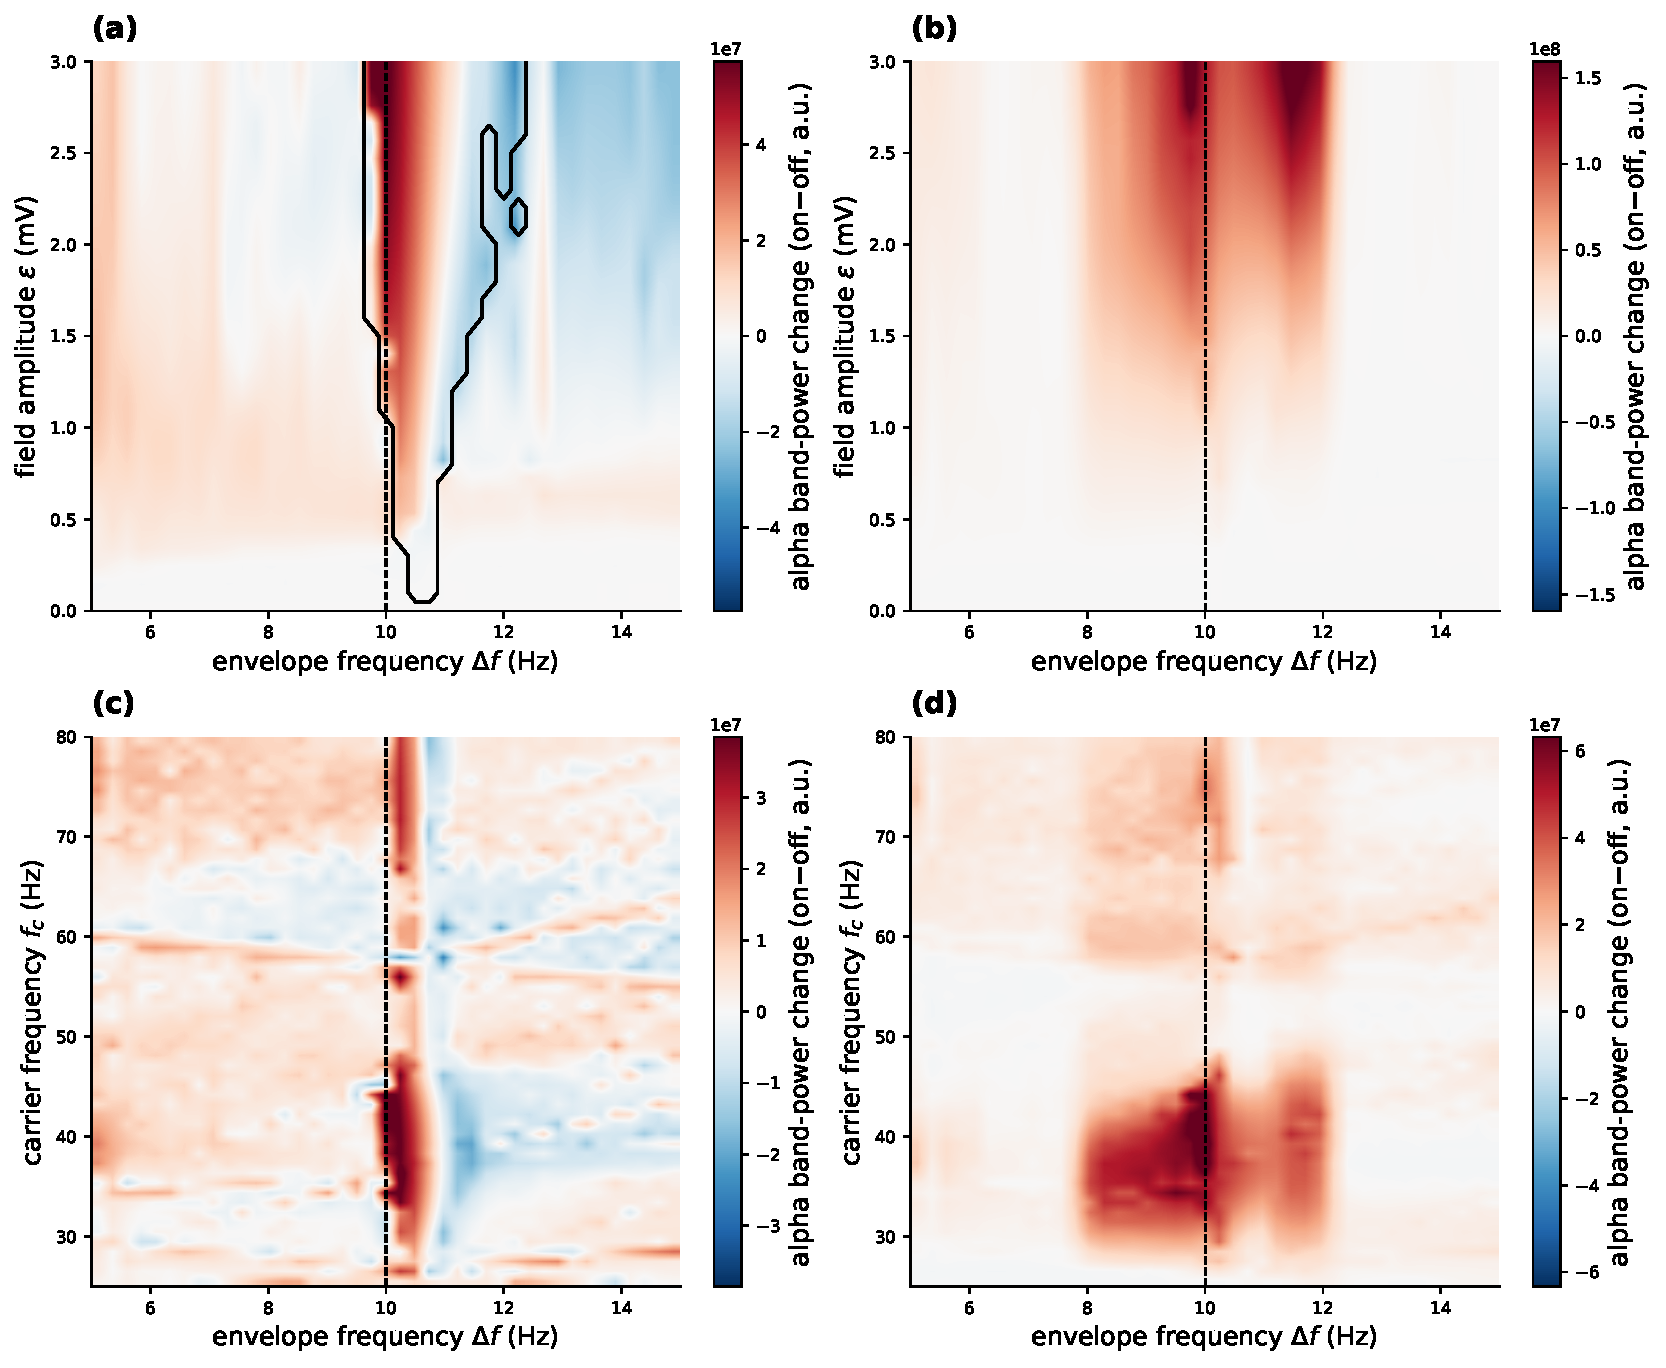
\includegraphics[width=0.86\textwidth]{fig_lanmm_field_p2_twotone.pdf}
\caption{\textbf{LaNMM Arnold tongues: two-tone TI field on the superficial $P_2$ (gamma)
loop.} The field enters the $P_2$ sigmoid argument as a membrane polarization $\varepsilon$
(mV) with all external drives flat. Color shows the signed change of alpha-band
($8$--$12$~Hz) power from the unstimulated $\varepsilon=0$ baseline, on a zero-centered
scale (arbitrary units). \emph{(a,b)} $P_1$ and $P_2$ enhancement vs.\
$\varepsilon$ and $\Delta f$ (carrier $40$~Hz), peaking at the $P_1$ alpha ($10.0$~Hz,
dashed). The black contour in \emph{(a)} is the frequency-dominance set
$|f_{\rm out}-\Delta f|<0.3$~Hz (Appendix~\ref{sec:vocab}), drawn because band power
alone cannot separate a driven from an autonomous rhythm; it is a dominance screen, not a
phase-capture test. The $\varepsilon=0$ row is excluded, since with no drive the
autonomous $10.67$~Hz alpha already lies within the tolerance of two grid points (a
resolution floor of $0.5$~Hz); the set widens to $2.75$~Hz at $3$~mV. \emph{(c,d)} Enhancement vs.\ carrier and $\Delta f$ at
$\varepsilon=1.5$~mV: $P_1$ demodulation needs \emph{both} a carrier near the $P_2$ gamma
($\approx 44$~Hz) and $\Delta f$ near the $P_1$ alpha---a double resonance.}
\label{fig:lanmm_p2}
\end{figure}

Concretely the LaNMM predicts that TI efficacy should (i) peak when $\Delta f$
matches a region's intrinsic alpha; (ii) widen and strengthen with modulation
amplitude (the tongue); and (iii) for fields delivered via superficial fast
circuits, be largest when the carrier is matched to a gamma network
\DIFdelbegin \DIFdel{resonance---e.g.\ }\DIFdelend \DIFaddbegin \DIFadd{resonance, for example }\DIFaddend two nearby gamma carriers summing to a $\sim$40~Hz-centered AM
\DIFdelbegin \DIFdel{field---while }\DIFdelend \DIFaddbegin \DIFadd{field, while }\DIFaddend remaining present, weaker, for off-resonance carriers. The third is
untested: existing TI studies of deep targets sweep the \emph{beat} frequency rather than
the carrier against a network resonance \cite{esmaeilpour2021,violante2023}, so they
neither support nor contradict it.

\section{Vocabulary and metrics}\label{sec:vocab}
The three terms (forced response, entrainment, gating) are defined in Methods; this
appendix gives the metrics behind them.
\emph{(i) Forced response.} Below the Hopf the column does not oscillate on its own; the
field elicits a driven response whose susceptibility we quantify by the lock-in amplitude
of the read-out at the beat $\Delta f$ (Eq.~\eqref{eq:lockin}), and there is no autonomous
rhythm to entrain (J-curve, timing, tACS).
\emph{(ii) Frequency entrainment.} Above the Hopf the column free-runs at $f_0$; genuine
entrainment means its dominant frequency is \emph{pulled} to $\Delta f$. We screen for it with
the dominant output frequency $f_{\rm out}$ (largest non-DC FFT peak) and the criterion
$|f_{\rm out}-\Delta f|<0.3$~Hz, mapping the tongue and locking range
(Fig.~\ref{fig:entrain}); $f_{\rm out}$ is used rather than a phase-locking value
\cite{lachaux1999} because, when an autonomous rhythm and a driven component coexist,
instantaneous-phase estimates conflate them. The dominance criterion is a screen, not a
capture test: the largest peak can move to the drive frequency because a driven component
outgrows a persisting autonomous one. A capture test would follow the unwrapped phase
difference and require the absence of secular drift; the maps therefore label the set the
frequency-dominance set.
\emph{(iii) Envelope locking / gating.} A periodic drive can instead modulate the
\emph{amplitude} of a persisting rhythm at the beat without capturing its
\DIFdelbegin \DIFdel{frequency---phase--amplitude coupling}\DIFdelend \DIFaddbegin \DIFadd{frequency (phase--amplitude coupling) }\DIFaddend \cite{canolty2010,tort2010}. We quantify this by
the $\Delta f$-locked component of the population rate (lock-in of $r_E$ at $\Delta f$,
equivalently the rate \emph{folded} on the $\Delta f$ beat \DIFdelbegin \DIFdel{phase---averaged }\DIFdelend \DIFaddbegin \DIFadd{phase, averaged }\DIFaddend over many beat
cycles as a function of phase within a single cycle, so that everything not locked to
$\Delta f$ averages away), which isolates the driven envelope from the intrinsic rhythm (the above-Hopf QIF panel,
with its $\sim$11~Hz detuning, is a case of gating, not entrainment).

The Arnold-tongue protocol for Fig.~\ref{fig:entrain} places the column on the limit-cycle side (input $p$ between the SNIC and the Hopf, free-running at $f_0(p)$) and drives it with $s(t)=\varepsilon\cos\Omega t$; the implementation, including the grid widths and the clipping check, is in the released code. One subtlety: as onset is approached the cycle amplitude vanishes and the tongue merges into the forced-resonance bandwidth, so the supercritical locking range and the subcritical $1/\gamma$ susceptibility coincide there by construction---which is why responsiveness peaks at criticality on both sides.

\section{Supplementary figures}

\begin{figure}[t!]
\centering
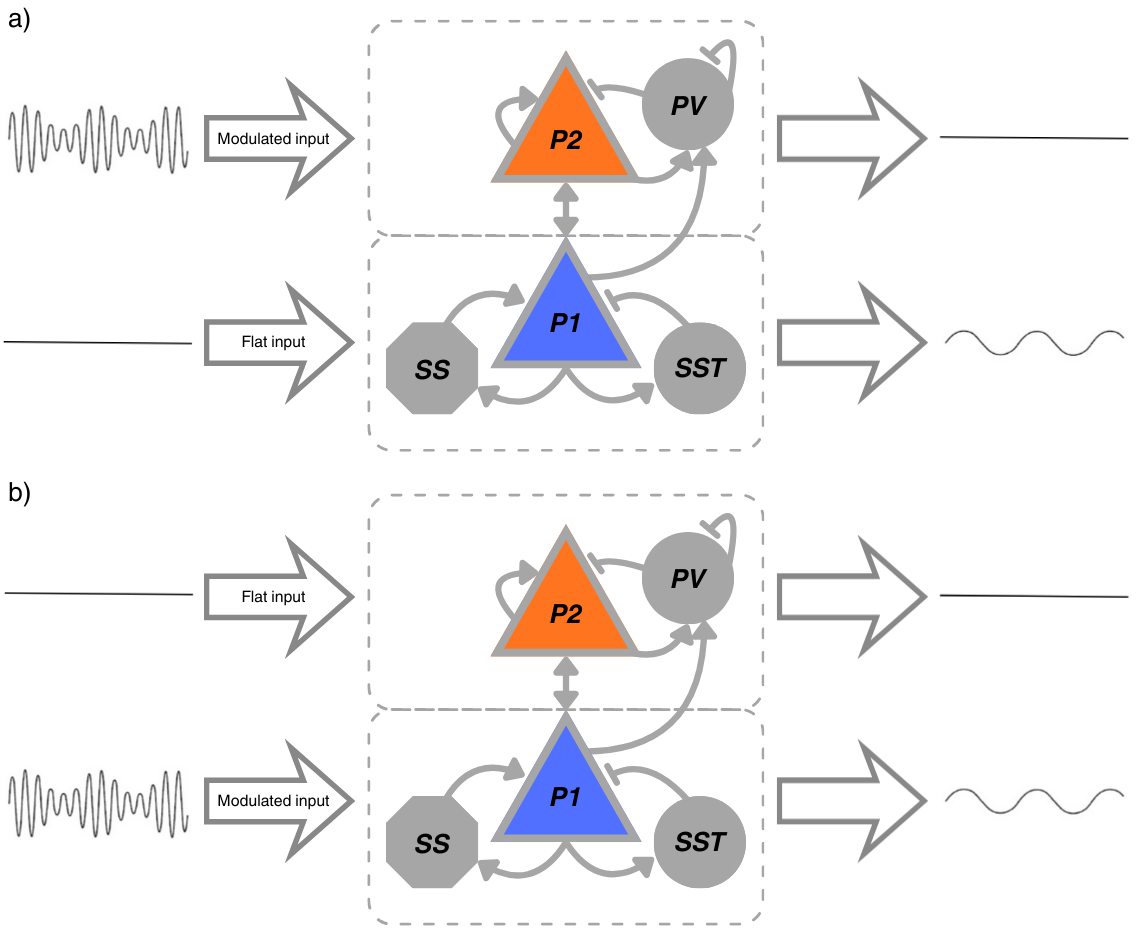
\includegraphics[width=0.85\textwidth]{fig_lanmm_setup.png}
\caption{\textbf{Stimulation setup in a LaNMM column.} The column couples a
superficial PING subcircuit (pyramidal $P_2$ + PV; gamma) and a deep JR
subcircuit (pyramidal $P_1$ + SS + SST; alpha). \emph{(a)} the TI field drives
$P_2$ while $P_1$ receives a flat drive; \emph{(b)} the TI field drives $P_1$
while $P_2$ is flat. Through the sigmoid nonlinearities and $P_1$--$P_2$ coupling,
the generated beat-frequency component is transferred to the deep loop: $P_2$ carries the
modulated fast carrier, while $P_1$ exposes the recovered low-frequency component (right
traces).}
\label{fig:lanmm_setup}
\end{figure}



\begin{figure}[t!]
\centering
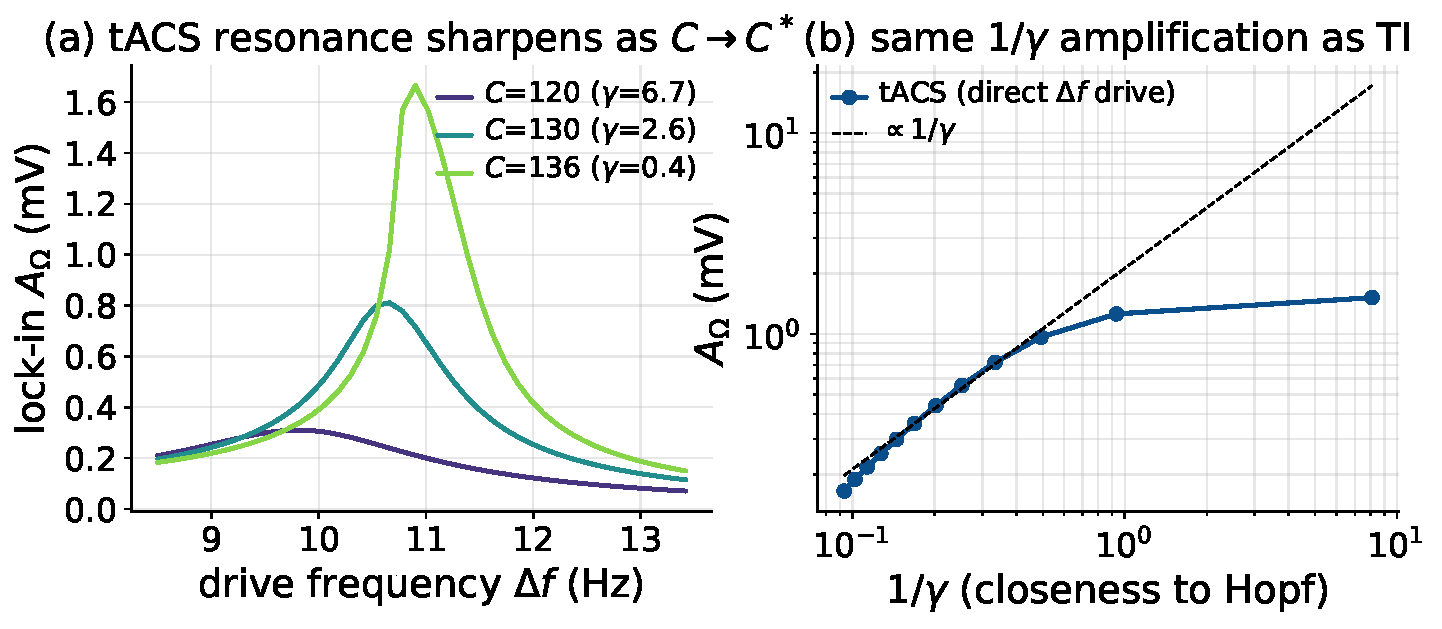
\includegraphics[width=0.92\textwidth]{fig_tacs_jcurve.pdf}
\caption{\textbf{tACS shares the network amplifier (Jansen--Rit).} A direct
low-frequency (tACS) drive at $\Delta f$ enters the column without a carrier, so it
needs no demodulation, but feeds the same near-Hopf resonator. With the operating point
pinned, sweeping the coupling $C\,(=J)$ toward the alpha Hopf: \emph{(a)} the lock-in
resonance at $\Delta f$ sharpens and grows as $C\!\to\!C^*$; \emph{(b)} the response
grows as $1/\gamma$ (dashed) and saturates near criticality---the same network
amplification as the demodulated TI drive (Fig.~\ref{fig:jcurve}), but linear in the
field rather than square-law. Throughout, the column is a stable focus ($\gamma>0$).}
\label{fig:tacs}
\end{figure}

\begin{figure}[t!]
\centering
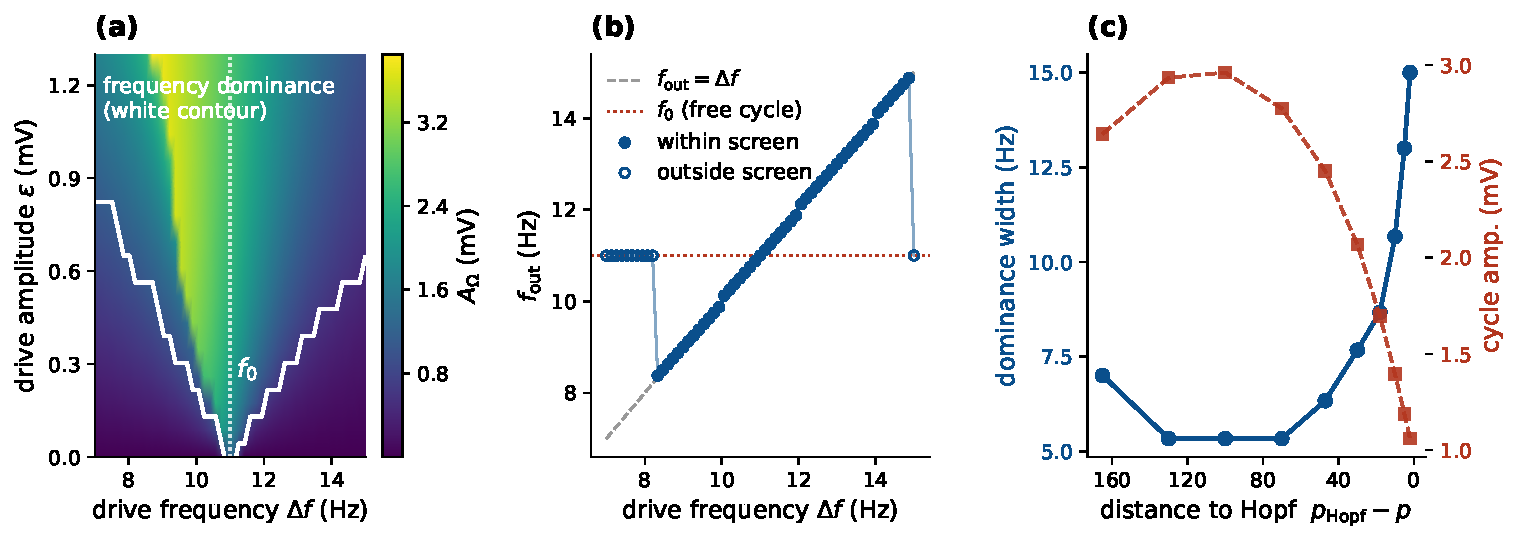
\includegraphics[width=\textwidth]{fig_entrainment.pdf}
\caption{\textbf{Above the Hopf: entrainment, not $1/\gamma$ amplification (Jansen--Rit).}
The column is set in its autonomous alpha limit cycle ($p=250$, $f_0\!\approx\!11$~Hz) and
driven by a direct in-band sinusoid. \emph{(a)} The $1{:}1$ Arnold \DIFdelbeginFL \DIFdelFL{tongue---where }\DIFdelendFL \DIFaddbeginFL \DIFaddFL{tongue, where }\DIFaddendFL the
dominant output frequency locks to $\Delta f$\DIFdelbeginFL \DIFdelFL{---is }\DIFdelendFL \DIFaddbeginFL \DIFaddFL{, is }\DIFaddendFL a wedge anchored at $f_0$ that widens
with drive. \emph{(b)} Inside the tongue the output follows $\Delta f$; outside, it falls
back to $f_0$. \emph{(c)} Toward the Hopf at fixed drive the locking range grows as the
autonomous cycle amplitude vanishes (blue, left axis; red dashed, right axis). Above the
Hopf amplification reads as tongue width rather than as the diverging $1/\gamma$ gain of
the stable-focus side (Fig.~\ref{fig:jcurve}): the column is most responsive near
criticality on both sides.}
\label{fig:entrain}
\end{figure}

\begin{figure}[t!]
\centering
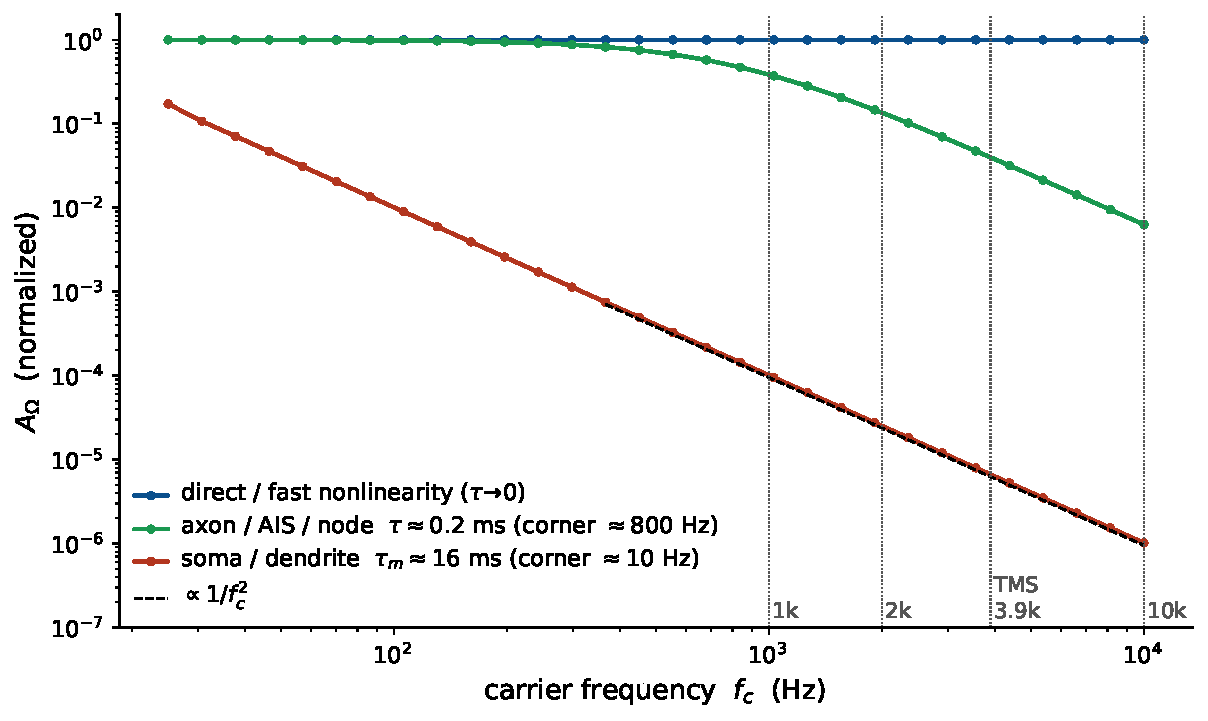
\includegraphics[width=0.74\textwidth]{fig_khz.pdf}
\caption{\DIFdelbeginFL \DIFdelFL{\textbf{Somatic demodulation dies at kHz, but a fast element survives (Jansen--Rit, open-loop detector).} }\DIFdelendFL \DIFaddbeginFL \DIFaddFL{\textbf{Carrier attenuation depends on the assumed access time (Jansen--Rit, open loop).} }\DIFaddendFL Open-loop
demodulated response (normalized to the $\tau\!\to\!0$ value) vs.\ carrier
frequency up to $10$~kHz. With direct coupling ($\tau\!\to\!0$) the response is
flat---carrier-independent. A slow somatic membrane ($\tau_m\!\approx\!16$~ms)
rolls off as $1/f_c^2$ (dashed guide)\DIFdelbeginFL \DIFdelFL{, killing kHz demodulation}\DIFdelendFL ; \DIFdelbeginFL \DIFdelFL{a }\DIFdelendFL \DIFaddbeginFL \DIFaddFL{the assumed }\DIFaddendFL fast \DIFdelbeginFL \DIFdelFL{element
}\DIFdelendFL \DIFaddbeginFL \DIFaddFL{response
}\DIFaddendFL (\DIFdelbeginFL \DIFdelFL{axon/AIS/node, $\tau\!\approx\!0.2$}\DIFdelendFL \DIFaddbeginFL \DIFaddFL{$\tau=0.2$}\DIFaddendFL ~ms) retains \DIFdelbeginFL \DIFdelFL{an appreciable response into }\DIFdelendFL \DIFaddbeginFL \DIFaddFL{about $0.14$ of }\DIFaddendFL the \DIFdelbeginFL \DIFdelFL{kHz band ($\sim$0.14 }\DIFdelendFL \DIFaddbeginFL \DIFaddFL{direct response }\DIFaddendFL at \DIFdelbeginFL \DIFdelFL{2}\DIFdelendFL \DIFaddbeginFL \DIFaddFL{$2$}\DIFaddendFL ~kHz \DIFdelbeginFL \DIFdelFL{, $\sim$0.04 }\DIFdelendFL \DIFaddbeginFL \DIFaddFL{and $0.04$
}\DIFaddendFL at \DIFdelbeginFL \DIFdelFL{the TMS peak }\DIFdelendFL $3.9$~kHz\DIFdelbeginFL \DIFdelFL{)}\DIFdelendFL . \DIFdelbeginFL \DIFdelFL{The same
membrane filter attenuates TMS at the soma}\DIFdelendFL \DIFaddbeginFL \DIFaddFL{These are sensitivity cases}\DIFaddendFL , \DIFdelbeginFL \DIFdelFL{which is why neither TMS nor TI should
be thought }\DIFdelendFL \DIFaddbeginFL \DIFaddFL{not measurements }\DIFaddendFL of \DIFdelbeginFL \DIFdelFL{as driving the soma at kHz}\DIFdelendFL \DIFaddbeginFL \DIFaddFL{anatomical
compartments}\DIFaddendFL .}
\label{fig:khz}
\end{figure}
\begin{figure}[t!]
\centering
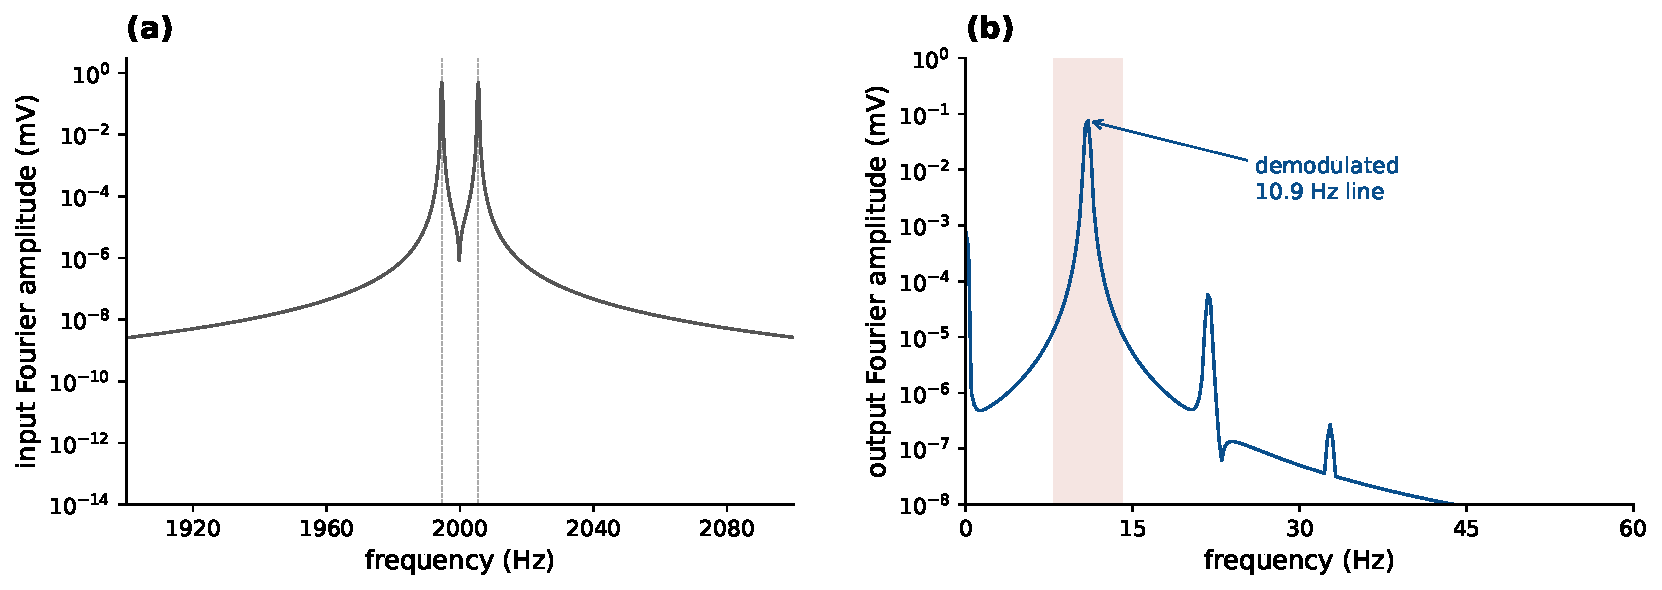
\includegraphics[width=0.95\textwidth]{fig_khz_twotone.pdf}
\caption{\DIFdelbeginFL \DIFdelFL{\textbf{Genuine two-tone TI at a real kHz carrier (Jansen--Rit, fast-element
route).} }\DIFdelendFL \DIFaddbeginFL \DIFaddFL{\textbf{Two-tone TI at a kHz carrier (Jansen--Rit, assumed fast access).}
}\DIFaddendFL Two equal tones at $f_1=1994.54$ and $f_2=2005.46$~Hz, beating at \DIFdelbeginFL \DIFdelFL{$10.91$}\DIFdelendFL \DIFaddbeginFL \DIFaddFL{approximately
$10.9$}\DIFaddendFL ~Hz, pass through the \DIFdelbeginFL \DIFdelFL{fast-element }\DIFdelendFL \DIFaddbeginFL \DIFaddFL{assumed }\DIFaddendFL low-pass ($\tau=0.2$~ms) into the recurrent column.
\emph{(a)} The input amplitude spectrum has lines only at $f_1$ and $f_2$; in the
$8$--$14$~Hz band it is $2.2\times10^{-13}$, zero to numerical precision.
\emph{(b)} The output carries a demodulated line at the beat, $10.9$~Hz.}
\label{fig:khz_twotone}
\end{figure}
\begin{figure}[t!]
\centering
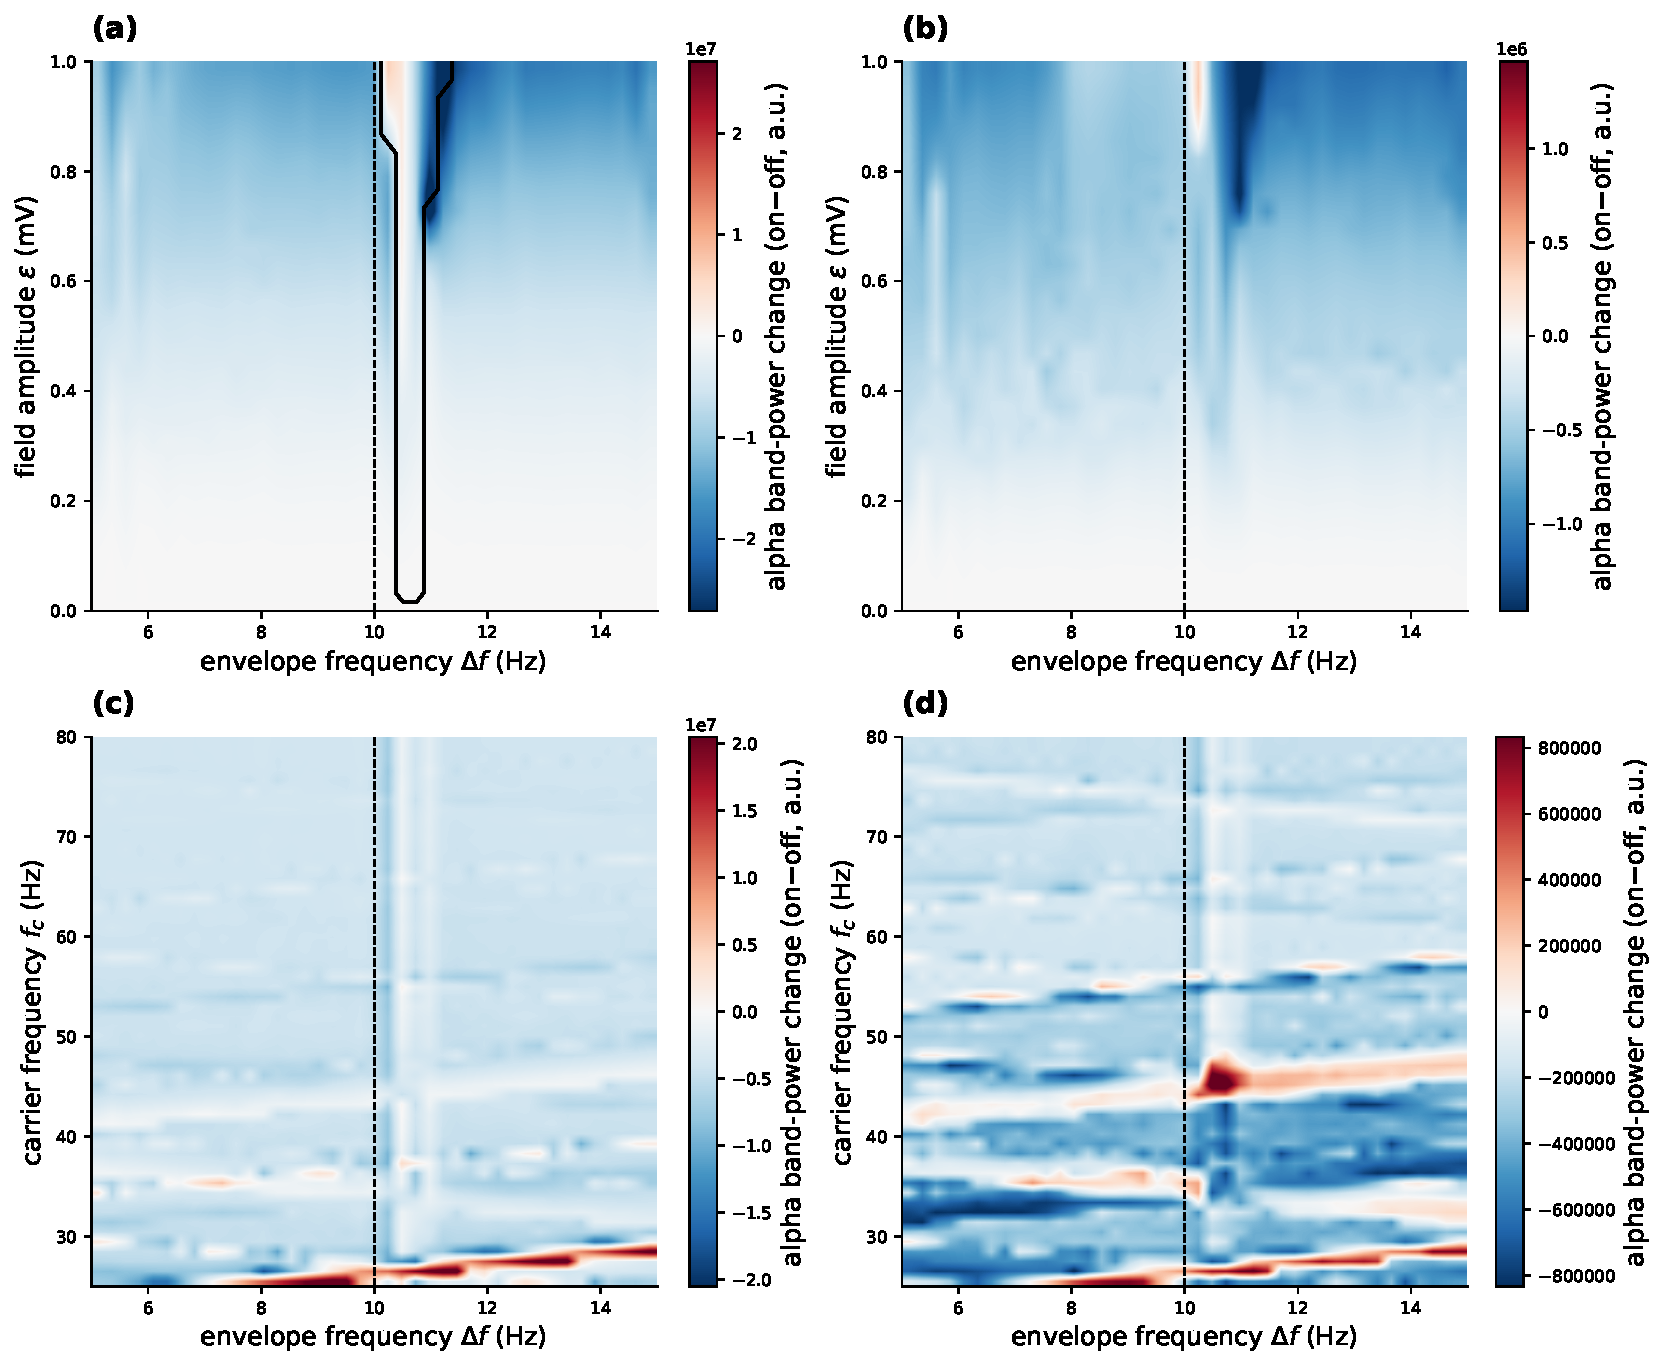
\includegraphics[width=0.86\textwidth]{fig_lanmm_field_p1_twotone.pdf}
\caption{\textbf{LaNMM Arnold tongues: two-tone TI field delivered directly to the deep
$P_1$ (alpha) loop.} As Fig.~\ref{fig:lanmm_p2} but with the field on $P_1$. The deep loop
is captured by a much weaker field than the superficial one, so the amplitude range is
$\varepsilon\le1$~mV here against $3$~mV there; above $\approx 2$~mV the drive captures
\DIFdelbeginFL \DIFdelFL{essentially }\DIFdelendFL the whole $\Delta f$ sweep and leaves the perturbative regime the theory
describes. Color: signed change of alpha-band power from the $\varepsilon=0$ baseline,
zero-centered; most of the grid is suppression. \emph{(a,b)} $P_1$ and $P_2$ enhancement vs.\ $\varepsilon$ and $\Delta f$; the
black contour in \emph{(a)} outlines the frequency-dominance set
$|f_{\rm out}-\Delta f|<0.3$~Hz (Appendix~\ref{sec:vocab}), computed from the dominant
output frequency because band power alone cannot separate a driven from an autonomous
rhythm; the $\varepsilon=0$ row is excluded (resolution floor $0.5$~Hz). The set widens to
$1.25$~Hz at $\varepsilon=1$~mV.
\emph{(c,d)} Enhancement vs.\ carrier frequency and $\Delta f$ at $\varepsilon=0.5$~mV.
$P_1$ responds across a \emph{broad} carrier band---a vertical ridge at
$\Delta f\!\approx\!10$~Hz, the direct-coupling limit of Eq.~\eqref{eq:demod}. Read with
the lock-in at $\Delta f$ the response is retained at every carrier from $25$ to $80$~Hz
(median $25\%$ of peak), in contrast to the $\sim$7\% collapse off resonance under
superficial drive.}
\label{fig:lanmm_p1}
\end{figure}
\begin{figure}[t!]
\centering
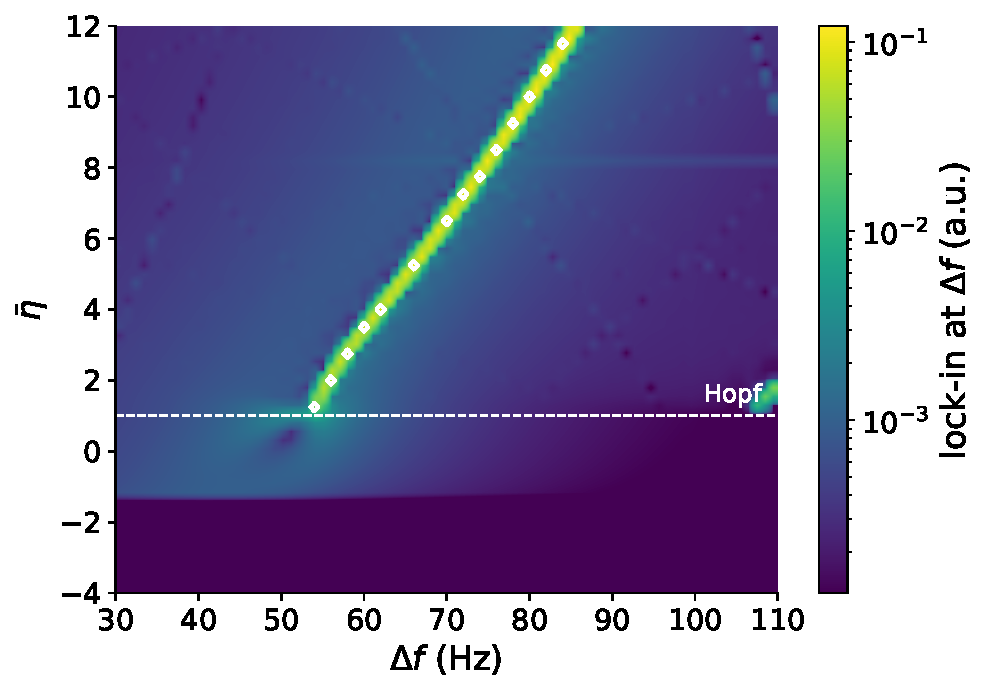
\includegraphics[width=0.72\textwidth]{fig_nmm2_map.pdf}
\caption{\textbf{NMM2 PING resonance map (exact mean field).} Demodulated response over
the ($\Delta f$, background drive $\bar\eta$) plane, log color scale. The ridge follows the
gamma natural frequency, \DIFdelbeginFL \DIFdelFL{and its diagonal slope---}\DIFdelendFL \DIFaddbeginFL \DIFaddFL{with }\DIFaddendFL $f_0$ rising with $\bar\eta$ \DIFdelbeginFL \DIFdelFL{---reflects
the state-dependent transfer of NMM2, absent in the static-sigmoid models}\DIFdelendFL \DIFaddbeginFL \DIFaddFL{for these parameters}\DIFaddendFL . White markers
outline the $1{:}1$ captured set (Appendix~\ref{sec:vocab}), drawn only above the Hopf
(dashed line) where there is an autonomous rhythm to capture; below it the same color field
is a forced response. Lock-in amplitude cannot separate the two, since both place power at
$\Delta f$.}
\label{fig:nmm2_map}
\end{figure}


\begin{figure}[t!]
\centering
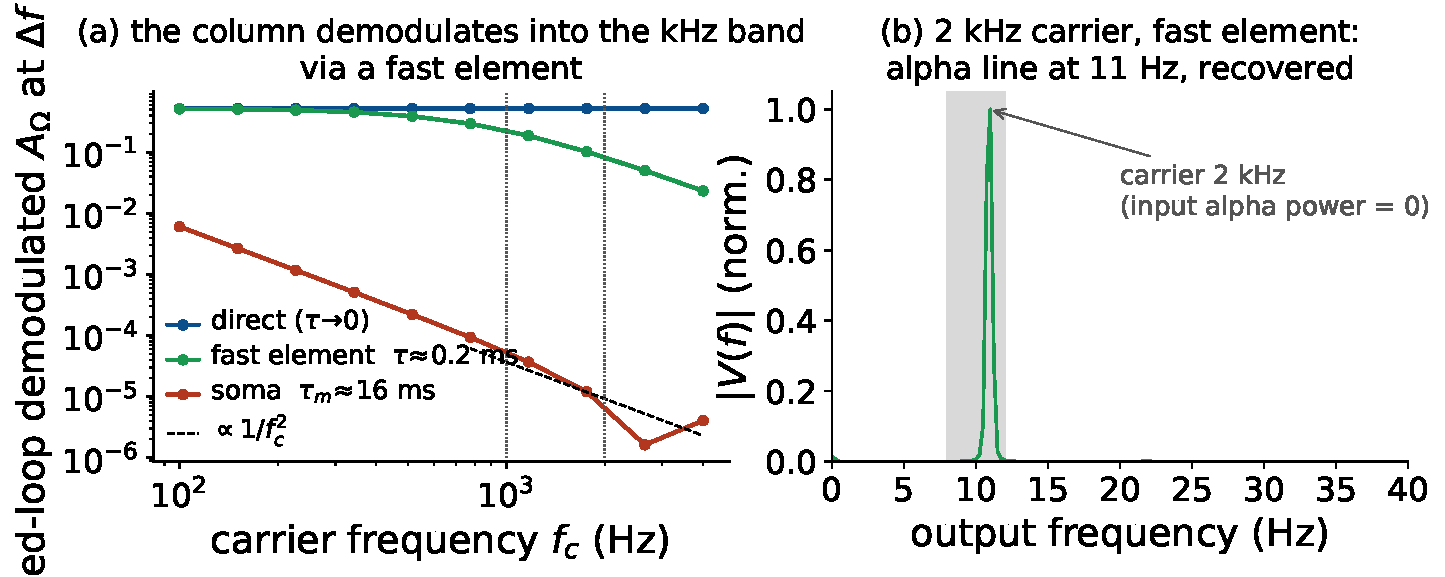
\includegraphics[width=\textwidth]{fig_khz_direct.pdf}
\caption{\textbf{Demodulation at a genuine kHz carrier (Jansen--Rit, closed loop).}
The applied field passes through an explicit membrane filter before the sigmoid.
\emph{(a)} Closed-loop demodulated $A_\Omega$ at $\Delta f=f_0$ vs.\ carrier $f_c$ for
three \DIFdelbeginFL \DIFdelFL{coupling routes}\DIFdelendFL \DIFaddbeginFL \DIFaddFL{access models}\DIFaddendFL : direct ($\tau\!\to\!0$, carrier-independent), fast
\DIFdelbeginFL \DIFdelFL{element
}\DIFdelendFL (\DIFdelbeginFL \DIFdelFL{axon/AIS/node, $\tau\!\approx\!0.2$}\DIFdelendFL \DIFaddbeginFL \DIFaddFL{$\tau=0.2$}\DIFaddendFL ~ms\DIFdelbeginFL \DIFdelFL{; survives into the kHz band}\DIFdelendFL ), and \DIFdelbeginFL \DIFdelFL{soma
}\DIFdelendFL \DIFaddbeginFL \DIFaddFL{somatic }\DIFaddendFL (\DIFdelbeginFL \DIFdelFL{$\tau_m\!\approx\!16$}\DIFdelendFL \DIFaddbeginFL \DIFaddFL{$\tau_m=16$}\DIFaddendFL ~ms; \DIFdelbeginFL \DIFdelFL{collapses as }\DIFdelendFL $1/f_c^2$ \DIFaddbeginFL \DIFaddFL{roll-off}\DIFaddendFL )\DIFaddbeginFL \DIFaddFL{.
The fast time is assumed rather than assigned to a measured compartment}\DIFaddendFL .
\emph{(b)} Output spectrum for a
$2$~kHz carrier delivered through the fast element: a clean alpha line at $f_0$,
synthesized by the column although the input carries no alpha power.}
\label{fig:khz_direct}
\end{figure}

\begin{figure}[t!]
\centering
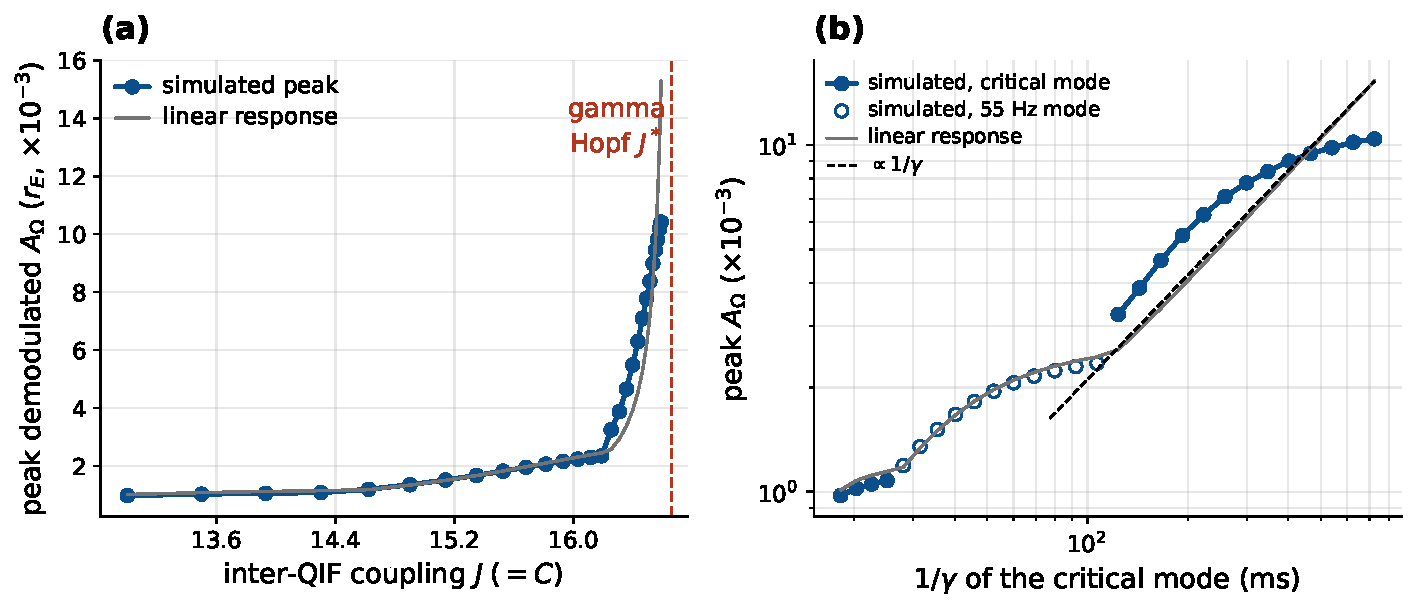
\includegraphics[width=0.92\textwidth]{fig_nmm2_jcurve.pdf}
\caption{\textbf{Coupling controls the amplification in the exact mean field (NMM2
PING, gamma).} $J\,(=C)$ is the literal inter-QIF synaptic weight; at this carrier the generated
source is operating-point independent (\S\ref{sec:dynamic}), so no pinning is needed.
\emph{(a)} The peak demodulated response of $r_E$ grows as $J\!\to\!J^*$ (gamma
Hopf, $\bar\eta=0$; stable focus, $\gamma>0$). \emph{(b)} The gain grows as $1/\gamma$ (dashed), saturating near
criticality---the JR law, now with coupling and rectifier both derived.}
\label{fig:nmm2_jcurve}
\end{figure}

\begin{figure}[t!]
\centering
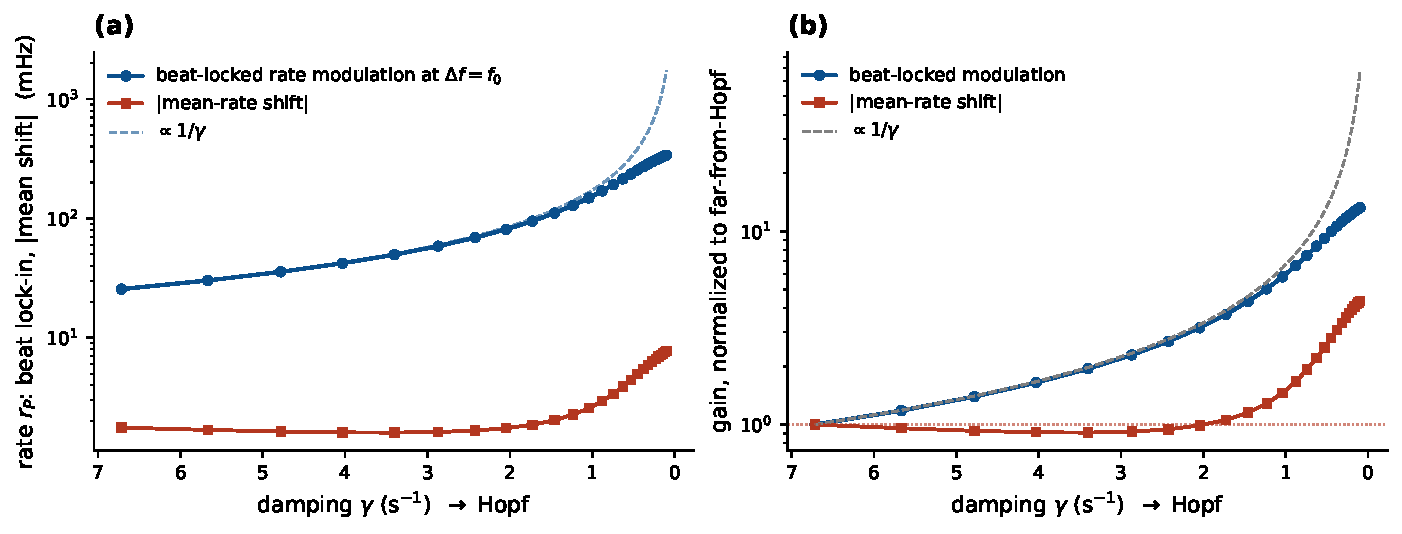
\includegraphics[width=\textwidth]{fig_timing_not_rate.pdf}
\caption{\textbf{Envelope-locked modulation against mean-rate shift (Jansen--Rit,
detection pinned).} As the column is driven toward the Hopf (from the stable side,
$\gamma>0$) through the coupling at fixed $\Sig''(v^*)$, both quantities are read from the
pyramidal rate $r_P=\Sig(v+s)$, in mHz. \emph{(a)} The beat-locked modulation at
$\Delta f=f_0$ (blue) is resonantly amplified and tracks $1/\gamma$ (dashed) before
saturating; the magnitude of the mean-rate shift (red) stays at a few mHz and rises near
the Hopf. \emph{(b)} Both normalized to their far-from-Hopf values (log scale): the
modulation gain follows $1/\gamma$; the mean-shift gain rises later and less. Modulation
exceeds mean shift by $19\times$ far from the Hopf and $45$--$66\times$ near it.}
\label{fig:timing}
\end{figure}

\begin{figure}[t!]
\centering
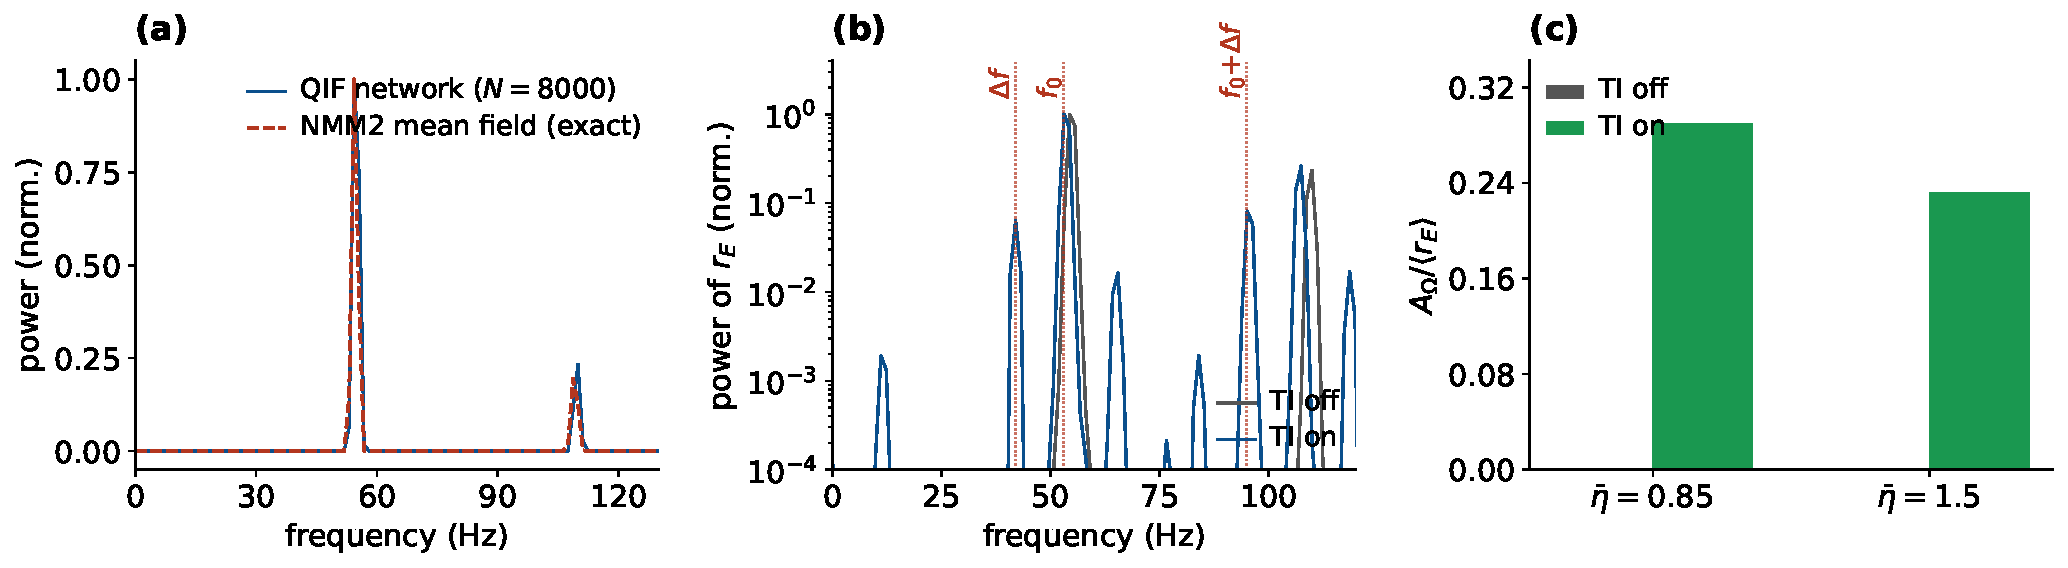
\includegraphics[width=\textwidth]{fig_qif_timing_twotone.pdf}
\caption{\textbf{Timing, not rate, in the QIF network.} \emph{(a)} Field-free power
spectrum of $r_E(t)$, normalized: the spiking network ($N=8000$) matches the exact NMM2
mean field in gamma frequency ($\sim$53~Hz); a normalized spectrum does not test the mean
rate. \emph{(b)} Intermodulation above the
Hopf (TI off vs.\ on, log power): the nonlinearity mixes the imposed $\Delta f=42$~Hz beat
with the intrinsic $53$~Hz gamma, raising the direct $\Delta f$ line and the sum sideband
near $95$~Hz, both absent with TI off. This is the sideband signature of gating rather
than entrainment. \emph{(c)} The $\Delta f$ modulation depth
$A_\Omega/\langle r_E\rangle$, off vs.\ on: below $0.003$ rising to $0.29$ (forced) and
$0.23$ (oscillatory), while the mean rate rises by $8$--$10\%$. Modulation depth is
reported rather than the off$\to$on lock-in ratio, whose denominator is the field-free
floor.}
\label{fig:qif_timing}
\end{figure}


% The supplement cites a handful of works (locking metrics, normal-form theory)
% and is read as a standalone file, so it carries its own reference list.
\ifsupp
\clearpage
\bibliographystyle{unsrt}
\bibliography{references}
\fi
\fi
\end{document}
